% !TeX spellcheck = en_US
\documentclass[11pt,a4paper,twocolumn]{book}
\usepackage[latin1]{inputenc}
\usepackage{amsmath}
\usepackage{amsfonts}
\usepackage{amssymb}
\usepackage{graphicx}
\usepackage[table]{xcolor}
\usepackage{wrapfig}
\usepackage{multicol}
\usepackage{multirow}
\usepackage{paralist}
\usepackage{longtable}
\usepackage{tabu}
\usepackage{soul}
\usepackage{titling}
\usepackage{pdfpages}
\usepackage[hidelinks]{hyperref}


\hypersetup{
	colorlinks,
	citecolor=black,
	filecolor=black,
	linkcolor=black,
	urlcolor=black,
	bookmarks=true
}

\title{Mutant Manual}


\begin{document}
	
	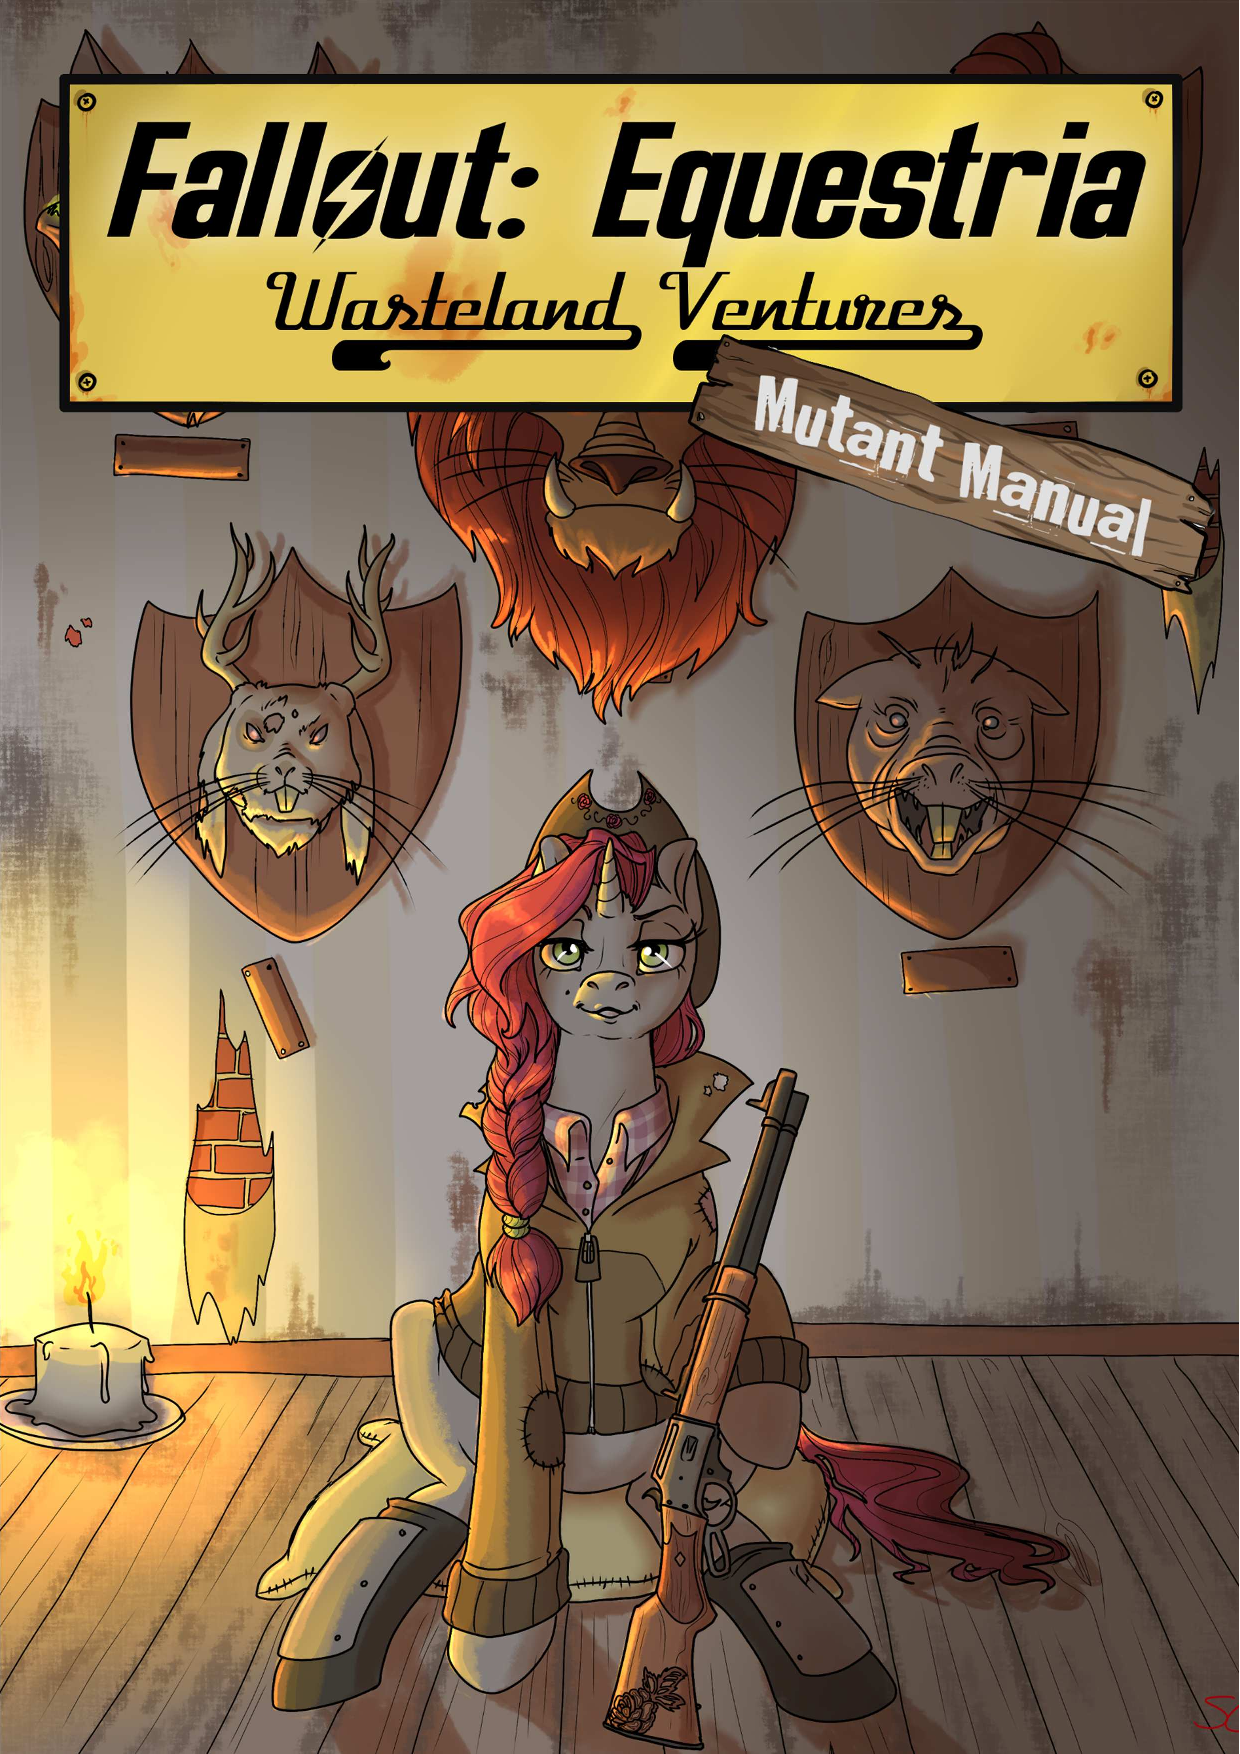
\includepdf[pages={1}]{WORD/COVER-MUMA.pdf}	
	\onecolumn	
	\setcounter{page}{1}
	
	\begin{center}
		Compiled by Waak, Kireanikin, LaPa, Miksu \& SourCherry
		
		\bigskip
		\textbf{Additional Monsters \& Help:} El Dee, LZ, Yondalor
		
		\bigskip
		\textbf{Cover \& Graphics:} SourCherry
		
		\bigskip
		\textbf{Layout:} Waak
		
	\end{center}
	
	\begin{figure*}[bp]
		\centering
		
\includegraphics[width=3cm]{ART/ISA_Logo}
		\label{fig:isalogo}
	\end{figure*}
	
	\twocolumn
	
	\tableofcontents	
	
	
	\chapter{Introduction}
	\begin{quote}
		\emph{``Well, sonny, headin' out to the big bad Wasteland is goin' to be a harrowing experience for ya unless ya go prepared. Ah've spent a good chunk of mah life gatherin' notes and stuff to prepare a wet-behind-the-ears foal for this moment... Hope it helps ya.''}
	\end{quote}
	
	The world of post-apocalypse Equestria is filled with a variety of creatures with most out to get your head. This book seeks to give examples of creatures that populate the many different places in the Wasteland, from the darkest ruins to open plains and beyond.
	
	These creatures, both sentient and not, serve as the many antagonists and obstacles to the players' characters, and to give them conflict to solve, either by speaking the forces opposing them down or by giving them a solid whacking. More often than not, it's the solid whacking.
	
	Though this book offers statistics to the monsters both mutated and not, they should be seen more as guidelines than hard facts, and can be tinkered with to suit the purpose of the story and the party level.
	
	\clearpage
	
	\chapter{Rules}

	\section*{Types of Mutants}
%	\addcontentsline{toc}{section}{Types of Mutants}
	Mutants have many different types, which can mean they resist or are outright immune to some of the game's concepts. This chapter also focuses on explaining what the common guidelines are for the various creatures that belong into a particular grouping.
	
	Creatures, both sentient and ``feral'' have an assortment of skills they generally utilize. Most are due to training and innate abilities and features. These are for quick access and reference. In a situation, where player characters use skills against unspecified values, such as Barter to strike a deal with an Equitron, creatures use either an untrained value of 15 or 20, or freely given values to create individuality to said creatures.
	
	\begin{verse}
		\emph{\textbf{Note:} Certain creatures, such as most insects and robots have additional body parts (antennae and combat inhibitors exclusively) that are considered limbs and which can be crippled. Hitting these parts will cause the creature to be unable to discern enemies and friends and attack the closest creature next to it.}
	\end{verse}
	
	\begin{description}		
		\item[Abomination:]  What commonly differentiates Abominations from other Mutants is often the lack of proper adaptation and evolution to the Wasteland. Resemblance of Abominations usually stands out like something forcibly changed them to their state, without any consideration whether change was beneficial. Abominations have, however, developed or gained many magical and necrotic abilities beyond most magicians. They can often also be traced back to species that was or is sentient.
		\item[Animal:] Animals are perhaps the most diverse creatures of the bunch, and unlike other creatures, do not have any special rules for them.
		\item[Insect:] Insects have their own caste from animals as they have chitinous exoskeleton and often a pair of antennae as well as three pair of legs. This means insects usually have more legs to cripple, functioning relatively well even if two of their legs are out, but their antennae are also a part for crippling effect; this effect causes the insect to gain Mind-Controlled and Enraged status effects.
		\item[Machine:] Machines are creations of science, hulking metallic creations varying from simply automated turrets to robots of very equine characteristics. Common to all robots is their fearlessness, making Intimidation pointless against them, inability to bleed like living creatures, and their inability to feel pain, keeping them functioning even with critical damage. Machines do bear weakness to EMP based weapons and can be shutdown.
		\item[Mutant:] Mutant means that the creature was mutated from some Pre-War era creature either by balefire or Taint. These are the most common creatures in the manual. Mutants have a higher tolerance to radiation but are often not immune to it.
		\item[Non-Mutant:] Non-Mutated creatures are the ones that due to immunity to radiation and taint have remained the same even after the apocalypse. Their most notable trait is that radiation has no effect on them at all, rendering weapons that deal radiation damage moot against them.
		\item[Plant:] Plants are diverse, with various species being born of Radiation or Taint mutations, to completely remaining unscathed by them surviving from the times before war. Common trait to plants is their complete inability to move or simply move remarkably slow. However, plants cannot be Crippled.
		\item[Sentient:] Best way to describe Sentient beings is their ability to communicate with the common language, and think rationally; assuming they wish to do so. Sentient beings are most commonly other equines and griffons, thus their abilities and resiliencies are quite equal, each having fairly low Radiation tolerance and nearly zero chance to survive contamination by Taint. However, their nature can vary from highly sophisticated societies that can be interacted with ease to purely savage tribal groups that will see outsiders little more than prey.
		
	\end{description}	
	\vfill

	\section*{Looting Mutants}
%	\addcontentsline{toc}{section}{Looting Mutants}
	In the \emph{Mutant Manual}, each creature has a small collection of items listed for the players to loot for themselves. Aside from two exceptions looting doesn't require a check to perform. These exceptions are doubling the amount of particular item the character can get, and items that have a chance of being on the lootable character.
	
	Doubling the number of lootable items is usually done by rolling either \textbf{Survival}, \textbf{Mechanics} or \textbf{Science}. Items of this type have the required skill listed next to them. 
	
	Some items require a successful LCK roll for the item to be in the enemy's inventory. Such items are books, magic notes and magazines, which can be carried around by sentient creatures.
	
	In case of there being a large amount of downed enemies, the looting can be collective of all the creatures, to reduce the time the party spends pulling off armors and prying weapons from dead hooves.
	
	Due to these lists not being exhaustive and mentioning every part of a creature down to their pinky toes, PCs sometimes want to get parts that are not listed on the list. It is suggested that the GM looks at the possible skill requirements of a similar part and proceeds accordingly. These parts may require a Survival, Mechanics or Science roll for successful removal.
	
	After a PC has managed to find what they can from the downed enemy, the enemy is considered empty, even if another PC decided to go through them in more detail later.
	
	\onecolumn
	
	
	\chapter{Critters \& Mutants}
	
	\section*{Alicorns}
	\addcontentsline{toc}{section}{Alicorns}
	\begin{quote}
		\emph{``Rarely do you come across a creature more dangerous than an alicorn. Armed with Unicorn's powerful magic, Pegasi' flight and the tremendous strength of the Earth Pony, this smart abomination will kill you in a blink of an eye. And all other Alicorns will know it in a heartbeat.``}
			
	\emph{-	Star Paladin Glitter Dust}
	\end{quote}
	
	\subsection*{Blue Alicorn}
	\addcontentsline{toc}{subsection}{Blue Alicorn}
	\emph{\textbf{Type:} Abomination/Sentient}
	
	\noindent
	\emph{\textbf{EXP:} 250}
	
	{
		\rowcolors{1}{gray!30}{gray!10}
		\begin{tabu} to 150mm{| X[c,1] | X[c,1] | X[c,1] | X[c,1] | X[c,1] | X[c,1] | X[c,1] | X[c,1] |  X[c,3] | X[c,3]| X[c,3] | X[c,3] | X[c,3] |}
			\hline
			\multicolumn{13}{|c|}{\cellcolor{gray!50} Blue Alicorn Statistics} \\ \hline
			S & P & E & C & I & A & L & \cellcolor{gray!50} & HP & DT & AP & Size & Karma \\ 
			6 & 5 & 6 & 6 & 7 & 9 & 5 & \cellcolor{gray!50} & 16 & 25 & 14 & 1 & -25* \\ \hline
		\end{tabu}
	
		\emph{*Alicorn's Karma may fluctuate depending on setting}
	}
	
	\bigskip
	{
		\rowcolors{1}{gray!30}{gray!10}
		\begin{tabu} to 150mm{| X[c,1] | X[c,1] | X[c,1] | X[c,1] | X[c,1] |}
			\hline
			\multicolumn{5}{|c|}{\cellcolor{gray!50} Blue Alicorn Skills} \\ \hline
			 Melee & Unarmed & Sneak & Potency & Strain \\ 
			 75 & 50 & 60 & 14 & 40 \\ \hline
		\end{tabu}

	}
	
	\subsubsection*{Additional Combat Details:}
	\begin{verse}
		\textbf{Wasteland Weaponry:} Blue Alicorns equip themselves with weapons and armor, tending to favor light armor, and fight with various Melee and Unarmed.
		
		\textbf{Magical Talent:} The blue variant of the Alicorn has access to all the spells in the Conjuration and Illusion Magic Schools. Spells in these schools have -1 to their AP costs (to a minimum of 1).
		
		\textbf{Alicorn Magic:} Blue Alicorns have access to a powerful Invisibility-spell. Blue Alicorn's Invisibility gains +5 to Duration.
		
		\textbf{Super charged:} When exposed to high amounts of radiation, the Alicorns grow in size from 1 to 2. In addition, they can create a burst attack of irradiated glowing air to all adjacent to them. This attack deals 35+(3) damage and gives 2 Rads at 1x70\%, and costs 7 AP.
		
		Flying: Alicorns have working wings, thus they are capable of flight. Blue Alicorn's flight speed is 1 AP for 4 meters (2 Hexes). Alicorns have working wings, thus they are capable of flight. Blue Alicorn's flight speed is 1 AP for 4 meters (2 Hexes).
		
		\textbf{Poison Resistant:} Alicorns' Poison Resistance is 50.
		
		\textbf{Rad Immunity:} Alicorns are immune to Radiation.
		
	\end{verse}
		
	\subsubsection*{Creature drops:}
	\begin{compactitem}
		\item Abomination flesh piece (1d4, Survival doubles u.)
		\item Main Weapon (1)
		\item Additional Weapon (2)
		\item Armor (1)
		\item Spell Instructions, Conjuration/Illusion school (1, LCK-2 to obtain)
	\end{compactitem}

	\begin{figure}[h]
		\centering
		\includegraphics[width=0.7\linewidth]{"ART/Enemies/Alicorn Blue"}
	\end{figure}
	
	\vfill
	
	
	\subsection*{Green Alicorn}
	\addcontentsline{toc}{subsection}{Green Alicorn}
	\emph{\textbf{Type:} Abomination/Sentient}
	
	\emph{\textbf{EXP:} 200}
	
	{
		\rowcolors{1}{gray!30}{gray!10}
		\begin{tabu} to 150mm{| X[c,1] | X[c,1] | X[c,1] | X[c,1] | X[c,1] | X[c,1] | X[c,1] | X[c,1] |  X[c,3] | X[c,3]| X[c,3] | X[c,3] | X[c,3] |}
			\hline
			\multicolumn{13}{|c|}{\cellcolor{gray!50} Green Alicorn Statistics} \\ \hline
			S & P & E & C & I & A & L & \cellcolor{gray!50} & HP & DT & AP & Size & Karma \\ 
			8 & 7 & 6 & 4 & 5 & 7 & 5 & \cellcolor{gray!50} & 20 & 15 & 13 & 1 & -25* \\ \hline
		\end{tabu}
		
		\emph{*Alicorn's Karma may fluctuate depending on setting}
	}
	
	\bigskip
	{
		\rowcolors{1}{gray!30}{gray!10}
		\begin{tabu} to 150mm{| X[c,1] | X[c,1] | X[c,1] | X[c,1] | X[c,1] | X[c,1] |}
			\hline
			\multicolumn{6}{|c|}{\cellcolor{gray!50} Green Alicorn Skills} \\ \hline
			Firearms & Explosives & Mechanics & Sneak & Potency & Strain \\ 
			65 & 60 & 40 & 40 & 11 & 30 \\ \hline
		\end{tabu}
		
	}
		
	\subsubsection*{Additional Combat Details:}
	\begin{verse}
		\textbf{Wasteland Weaponry:} Green Alicorns equip themselves with weapons and armor, tending to favor heavy armor, and fight with various Firearms and Explosives with great efficiency.
		
		\textbf{Magical Talent:} This variant of the Alicorn has access to the Perception and Enchantment Magic schools. Spells in these schools have -1 to their AP costs (to a minimum of 1).
		
		\textbf{Alicorn Magic:} Green Alicorns have a powerful Shield Spell. Green Alicorn's Shield has 20 DT, and can stop explosives such as grenades and thrown weapons.
		
		\textbf{Super charged:} When exposed to high amounts of radiation, the Alicorns grow in size from 1 to 2. In addition, they can create a burst attack of irradiated glowing air to all adjacent to them. This attack deals 35+(3) damage and gives 2 Rads at 1x70\%, and costs 7 AP.
		
		\textbf{Flying:} Alicorns have working wings, thus they are capable of flight. Green Alicorn's flight speed is 1 AP for 6 meter (3 Hexes).
		
		\textbf{Poison Resistant:} Alicorns' Poison Resistance is 50.
		
		\textbf{Rad Immunity:} Alicorns are immune to Radiation.
	\end{verse}
	
	\subsubsection*{Creature drops:}
	\begin{compactitem}
		\item Abomination Flesh piece (1d4, Survival doubles u.)
		\item Main Weapon (1)
		\item Additional Weapon (1, Survival doubles u.)
		\item Armor (1)
		\item Spell Instruction, Perception/Enchantment School (1 u., LCK-2 to obtain)
	\end{compactitem}
	
	\vfill
	
	\subsection*{Purple Alicorn}
	\addcontentsline{toc}{subsection}{Purple Alicorn}
	\emph{\textbf{Type:} Abomination/Sentient}
	
	\emph{\textbf{EXP:} 300}
	
	{
		\rowcolors{1}{gray!30}{gray!10}
		\begin{tabu} to 150mm{| X[c,1] | X[c,1] | X[c,1] | X[c,1] | X[c,1] | X[c,1] | X[c,1] | X[c,1] |  X[c,3] | X[c,3]| X[c,3] | X[c,3] | X[c,3] |}
			\hline
			\multicolumn{13}{|c|}{\cellcolor{gray!50} Purple Alicorn Statistics} \\ \hline
			S & P & E & C & I & A & L & \cellcolor{gray!50} & HP & DT & AP & Size & Karma \\ 
			6 & 5 & 6 & 5 & 10 & 7 & 5 & \cellcolor{gray!50} & 16 & 30 & 13 & 1 & -25* \\ \hline
		\end{tabu}
		
		\emph{*Alicorn's Karma may fluctuate depending on setting}
	}
	
	\bigskip
	{
		\rowcolors{1}{gray!30}{gray!10}
		\begin{tabu} to 150mm{| X[c,1] | X[c,1] | X[c,1] | X[c,1] | X[c,1] | X[c,1] |}
			\hline
			\multicolumn{6}{|c|}{\cellcolor{gray!50} Purple Alicorn Skills} \\ \hline
			MEWs & Diplomacy & Science & Sneak & Potency & Strain \\ 
			80 & 50 & 60 & 40 & 15 & 40 \\ \hline
		\end{tabu}
		
	}
	
	\subsubsection*{Additional Combat Details:}
	\begin{verse}
		\textbf{Wasteland Weaponry:} Purple Alicorns equip themselves with weapons and armor, tending to favor light armor, painting the lands with MEWs.
	
		\textbf{Magical Talent:} This variant of the Alicorn has access to the Transmutation and Conjuration Magic Schools. Spells in these schools have -1 to their AP costs (to a minimum of 1).
	
		\textbf{Alicorn Magic:} Purple Alicorns have a powerful Teleportation Spell. Purple Alicorn's Teleport spell is -1 PER when teleporting to spots she cannot see.
	
		\textbf{Super charged:} When exposed to high amounts of radiation, the Alicorns grow in size from 1 to 2. In addition, they can create a burst attack of irradiated glowing air to all adjacent to them. This attack deals 35+(3) damage and gives 2 Rads at 1x70\%, and costs 7 AP.
	
		\textbf{Flying:} Alicorns have working wings, thus they are capable of flight. Purple Alicorn's flight speed is 1 AP for 4 meters (2 Hexes).
	
		\textbf{Poison Resistant:} Alicorns' Poison Resistance is 50.

		\textbf{Rad Immunity:} Alicorns are immune to radiation.
	\end{verse}
	
	\subsubsection*{Creature drops:}
	\begin{compactitem}
		\item Abomination Flesh piece (1d4, Survival doubles u.)
		\item Main Weapon (1)
		\item Additional Weapon (1, Survival doubles u.)
		\item Armor (1)
		\item Spell Instruction, Transformation/Conjuration School (1 u., LCK-2 to obtain)
	\end{compactitem}

	\vfill
	
	\subsection*{Description:}	
	Alicorns are amongst the most feared creatures that the Equestrian Wasteland has to offer. Cunning, strong and possessing all of the other pony races' abilities, these artificial Taint-created alicorns have a hivemind they use to communicate and share experiences. This means that no trick works on them twice, making them especially lethal. 
	
	All alicorns are solely female, and are in search of a way to attempt converting male unicorns into male Alicorns, though before the Day of Sunshine and Rainbows, this goal has not been achieved.
	Alicorns are often solidary encounters all across the Wasteland, but sometimes they do group together when the Goddess commands it.
	The Goddess is the Alicorn all other alicorns heed to and communicate with telepathically.
	Alicorns are highly intelligent creatures, and as such they can be bargained with, but considering how lowly they often wield the common pony, such negotiations often require one's worth proven.
	
	It is not known to many what alicorns do on their spare time -or if they have the concept of it, even- and as such it is hard to determine how they group and live. Most often than not, one encounters an Alicorn on the prowl for unicorns to convert into artificial alicorns via the use of Taint.
	
	Alicorns possess heightened, special versions of certain unicorn spells that depend on the alicorn's coat color. With blue Alicorns, this is the Invisibility-spell, green alicorns have a more powerful variant of the Shield-spell, and the purple alicorns have superb Teleport-spell.
	
	
	\clearpage	

	\section*{Balefire Phoenix}
	\addcontentsline{toc}{section}{Balefire Phoenix}
	\begin{quote}
		\emph{``There is nary anything as beautiful and terrifying as a Balefire Phoenix flying through the sky with its iridescent green glow trailing behind it. Beautiful for its gracefulness, terrifying for the moment it decides to swoop down and eat your face.''}
		
		\emph{-	Verdant Brink, Hunter}
	\end{quote}
	
	\emph{\textbf{Type:} Mutated Animal}
	
	\emph{\textbf{EXP:} 100}
	
	{
		\rowcolors{1}{gray!30}{gray!10}
		\begin{tabu} to 150mm{| X[c,1] | X[c,1] | X[c,1] | X[c,1] | X[c,1] | X[c,1] | X[c,1] | X[c,1] |  X[c,3] | X[c,3]| X[c,3] | X[c,3] | X[c,3] |}
			\hline
			\multicolumn{13}{|c|}{\cellcolor{gray!50} Balefire Phoenix Statistics} \\ \hline
			S & P & E & C & I & A & L & \cellcolor{gray!50} & HP & DT & AP & Size & Karma \\ 
			3 & 7 & 3 & 5 & 5 & 10 & 6 & \cellcolor{gray!50} & 13 & 5 & 15 & -1 & 0 \\ \hline
		\end{tabu}
		
		%\emph{*Alicorn's Karma may fluctuate depending on setting}
	}
	
	\bigskip
	{
		\rowcolors{1}{gray!30}{gray!10}
		\begin{tabu} to 80mm {| X[c,1] | X[c,1] | X[c,1] |}
			\hline
			\multicolumn{3}{|c|}{\cellcolor{gray!50} Skills} \\ \hline
			Melee & Unarmed & Sneak \\ 
			70 & 70 & 40 \\ \hline
		\end{tabu}
		
	}
	
	\subsubsection*{Additional Combat Details:}
	\begin{verse}
		\textbf{Irradiated Firestorm (1/min, 8 AP):} The balefire phoenix engulfs themselves in green flames and swoops down to their enemy, dousing a Medium Burst area in flames. This attack deals 35+(3) fire damage and if any damage goes through, inflicts a burning-status effect. In addition to this, it gives 1 Rad 3x40\% to all who come in contact with the flames.
		
		\textbf{Sunburst (6 AP):} The balefire phoenix releases a shining flash of light targets all within Large Burst area, causing Medium Distraction to all who fail a PER check.
	
	\textbf{Firebreath (4 AP):} Balefire Phoenix can breathe fire from their beaks, at the range of one adjacent tile in front of them. This attack deals 10+(3) fire damage, and inflicts burning-status effect if any damage goes through the target's DT.
	
	\textbf{Biological Immortality:} Balefire Phoenix occasionally renew themselves by bursting into flame and raising from the ashes. However, unlike with regular phoenixes, the Balefire Phoenix's ashes are radioactive, giving 1 Rad with 2x50\% to any who are adjacent to a pile of it. Balefire phoenix is however still vulnerable to diseases and predators like any other animal.
	
	\textbf{Rad Resistant:} Balefire Phoenix are immune to the harmful effects of magical radiation. Highly irradiated areas heal them equal to each token of rads gained. In addition to this, if they have Major Rad poisoning or more, their Firebreath reaches up to two hexes in front of them and deals 20+(3) Fire damage instead.
	
	\textbf{Flying:} Balefire Phoenix have working wings, thus they are capable of flight. Phoenix's flight speedis 1 AP for 6 meter (3 Hexes).
	
	\textbf{Fire Immunity:} Balefire Phoenix is immune to Fire Damage, as it's body is partially made from flames.
	
	\textbf{Poison Resistant:} Balefire Phoenix have mediocre Poison Resistance of 25, mostly due to their magically enhanced but frail bodies.
	\end{verse}
	
	\subsubsection*{Creature drops:}
	\begin{compactitem}
		\item Tail Feathers (Irradiated Material, 1-3 u.): Balefire Phoenix tail feathers are highly irradiated, emitting Rads at 2x30\% every hour for months after being plucked.
		\item Ashes (Irradiated Material, 1 u.) 
	\end{compactitem}
	
	\subsection*{Description:}
	\begin{wrapfigure}{R}{0pt}
		\includegraphics[width=0.5\linewidth]{"ART/Enemies/Bale phoenix"}
	\end{wrapfigure}
	Balefire phoenix is a phoenix bird mutated by -as the name would imply- the necromantic Balefire that destroyed the world. Now sporting a bright green and gold plumage, this lithe bird soars through the skies like a radioactive beacon.
	
	Most balefire phoenix have not altered their way of living from their unmutated brethren; the female lays 2-4 eggs, which are raised by both the male and female. In this regard, balefire phoenix resemble most birds that mate for life. They tend to host their nest up high, either on trees or on the many derelict buildings. Due to mating for life, most balefire phoenix are seen in pairs, though on occasion one can find a lonesome one.
	
	Most balefire phoenix eat small vermin such as unmutated rats, though they have been seen to carry off even a molerat pup on an occasion, showing that they do not turn up their beaks at bigger food sources.
	
	Generally, balefire phoenix are not aggressive on sight, but if they have a nest of eggs or chicks, they will fend them ferociously. There have been some records of balefire phoenix being tameable, but this is a feat all of its own; balefire phoenix do not friend equines willy-nilly, and gaining one's trust is a merit of its own.
	
	Due to their nature as a phoenix, the bird is largely immortal in a sense. Though they can succumb to heavy injuries and toxins, they are technically unaffected by time. When a balefire phoenix nears the end of its cycle, it begins to shed its wonderful plumage and finally it bursts into flames to be born anew, with its body back to a youthful adult. Reaching this phase can take several decades.
	
	\clearpage

	\section*{Bloodwing}
	\addcontentsline{toc}{section}{Bloodwing}
	\begin{quote}
		\emph{``Bloodwings are mutated bats, some debate between regular Fruit bats and Vampire Fruit bats, but I can swear that nopony gives a buck once a bat the size of a mare swoops down to suck them dry. Even worse is that they like to go hunting in huge swarms.''}
		
		\emph{-	Verdant Brink, Hunter}
	\end{quote}
	
	\emph{\textbf{Type:} Mutated Animal}
	
	\emph{\textbf{EXP:} 150}
	
	{
		\rowcolors{1}{gray!30}{gray!10}
		\begin{tabu} to 150mm{| X[c,1] | X[c,1] | X[c,1] | X[c,1] | X[c,1] | X[c,1] | X[c,1] | X[c,1] |  X[c,3] | X[c,3]| X[c,3] | X[c,3] | X[c,3] |}
			\hline
			\multicolumn{13}{|c|}{\cellcolor{gray!50} Bloodwing Statistics}        \\ \hline
			S & P & E & C & I & A & L & \cellcolor{gray!50} & HP & DT & AP & Size & Karma \\
			5 & 8 & 5 & 2 & 4 & 7 & 3 & \cellcolor{gray!50} & 14 & 15 & 13 & 0    & 0     \\ \hline
		\end{tabu}
		
		%\emph{*Alicorn's Karma may fluctuate depending on setting}
	}
	
	\bigskip
	{
		\rowcolors{1}{gray!30}{gray!10}
		\begin{tabu} to 60mm{| X[c,1] | X[c,1] |}
			\hline
			\multicolumn{2}{|c|}{\cellcolor{gray!50} Skills} \\ \hline
			Unarmed & Sneak                                  \\
			70      & 40                                     \\ \hline
		\end{tabu}
		
	}
		
	\subsubsection*{Additional Combat Details:}
	\begin{verse}
		\textbf{Blind echolocator:} Bloodwing has no eyesight, but can locate its targets with sound as if it saw the target, and thus is unaffected by vision affecting conditions. However, sound have double the effect on its PER.
		
		\textbf{Blood Drain (5 AP):} Bloodwing attacks by biting the target and starts to suck the victim dry. This attack deals 10+(2) damage as well as Bleeding -Status Effect, with half of the removed HP tokens-rounded down- returning as HP to the Bloodwing.
		
		\textbf{Slasher (7 AP):} Bloodwings have long claws on their feet. They can use these claws to pick up ponies or slash at them with the claws. This attack deals 30+(2) damage and causes Bleeding -Status Effect.
		
		\textbf{Nocturnal:} Bloodwing is mostly active between hours of 18:00 to 6:00.
		
		\textbf{Flying:} Bloodwings have working wings, thus they are capable of flight. Bloodwings' flight speed is 1 AP for 4 meters (2 Hexes).
		
		\textbf{Poison Resistant:} Bloodwings have developed a considerably high poison threshold due to their nature of sucking blood indiscriminately Poison Resistance is 40.
		
		\textbf{Rad Resistant:} Bloodwings' Rad resistance is mediocre as they're a mutated creature. Their Rad Resistance is 30.
	\end{verse}
	
	\subsubsection*{Creature drops:}
	\begin{compactitem}
		\item Wings (1-2 u.)
		\item Fangs (2 u.)
	\end{compactitem}
	
	\subsection*{Description:}
	\begin{wrapfigure}{R}{0pt}
		\includegraphics[width=0.6\linewidth]{"ART/Enemies/Bloodwing"}
	\end{wrapfigure}

	Bloodwings are bats mutated by Balefire Radiation, and as such they share many elements with the non-mutated bats that used to grace the Equestrian nights. It is currently unknown if the Bloodwing evolved from the Fruit bat or the Vampire Fruit Bat, it is certain that this species is favoring blood as their main source of nutrients. 
	
	The bloodwing's saliva has magical component to it that keeps a wound it has made unable to close normally, making this creature lethal even if one were able to get away from it after being bitten. 
	In addition, the bloodwings do not, as inaccurately depicted in many a Wastelander's tall tale, suck blood, but rather lick the flowing nectar of life from the still-alive victim. And the wound is rarely a dainty little bite mark on the victim's body, but an ragged, ripped gnash.
	
	\bigskip
	Bloodwings live in large colonies, inhabiting any sufficiently dark and moderately undisturbed place that they can get to. Much like other bat species, the bloodwings sleep upside down. Bloodwings often travel in smaller groups of 4-6 individuals, but sometimes an entire colony can be on the move at the same time, likely due to looking for a new nest. 
	Said nest usually consists female groups and their offspring, with a few adult males inhabiting the nest. Sometimes adult male bloodwings will forcibly remove a male offspring from the colony, which then results in the lone bloodwing joining a new colony. 
	
	Bloodwings cannot survive long without a meal, and due to this and their social structure, bloodwings can and often do share meals, by full-bellied bats regurgitating blood for the starving individuals. It is not known if the bloodwings are more likely to do this to their family members, or all members of the colony equally.
	
	Bloodwings are largely blind, and locate prey with their echolocation instead, often swooping down and pinning down their prey for easier feeding. Bloodwings also hunt during night-hours, so the likelihood of running into one during the day is slim at best. It is still best advised to try not to remain in old ruins during the night, due to bloodwings being active.
	
	\clearpage

	\section*{Bloatsprite}
	\addcontentsline{toc}{section}{Bloatsprite}
	\begin{quote}
		\emph{``I didn't think the parasprite could get more interesting, but they did! They still eat everything in sight at high-speed, but now they've even gotten aggressive about it, exploding after grave injuries...! Fascinating! They even tried to pierce the bullet glass window of my lab with some thick barbs... Got about half a centimeter in.''}
		
	\emph{-	Acacia Honey, Entomologist}
	\end{quote}
	
	\emph{\textbf{Type:} Mutated Insect}
	
	\emph{\textbf{EXP:} 50}
	
	{
		\rowcolors{1}{gray!30}{gray!10}
		\begin{tabu} to 150mm{| X[c,1] | X[c,1] | X[c,1] | X[c,1] | X[c,1] | X[c,1] | X[c,1] | X[c,1] |  X[c,3] | X[c,3]| X[c,3] | X[c,3] | X[c,3] |}
			\hline
			\multicolumn{13}{|c|}{\cellcolor{gray!50} Bloatsprite Statistics}             \\ \hline
			S & P & E & C & I & A & L & \cellcolor{gray!50} & HP & DT & AP & Size & Karma \\
			3 & 5 & 5 & 3 & 3 & 5 & 6 & \cellcolor{gray!50} & 6  & 5  & 13 & -2   & 0     \\ \hline
		\end{tabu}
		
		%\emph{*Alicorn's Karma may fluctuate depending on setting}
	}
	
	\bigskip
	{
		\rowcolors{1}{gray!30}{gray!10}
		\begin{tabu} to 80mm{| X[c,1] | X[c,1] | X[c,1] |}
			\hline
			\multicolumn{3}{|c|}{\cellcolor{gray!50} Skills} \\ \hline
			Melee & Unarmed & Sneak                          \\
			60    & 50      & 50                             \\ \hline
		\end{tabu}
		
	}
	
	\subsubsection*{Additional Combat Details:}
	\begin{verse}
		\textbf{Bite (3 AP):} A set of powerful pincers that easily pierce flesh. Deals 5+(2) damage. 
		
		\textbf{Bloated:} Upon death, bloatsprites explode releasing poisonous entrails on a Small Burst template, with a 2x40 \%  chance to cause a poisonous hallucination on its target for 3 rounds. If the target is poisoned, they will see double and have to roll LCK to see if they manage to hit their target when attacking.
		
		\textbf{Poison Barb (4 AP):} Bloatsprites fire the barbs from their spine at their foes (Melee, range 10/20/40), dealing 5+(2) damage. If this attack's damage overcomes DT, it has a 1 x 40\% chance to cause a poisonous hallucination on its target for 3 rounds. If the target is poisoned, they will see double and have to roll LCK to see if they manage to hit their target when attacking.
		
		\textbf{Flying:} Bloatsprites have working wings, thus they are capable of flight. Bloatsprites' flight speed is 1 AP for 2 meters (1 Hexes).
		
		\textbf{Poison Resistant:} Bloatsprite's body is used to filtering out toxins due to their extreme omnivore traits. Their Poison Resistance is 70.
		
		\textbf{Rad Resistant:} Though they're quite adapted against poisons, magical radiation is much more harmful to them. Their Rad Resistance is 30.
	\end{verse}
	
	\subsubsection*{Creature drops:}
	\begin{compactitem}
		\item Venom Sac (1)
		\item Bloatsprite Meat (1, Survival doubles u.)
	\end{compactitem}
	
	\subsection*{Fillydelphia Bloatsprite}
	\addcontentsline{toc}{subsection}{Fillydelphia Bloatsprite}
	\begin{quote}
		\emph{``I traveled to Fillydelphia. What a wreck! But I did see an interesting parasprite mutation. I theorize the radioactivity in the area is the cause of it, judging how ill I got from the few that tried to kill me. Clearly, they can cause radioactive poisoning. Simply fascinating, how well these creatures adapt to their surroundings!''}
		
	\emph{-	Acacia Honey, Entomologist}
	\end{quote}
	
	\emph{\textbf{Type:} Mutated Insect}
	
	\emph{\textbf{EXP:} 50}
	
	{
		\rowcolors{1}{gray!30}{gray!10}
		\begin{tabu} to 150mm{| X[c,1] | X[c,1] | X[c,1] | X[c,1] | X[c,1] | X[c,1] | X[c,1] | X[c,1] |  X[c,3] | X[c,3]| X[c,3] | X[c,3] | X[c,3] |}
			\hline
			\multicolumn{13}{|c|}{\cellcolor{gray!50} Fillydelphia Bloatsprite Statistics} \\ \hline
			S & P & E & C & I & A & L & \cellcolor{gray!50} & HP & DT & AP & Size & Karma  \\
			4 & 6 & 5 & 3 & 4 & 7 & 6 & \cellcolor{gray!50} & 8  & 15 & 14 & -2   & 0      \\ \hline
		\end{tabu}
		
		%\emph{*Alicorn's Karma may fluctuate depending on setting}
	}
	
	\bigskip
	{
		\rowcolors{1}{gray!30}{gray!10}
		\begin{tabu} to 80mm{| X[c,1] | X[c,1] | X[c,1] |}
			\hline
			\multicolumn{3}{|c|}{\cellcolor{gray!50} Skills} \\ \hline
			Melee & Unarmed & Sneak                          \\
			70    & 50      & 60                             \\ \hline
		\end{tabu}
		
	}
	
	\subsubsection*{Additional Combat Details:}
	\begin{verse}
		\textbf{Bite (3 AP):} A set of powerful pincers that easily pierce flesh. Deals 10+(2) damage. 
		
		\textbf{Bloated:} Upon death, bloatsprites explode releasing radioactive entrails on a Medium Burst template, with a 2x60 \%  chance to give 1 Rad.
		
		\textbf{Radioactive Barb (4 AP):} Bloatsprites fire the barbs from their spine at their foes (Melee, range 10/20/40), dealing 10+(2) damage. The barb carries a radioactive agent, with a 1 x 60 chance to give 1 Rad. 
		
		\textbf{Flying:} Bloatsprites have working wings, thus they are capable of flight. Bloatsprites' flight speed is 1 AP for 2 meters (1 Hex).
		
		\textbf{Poison Resistant: }The mutations throughout the years have hindered the Fillydelphia Bloatsprite's tolerance to toxins, giving them Poison Resistance of 30.
		
		\textbf{Rad Resistant:}Rad Resistant: The Fillydelphia variant's source of mutation has also given them ample tolerance to Radiation. Their Rad Resistance is 70.
	\end{verse}
	
	\subsubsection*{Creature drops:}
	Radiation Gland (Irradiated Material, 1 u.)
	\vfill
	
	\subsection*{Necrosprite}
	\addcontentsline{toc}{subsection}{Necrosprite}
	\begin{quote}
		\emph{``I did intend to make my way to the Canterlot ruins, but I had to turn back due to some parasprite...ghosts? I could barely fend them off, and I feel dumber since the encountur. Wait, that's not right, enconter. Uh...Meeting. Yes.''}
		
	\emph{-	Acacia Honey, Entomologist}
	\end{quote}

	\emph{\textbf{Type:} Abomination/Insect}
	
	\emph{\textbf{EXP:} 100}
	
	{
		\rowcolors{1}{gray!30}{gray!10}
		\begin{tabu} to 150mm{| X[c,1] | X[c,1] | X[c,1] | X[c,1] | X[c,1] | X[c,1] | X[c,1] | X[c,1] |  X[c,3] | X[c,3] | X[c,3] | X[c,3] | X[c,3] |}
			\hline
			\multicolumn{13}{|c|}{\cellcolor{gray!50} Necrosprite Statistics}             \\ \hline
			S & P & E & C & I & A & L & \cellcolor{gray!50} & HP & DT & AP & Size & Karma \\
			1 & 4 & 5 & 1 & 3 & 5 & 4 & \cellcolor{gray!50} & 3  & 5  & 12 & -2   & 0     \\ \hline
		\end{tabu}
		
		%\emph{*Alicorn's Karma may fluctuate depending on setting}
	}
	
	\bigskip
	{
		\rowcolors{1}{gray!30}{gray!10}
		\begin{tabu} to 60mm{| X[c,1] | X[c,1] |}
			\hline
			\multicolumn{2}{|c|}{\cellcolor{gray!50} Skills} \\ \hline
			 Unarmed & Sneak                          \\
			 70      & 70                             \\ \hline
		\end{tabu}
		
	}	
		
	\subsubsection*{Additional Combat Details:}
	\begin{verse}
		\textbf{Mindflayer (10 AP):} Necrosprites feed upon their prey's mentality, dealing 1 INT damage if they engulf a Hex the character is standing on.
		
		\textbf{Unliving:} Necrosprites pass through solid, non-magical objects like incorporeal ghosts. Due to this, conventional, non-magical weapons do not harm them. Magical weaponry like MEWs and Spirits do. They also cannot be killed, but if their HP are brought to a 0 they are dispersed for a day after which they reform themselves.
		
		\textbf{Painless: }Necrosprites feel no pain, and as such, do not suffer from Pain Thresholds.
		
		\textbf{Swarm: }Necrosprites appear in large groups, engulfing a Small Burst template. Due to their large numbers, Necrosprites gain a +5 to Unarmed when making Attack of Opportunity attacks. 
		
		\textbf{Phaser (5 AP):} Necrosprites can pass through conventional armor and flesh, causing 10+(2) damage. This attack ignores the DT of all non-magical (not enchanted or Power Armor) armors. Shield-spell cannot be penetrated by Necrosprites.
		
		\textbf{Hovering:} Necrosprites hover in the air, with a movement speed of 2 AP for 2 meters (1 Hex).
		
		\textbf{Poison Immunity:} As Necrosprites have lost their physical bodies, they're completely immune to poisons.
		
		\textbf{Rad Resistant:} Due to the magical nature of the fallout, Necrosprites are affected by radiation. If their Rad Tracker goes to Fatal, the Necrosprite disperses. However, they're still quite resistant to it, having Rad Resistance of 60.
	\end{verse}
	
	\subsubsection*{Creature drops:}
	None
	
	\subsection*{Description:}
	Bloatsprites are one of the most common mutated insects, perhaps only bested by the radroach in their adaptability, found inhabiting a myriad of habitats. Mutated from the once relatively common pest parasprite, this round insect darts around the air with erratic patterns. The bloatsprite has essentially replaced parasprites of the War-time Equestria, with the non-mutated parasprite become nearly extinct due to magical radiation. 
	
	While parasprites could be described as cute, bloatsprites are the very opposite; the balefire radiation has made their body bloated -hence the name- with gaseous build-up, like a toxic balloon. The presumably painful transformation has also altered their aggression, as they are far more aggressive towards other creatures than parasprites.
	
	Bloatsprites shoot the venomous spikes from their body at their targets with surprisingly decent accuracy, though they lack in range. Much like the non-mutated parasprite, bloatflies eat anything they can get to in seconds, and have ferocious appetite toppled with their extreme omnivore tendencies. The list of things not part of bloatsprite's dietary habits is quite short indeed, and equine flesh is not included in that list.
	
	\bigskip
	Bloatsprites mate asexually, a trait they're retained from their non-mutated brethren. Once a bloatsprite has consumed enough nutrients, it regurgitates a duplicate of themselves, though color variations may occur. It is currently unknown and untested how much nutrients are required for duplication, but certain scientist did record a bloatsprite devouring a two-seat skywagon and several street signs before regurgitating a replica.
	
	Both regular bloatsprites and the Fillydelphia bloatsprite make nests preferably in tight, confined spaces such as abandoned Stables and houses, and their territories can be quite large, several kilometers in length, centered on the nest. In addition to this, some members of the bloatsprite colony break off and wander the Wastes in search of a nest of their own, causing the species to be very mobile and thus often encountered threat.
	
	\bigskip
	Two other variants of the bloatfly exist; \textbf{Fillydelphia bloatsprite} and \textbf{Necrosprite}, with the former mutated from the intense balefire radiation into a more lethal variant, and the latter essentially dying and coming back as a twisted remnant of a parasprite, mutated by the Pink Cloud -megaspell. Of the three, necrosprites are the most deadly, as they are practically unkillable, though they can be dispersed with enough force.
	
	\bigskip
	Necrosprites, due to the necromantic magical energy are essentially deceased, and their ghost-like appearance reflects this. Due to this ethereal trait, necrosprites care little about conventional bullets fired at them. Magic is the key element to dispersing the necrosprites, though they cannot be ultimately killed.
	Due to this same necromantic energy, necrosprites do not breed, nor do they truly feed. However, they have been shown to attack passersby with little to no provocation.
	
	Necrosprites' bodies inherent magic siphons away at the targets' mental capabilities if they manage to swarm a person, which can be devastating on longer exposure. This makes them rather dangerous creatures, even if their territories are usually mere few kilometers wide and which they rarely expand.
	
	\clearpage

	\section*{Brahmin}
	\addcontentsline{toc}{section}{Brahmin}
	\begin{quote}
		\emph{``Technically, Brahmin is the nicest of the abominations that roam this desolate wasteland. For one, they usually are content letting you be and carry on your day. Some of them, kind of like Ghouls, are sentient, though usually only one of the Brahmin's two heads can be sentient. They are very useful for pulling wagons and whatnot. Though, if they are angered, they will trample you down, or kick you in the chin. So... just be nice to them, that clear?''}
		
	\emph{-	Star Paladin Glitter Dust}
	\end{quote}
	
	\emph{\textbf{Type:} Abomination}
	
	\emph{\textbf{EXP:} 100}
	
	{
		\rowcolors{1}{gray!30}{gray!10}
		\begin{tabu} to 150mm{| X[c,1] | X[c,1] | X[c,1] | X[c,1] | X[c,1] | X[c,1] | X[c,1] | X[c,1] |  X[c,3] | X[c,3]| X[c,3] | X[c,3] | X[c,3] |}
			\hline
			\multicolumn{13}{|c|}{\cellcolor{gray!50} Brahmin Statistics}                  \\ \hline
			S & P & E & C & I & A & L & \cellcolor{gray!50} & HP & DT  & AP & Size & Karma \\
			7 & 6 & 6 & 5 & 5 & 5 & 3 & \cellcolor{gray!50} & 16 & 10* & 12 & 1    & 0     \\ \hline
		\end{tabu}
		
		\emph{*See Feral Toughness detail}
	}
	
	\bigskip
	{
		\rowcolors{1}{gray!30}{gray!10}
		\begin{tabu} to 120mm{| X[c,1] | X[c,1] | X[c,1] | X[c,1] |}
			\hline
			\multicolumn{4}{|c|}{\cellcolor{gray!50} Skills} \\ \hline
			Unarmed & Sneak & Diplomacy \dag & Barter \dag           \\
			60      & 30    & 60         & 60                \\ \hline
		\end{tabu}
		
	}

	\subsubsection*{Additional Combat Details:}
	\begin{verse}
		\textbf{Buck (5 AP):} Brahmin can buck at their foes, causing 20+(3) damage.
		
		\textbf{Trample (8 AP):} Brahmin can charge at their foes, trampling them under their weight. Trample causes 30+(2) damage, as well as additional +(1) damage for each size category smaller than brahmin.
		
		\textbf{Twin-headed:} As Brahmins have two heads, crippling one head has only half the effect.
		
		\textbf{Feral Toughness:} Feral Brahmins gain additional 10 DT.
		
		\textbf{\dag Sentience:} As a rare occurrence, brahmins may retain their sentient minds. A sentient brahmin has additional +2 INT, as well as access to Diplomacy and Barter. 
		
		\textbf{\dag Wasteland Weaponry:} Brahmins with sentience can equip themselves with weaponry and armor, tending to favor heavy armor, but go for any gun they find easy to use.
		
		\textbf{Poison Resistant:} Brahmins have developed hardy bodies, giving them stable Poison Resistance of 15.
		
		\textbf{Rad Resistant:} As mutated creatures, brahmins have more adapted Rad resistance of 30.
	\end{verse}
	
	\subsubsection*{Creature drops:}
	\begin{compactitem}
		\item Brahmin Meat (Abomination Flesh, 3 + Survival doubles u.)
		\item Junk (1d6)
		\item Random Tool (1-2, LCK doubles u.)
	\end{compactitem}
		
	\subsection*{Description:}
	
	\begin{wrapfigure}{R}{0pt}
		\includegraphics[width=0.45\linewidth]{"ART/Enemies/Brahmin2"}
	\end{wrapfigure}
	
	Brahmin are what remains of the many sentient cows that inhabited the war-time Equestria, now mutated into two-headed beings that, much like ghouls, have both sentient and ``feral'' members in their species. 
	
	Though unlike feral ghouls who attack anything they perceive as a threat, the feral brahmin are quite calm and docile, often running away from attacking creatures rather than confronting them.
	This calm behavior, as well as brahmins' strong backs have made them ideal for pulling wagons and carrying heavy items such as merchandise or goods. Thus merchants are often seen with a brahmin or two, sentient or no. 
	
	If the brahmin in question is sentient, only one of the heads will be capable of thought and reasoning, while the other head is that of a regular animal. The two heads act separately, hence why there is no shared intelligence between the heads. 
	
	\bigskip
	It is theorized that the mutation that took root, the two-headed trait, might have developed as a defense mechanism to give the brahmin more time to get away from predators. This is why brahmin rarely suffer much from one crippled head. If forced to, brahmin will fend for themselves by ramming and trampling their opponents with their large, hefty body.
	Brahmin are largely hairless, aside from some tufts of fur that still clings to their body. They have a somewhat thicker skin than fur-coated ponies, perhaps so they can endure the elements better.
	
	Brahmin are capable of equipping armor and often are dressed in heavy armor for added protection in caravans. Sentient brahmin can also use guns to fend for themselves, though they use a modified firing bit, due to the size of their mouth and teeth breaking guns' bits fashioned for Earth Ponies.
	
	\bigskip
	Brahmin, much like cows that preceded them, are strict herbivores and unlike ponies who can wrangle nutrients from meat, brahmin cannot. Much like cows, brahmin produce milk, though it is slightly radioactive due to the brahmin's mutations.
	
	Perhaps due to the possibility of sentience, some pony communities that consume meat do not use brahmin as cattle. Of course, there are communities that don't give a molerat's behind for such feeble things such as ``morality of possibly kinda-sorta cannibalism'', as described by a interviewed wastelander from a village in east Equestria.
	
	\clearpage
		\section*{Bugbear}
	\addcontentsline{toc}{section}{Bugbear}
	\begin{quote}
		\emph{``Bugbears were, for the longest of times, a source of arguments in the entomologist world, until it was decided that it was actually an insect with mammalian traits, not the other way around. They are most commonly found looking like a hybrid of bees and pandas, but other variants also exist. The white-furred northern variant is quite sought out by collectors.''}
		
		\emph{-	Acacia Honey, Entomologist}
	\end{quote}
	
	\emph{\textbf{Type:} Non-Mutated Insect}
	
	\emph{\textbf{EXP:} 800}
	
	{
		\rowcolors{1}{gray!30}{gray!10}
		\begin{tabu} to 150mm{| X[c,1] | X[c,1] | X[c,1] | X[c,1] | X[c,1] | X[c,1] | X[c,1] | X[c,1] |  X[c,3] | X[c,3]| X[c,3] | X[c,3] | X[c,3] |}
			\hline
			\multicolumn{13}{|c|}{\cellcolor{gray!50} Bugbear Statistics}                  \\ \hline
			S & P & E & C & I & A & L & \cellcolor{gray!50} & HP & DT  & AP & Size & Karma \\
			8 & 6 & 6 & 4 & 6 & 7 & 5 & \cellcolor{gray!50} & 20 & 20 & 14 & 13    & -20     \\ \hline
		\end{tabu}
		
		%\emph{*See Feral Toughness detail}
	}
	
	\bigskip
	{
		\rowcolors{1}{gray!30}{gray!10}
		\begin{tabu} to 60mm{| X[c,1] | X[c,1] |}
			\hline
			\multicolumn{2}{|c|}{\cellcolor{gray!50} Skills} \\ \hline
			Unarmed & Sneak                          \\
			75      & 40                             \\ \hline
		\end{tabu}		
	}
	
	\subsubsection*{Additional Combat Details:}
	\begin{verse}
		\textbf{Bite (6 AP):} Bugbears? jaws resemble those of a ursine creature, with the bite force to match. Their bite deals 50+(3) damage, and has a 25\% chance of crippling a they?re chomping down on.
				
		\textbf{Rend (4 AP):} Often compared to Hellhounds in their ferocity and physical force, the Bugbear?s Rend can cause considerable damage. The attack deals 40+(2) damage and ignore 15 DT from their target.
		
		\textbf{Poisonous Stinger (7 AP):} Bugbear?s back end forms a stinger that they use to stab creatures with. Due to the creature?s size, the stinger behaves much like a spear, easily puncturing armor. This attack deals 40+(4) damage and ignores 20 DT. In addition, the stinger is used to deliver a poison to the target?s system, with 2x50\% chance of poisoning the target. If successfully poisoned, the target suffers from Bleeding -status effect.
		
		\textbf{Multiple Arms:} Bugbears have multiple arms, and thus gain +10 to any Grapple checks, as well as can have 2 Attacks of Opportunities per round.
		
		\textbf{Insect Brain:} Crippling the Bugbear?s antennae causes it to gain Mind Controlled and Enraged -status effects and make them attack the nearest creature, be it friend or foe.
		
		\textbf{Flying:} Bugbear flies with bee-like insect wings and for its size, it is surprisingly agile creature. It?s movement speed is 2 meters/1 hex for 1 AP.
		
		\textbf{Poison Resistant:} This formidable foe is well-equipped against poisons, with 60\% Poison resistance.
		
		\textbf{Rad Immune:} Due to having survived the apocalypse without even a slight change in them, Bugbears are immune to radiation.
		
	\end{verse}
	
	\subsubsection*{Creature drops:}
	\begin{compactitem}
		\item Large Fur Pelt (1 u.): This warm and heavy fur pelt weighs 2 kg and can be made into winter clothing.
		\item General Meat (1d4, Survival doubles u.)
		\item Poison gland (1 u.)
	\end{compactitem}
	
	\subsection*{Description:}
	This large insectoid creature is a blend of bears and bees, creating what is probably the worst kind of mixture in the history of hybrids. Intelligent and armed with loads of brute force, the Bugbear is not your typical house-fly; you?re going to need a bigger fly-swatter.
	
	The Bugbear, despite having no skill in using weapons or armor, is intelligent enough to understand pony and zebra speech, though it is incapable of replicating it. This can make it a formidable foe, as it can understand tactics of its opponents and plan ahead. This intelligence and force combined with its nasty temper and penchant for wanton destruction makes it the tyrant of the skies, as it is quite keen on growing its territories, sentient beings be damned. Somewhat more common in Enclave societies, this insectoid creature has wrecked many pegasus villages and settlements.
	
	In the past, this malicious behavior has landed this creature and its kin straight to Tartarus, deemed too malicious to be kept close to society and they kept company to many evil creatures? 	
	\clearpage
	
	\section*{Changeling}
	\addcontentsline{toc}{section}{Changeling}
	\begin{quote}
		\emph{``I've only ever heard of Changelings from old mares' tales, describing them as some sort of pony and insect hybrid who serve under a Queen and feed off of a poor sod's love. One thing's for sure, I sure haven't seen any walking around here. Though... how would I even know, since they disguise themselves as ponies..? Curiously, I did get a receipt for goods I never purchased yesterday.''}
		
	\emph{-	Merchant Silver Bit}
	\end{quote}
	
	\emph{\textbf{Type:} Sentient}
	
	\emph{\textbf{EXP:} 100}
	
	{
		\rowcolors{1}{gray!30}{gray!10}
		\begin{tabu} to 150mm{| X[c,1] | X[c,1] | X[c,1] | X[c,1] | X[c,1] | X[c,1] | X[c,1] | X[c,1] |  X[c,3] | X[c,3]| X[c,3] | X[c,3] | X[c,3] |}
			\hline
			\multicolumn{13}{|c|}{\cellcolor{gray!50} Changeling Statistics}                  \\ \hline
			S & P & E & C & I & A & L & \cellcolor{gray!50} & HP & DT  & AP & Size & Karma \\
			5 & 7 & 4 & 8 & 6 & 5 & 4 & \cellcolor{gray!50} & 14 & 5 & 12 & 0    & -25*     \\ \hline
		\end{tabu}
		
		\emph{*Changeling's Karma may fluctuate depending on setting}
	}
	
	\bigskip
	{
		\rowcolors{1}{gray!30}{gray!10}
		\begin{tabu} to 150mm{| X[c,1] | X[c,1] | X[c,1] | X[c,1] | X[c,1] | X[c,1] | X[c,1] |}
			\hline
			\multicolumn{7}{|c|}{\cellcolor{gray!50} Skills}              \\ \hline
			MEWs & Melee & Unarmed & Sneak & Diplomacy & Potency & Strain \\
			40   & 50    & 30      & 60    & 60        & 10      & 20     \\ \hline
		\end{tabu}
		
	}
		
	\subsubsection*{Additional Combat Details:}
	\begin{verse}
		\textbf{Changeling Transform (3 AP):} Changelings transform into other creatures, pony or otherwise. They can disguise themselves as any other creature within sizes -1 to 1, momentarily gaining their abilities, but not their stats.
		
		\textbf{Wasteland Weaponry:} Changelings can equip themselves with weaponry and armor.
		Changeling Magic: Changelings have access to Perception and Illusion Magic Schools.
		
		\textbf{Flying:} Changelings have working wings, thus they are capable of flight. Changeling's flight speed is 1 AP for 4 meters (2 Hexes). 
		
		\textbf{Chitin Armor:} Changelings have natural armor, giving them 5 DT even when outside of any conventional armor.
		
		\textbf{Poison Resistant:} Changelings have more sturdier bodies than their equine counterparts, giving them Poison Resistance of 20.
		
		\textbf{Rad Resistant:} The chitin covered bodies protect Changelings better against Radiation than equines, giving them Rad Resistance of 20.
	\end{verse}
	
	\vfill
	\subsubsection*{Creature drops:}
	\begin{compactitem}
		\item Changeling Chitin piece (1 u.)
		\item Changeling Horn (1 u.)
		\item Main Weapon (1 u.)
		\item Additional Weapon (1 u.)
		\item Armor or Clothing (1 u.)
		\item Junk (1d6, Survival doubles u.)
	\end{compactitem}
	
	\bigskip
	\emph{Continues on next page.}
	
	\begin{figure}[h]
		\centering
		\includegraphics[width=0.8\linewidth]{"ART/Enemies/Changeling"}
	\end{figure}

	\clearpage
	\subsection*{Changeling Queen}
	\addcontentsline{toc}{subsection}{Changeling Queen}
	\begin{quote}
		\emph{``Changeling Queen... Apparently this gangly, gnarly bug-pony rules over all other changelings. I wonder if it is out of respect or some sort of biological response? Anyway, old stories say the queens are highly deceitful creatures and powerful to boost, using mumbo-jumbo changeling magic to make ponies go all crazy in the head. Or so I've heard.''}
		
	\emph{-	Merchant Silver Bit}
	\end{quote}
	
	\emph{\textbf{Type:} Sentient}
	
	\emph{\textbf{EXP:} 300}
	
	{
		\rowcolors{1}{gray!30}{gray!10}
		\begin{tabu} to 150mm{| X[c,1] | X[c,1] | X[c,1] | X[c,1] | X[c,1] | X[c,1] | X[c,1] | X[c,1] |  X[c,3] | X[c,3]| X[c,3] | X[c,3] | X[c,3] |}
			\hline
			\multicolumn{13}{|c|}{\cellcolor{gray!50} Changeling Queen Statistics}                  \\ \hline
			S & P & E & C & I & A & L & \cellcolor{gray!50} & HP & DT  & AP & Size & Karma \\
			7 & 7 & 5 & 8 & 7 & 6 & 5 & \cellcolor{gray!50} & 20 & 25 & 13 & 1    & -25*     \\ \hline
		\end{tabu}
		
		\emph{*Changeling Queen's Karma may fluctuate depending on setting}
	}
	
	\bigskip
	{
		\rowcolors{1}{gray!30}{gray!10}
		\begin{tabu} to 150mm{| X[c,1] | X[c,1] | X[c,1] | X[c,1] | X[c,1] | X[c,1] |}
			\hline
			\multicolumn{6}{|c|}{\cellcolor{gray!50} Skills}              \\ \hline
			MEWs & Unarmed & Sneak & Diplomacy & Potency & Strain \\
			50   & 40      & 80    & 70        & 14      & 30     \\ \hline
		\end{tabu}
		
	}
	
	\subsubsection*{Additional Combat Details:}
	\begin{verse}
		\textbf{Changeling Transform (3 AP):} Changeling Queens transform into other creatures, pony or otherwise. They can disguise themselves as any other creature within sizes -1 to 2, momentarily gaining their abilities, but not their stats.
	
		\textbf{Wasteland Weaponry:} Changeling Queens can equip themselves with weaponry and armor.
		
		\textbf{Changeling Magic:} Changeling Queens have access to Perception and Illusion Magic Schools.
		
		\textbf{Flying:} Changelings have working wings, thus they are capable of flight. Changeling's flight speed is 1 AP for 6 meters (3 Hexes). 
		
		\textbf{Chitin Armor:} Changeling Queens have natural armor, giving them 25 DT even when outside of any conventional armor.
		
		\textbf{Hypnotize (6 AP):} Changeling Queens can cast special magic only they can use. This magic can cause a Mind Controlled -Status Effect on a single target, with an Opposed roll of CHA, the target has a -1 on their roll. If the target successfully opposes the spell, the target can resist future Hypnotize-spells in that combat without a penalty on their CHA roll.
		
		\textbf{Body Twisting:} Changeling Queens are flexible, gaining a +5 DT against Attacks of Opportunity against them. She also has +1 AGI when using Break Free -action.
		
		\textbf{Poison Resistant:} Changeling Queens are more hardy than their subjects, due to her importance to the Hive. Their poison resistance is 40.
		
		\textbf{Rad Resistant:} Changeling Queens have higher tolerance to Rads than the drones she commands. Her rad resistance is 40.
	\end{verse}
	
	\subsubsection*{Creature drops:}
	\begin{compactitem}
		\item Changeling Chitin piece (1 + Survival doubles u.)
		\item Changeling Horn (1 u.)
		\item Main Weapon (1 u.)
		\item Armor or Clothing (1 u.)
		\item Healing Item (1d2, LCK doubles)
	\end{compactitem}
	
	\subsection*{Description:}
	
	\begin{wrapfigure}{R}{0pt}
		\includegraphics[width=0.55\linewidth]{"ART/Enemies/Changeling Queen"}
	\end{wrapfigure}
	
	Changelings are an insectoid species that live in hives much like ants or termites. They are pony-sized, and do not eat meat or plants. Instead, they sustain themselves by feeding on other creatures' love, which they drain like vampires.
	
	Changelings live in hives ruled by a queen, below whom is a caste system of warriors and workers. Most of these hives are small due to a not-surprising shortage of love in the wasteland. Thus, many of these hives resort to banditry to survive, luring unwary travellers away from safety by posing as friends, relatives or other ponies in need of help. In fact, it is this ability to take on different shapes and forms that is the changelings' greatest asset, allowing them to infiltrate places and fool ponies. Some of them might even live among ponies for years, posing as a just another resident of a settlement.
	
	Due to their isolation from each other, each hive has its own culture and customs. Some prey on caravans much like raiders, and others focus on infiltration tactics. Thus changelings themselves could potentially be anywhere.
	
	\bigskip
	Changeling Queens never steer far from the hive, as they oversee its day-to-day operations and command. It is only rarely that they travel far - often the reason for such travel is to relocate the hive to a much more safer spot. And even when relocating the Queen won't show her true self, having the same transformative powers as the warriors and workers. In tight spots - or expert infiltration - the Changeling Queen may use their special hypnotizing magic to gain temporary allies, to disable defenses and to better infiltrate.
	
	\clearpage

	\section*{Chimera}
	\addcontentsline{toc}{section}{Chimera}
	\begin{verse}
		\emph{``I've heard stories of these mix-and-match critters, made of cats, snakes and I think an insect of some kind? Honestly, I've never seen one and I hope I never will. As far as locals' stories go, they lay eggs and their bite is venomous, so stay on guard just in case. You never know when one decides to use your guts for a nest.''}
		
	\emph{-	Star Paladin Glitter Dust}
	\end{verse}
	
	\emph{\textbf{Type:} Abomination}
	
	\emph{\textbf{EXP:} 100}
	
	{
		\rowcolors{1}{gray!30}{gray!10}
		\begin{tabu} to 150mm{| X[c,1] | X[c,1] | X[c,1] | X[c,1] | X[c,1] | X[c,1] | X[c,1] | X[c,1] |  X[c,3] | X[c,3]| X[c,3] | X[c,3] | X[c,3] |}
			\hline
			\multicolumn{13}{|c|}{\cellcolor{gray!50} Chimera Statistics}                  \\ \hline
			S & P & E & C & I & A & L & \cellcolor{gray!50} & HP & DT  & AP & Size & Karma \\
			4 & 6 & 6 & 5 & 4 & 4 & 6 & \cellcolor{gray!50} & 7 & 5 & 12 & -2    &      \\ \hline
		\end{tabu}
		
		%\emph{*Changeling's Karma may fluctuate depending on setting}
	}
	
	\bigskip
	{
		\rowcolors{1}{gray!30}{gray!10}
		\begin{tabu} to 60mm{| X[c,1] | X[c,1] |}
			\hline
			\multicolumn{2}{|c|}{\cellcolor{gray!50} Skills}              \\ \hline
			Unarmed & Sneak  \\
			50      & 60         \\ \hline
		\end{tabu}
		
	}
	
	\subsubsection*{Additional Combat Details:}
	\begin{verse}
		\textbf{Bite (3 AP):} A powerful jaw accompanied by large twin fangs, that can easily pierce flesh. Deals 10+(2) damage. In addition, it has a 1x40\% chance of poisoning their target. The target removes 1 HP per turn, until healed with an Antivenom, spells or if the target dies. This HP loss is applied on the target's turn. Multiple bites do not enhance the poison once it has entered the target.
	
		\textbf{Tetrachromacy:} The Chimera can see in light ranges ponies cannot, making colors more vivid and bright. Because of this, Chimera get a +1 on their PER for spotting sneaking enemies, and ignore 10 points from Visibility penalties.
	
		\textbf{Slither:} Chimera's ground movements are on par with most ponies. Chimera's ground speed is 1 AP for 2 meters (1 Hexes).
	
		\textbf{Fearless:} Chimera are fierce hunters, willing to attack targets way bigger than themselves. Due to this, they cannot be intimidated into backing down, though they can still run from a fight not in their favor.
	
		\textbf{Tactical Hunter:} Slightly smarter than most animals, Chimera are known to plan their attacks to hit exposed parts of their targets' bodies. Due to this, their attacks ignore 10 DT.
	
		\textbf{Poison Resistant:} Due to their toxins, Chimera are hardy creatures against poisons. Their poison resistance is 55.
	
		\textbf{Rad Resistant:} Due to not being mutated by radiation, they're quite susceptible against Radiation, and have rad resistance of 10.
	\end{verse}
	
	\subsubsection*{Creature drops:}
	\begin{compactitem}
		\item Chimera Eggs (1-6 units+ Survival doubles u.)
		\item Chimera Meat (Abomination flesh piece, 1-2+Survival doubles u.)
		\item Poison Gland
	\end{compactitem}	
		
	\subsection*{Description:}
	
	\begin{wrapfigure}{R}{0pt}
		\includegraphics[width=0.55\linewidth]{"ART/Enemies/Chimera"}
	\end{wrapfigure}
	
	Chimera, a creature not in any way related to the mythical and likely extinct Chimera of the Fire Swamp, is the only creature not mutated by Taint or balefire, being instead the result of a magical accident.
	
	Chimera are a mix of snakes, cats and some type of venomous insect. The insect part is often noticed only after the creature has attacked, as its venomous bite injects eggs into the target as well. If not treated quickly, the Chimera young will burst out of the host after 24 hours, if the poison doesn't manage to deal them in quicker. 
	
	Thankfully antivenom, if delivered quickly, is often enough to dispel both the poison and the now-dead eggs as the neutralized poison has allowed for the host body's immune system to attack the eggs as a foreign object. The eggs, little bigger than a button, drop out of the wound as if pushed out.
	
	\bigskip
	Chimera, due to their small size and relatively weak body prefer not to stick to a battle, instead opting for hit-and-run tactics; rush at target, bite them to insert eggs, retreat for a place to hide in. They often stalk their targets, preferring to hit solitary members than a big group.
	Chimera can be noticed with some ease even in darkness, as their large cat-eyes reflect light. 
	
	Chimera are not good swimmers and have an aversion to water. Due to this, they are also extremely rare, as the Stable 24 they origin from is surrounded by a river, meaning they have not gotten the chance to expand.
	
	\clearpage

	\section*{Cockatrice}
	\addcontentsline{toc}{section}{Cockatrice}
	\begin{quote}
		\emph{``Cockatrice are interestingly enough highly resistant to most magical radiation. Thus, they've remained pretty much the same as they used to be before the war ended. And they were deadly then and they're deadly now, especially for their petrifying gaze.''}
	
	\emph{-	Verdant Brink, hunter}
	\end{quote}
	
	\emph{\textbf{Type:} Non-Mutated Animal}
	
	\emph{\textbf{EXP:} 50}
	
	{
		\rowcolors{1}{gray!30}{gray!10}
		\begin{tabu} to 150mm{| X[c,1] | X[c,1] | X[c,1] | X[c,1] | X[c,1] | X[c,1] | X[c,1] | X[c,1] |  X[c,3] | X[c,3]| X[c,3] | X[c,3] | X[c,3] |}
			\hline
			\multicolumn{13}{|c|}{\cellcolor{gray!50} Cockatrice Statistics}                  \\ \hline
			S & P & E & C & I & A & L & \cellcolor{gray!50} & HP & DT  & AP & Size & Karma \\
			5 & 6 & 5 & 5 & 6 & 5 & 3 & \cellcolor{gray!50} & 7 & 10 & 11 & -1    & -25     \\ \hline
		\end{tabu}
		
		%\emph{*Changeling's Karma may fluctuate depending on setting}
	}
	
	\bigskip
	{
		\rowcolors{1}{gray!30}{gray!10}
		\begin{tabu} to 60mm{| X[c,1] | X[c,1] |}
			\hline
			\multicolumn{2}{|c|}{\cellcolor{gray!50} Skills}              \\ \hline
			Unarmed & Sneak  \\
			50      & 50         \\ \hline
		\end{tabu}
		
	}
	
	\subsubsection*{Additional Combat Details:}
	\begin{verse}
		\textbf{Beak (3 AP):} While stubby, cockatrice's beak is still sharp, and accompanied by it's strong serpent muscles to put behind some force. The beak deals 10 + (1) damage.
		 
		\textbf{Stare (7 AP):} Cockatrice's eyes unleash a magic spell-like reaction on anything it makes eye-contact with, slowly turning the target to stone. Target may try to resist locking eyes with the beast with a PER-2 roll, and a failed roll results in eye-contact. The target is fully petrified in 3 turns. Characters with sunglasses get no penalty on their PER roll.
		
		Cockatrice can revert the process at will, but shattered petrified creatures remain stone. Killing the cockatrice will result in its victims remaining as statues forever. 
		
		\textbf{Coward:} Cockatrice is not an especially strong fighter, and tends to try hit-and-run tactics with its Stare-ability. Cockatrice have a -2 on INT to resist intimidation tactics. When it reaches Pain Thresholds, there is a chance it will flee as if intimidated.
		
		\textbf{Flying:} Cockatrice have working wings, thus they are capable of flight. Cockatrice's flight speed is 1 AP for 4 meters (2 Hexes).
	
		\textbf{Poison Resistant:} Cockatrices have somewhat frail bodies, only giving them a meager Poison Resistance of 15.
	
		\textbf{Rad Immunity:} Cockatrice has an immunity to radiation, the reason they've remained the same despite the background radiation.
	\end{verse}
	
	\subsubsection*{Creature drops:}
	\begin{compactitem}
		\item Beak (1 u.)
		\item Wings (2 u.)
	\end{compactitem}	
	
	\subsection*{Description:}
	Cockatrice are serpents with leathery, dragon-like wings and the head of a rooster. They are solitary mythological creatures, and have somewhat mean, bully-like behavior; they prefer to attack creatures that they consider to be easy targets. 
	
	Largely cowards by nature, they tend to try to surprise their target with their stone turning gaze and run away, leaving the victim behind. Due to the abovementioned cowardice, they are easy to intimidate, should one get a hold of them. The cockatrice can undo their petrifying spell at will, but any petrified creature that was shattered will remain a statue. Killing the cockatrice also renders the statue to remain stone forever.
	
	\bigskip
	As far as can be deciphered, it seems that the cockatrice doesn't actually hunt ponies and other big, sentient creatures for food, but rather to decorate their territory for mating season; the bigger their statue collection, the more fearless and mighty they seem, all in purpose of attracting a female cockatrice to mate with.
	
	Cockatrice prefer areas with plenty of hiding places, such as thick forests or urban ruins and generally avoid any open plains-like area if they can.
	
	\begin{figure}[h]
		\centering
		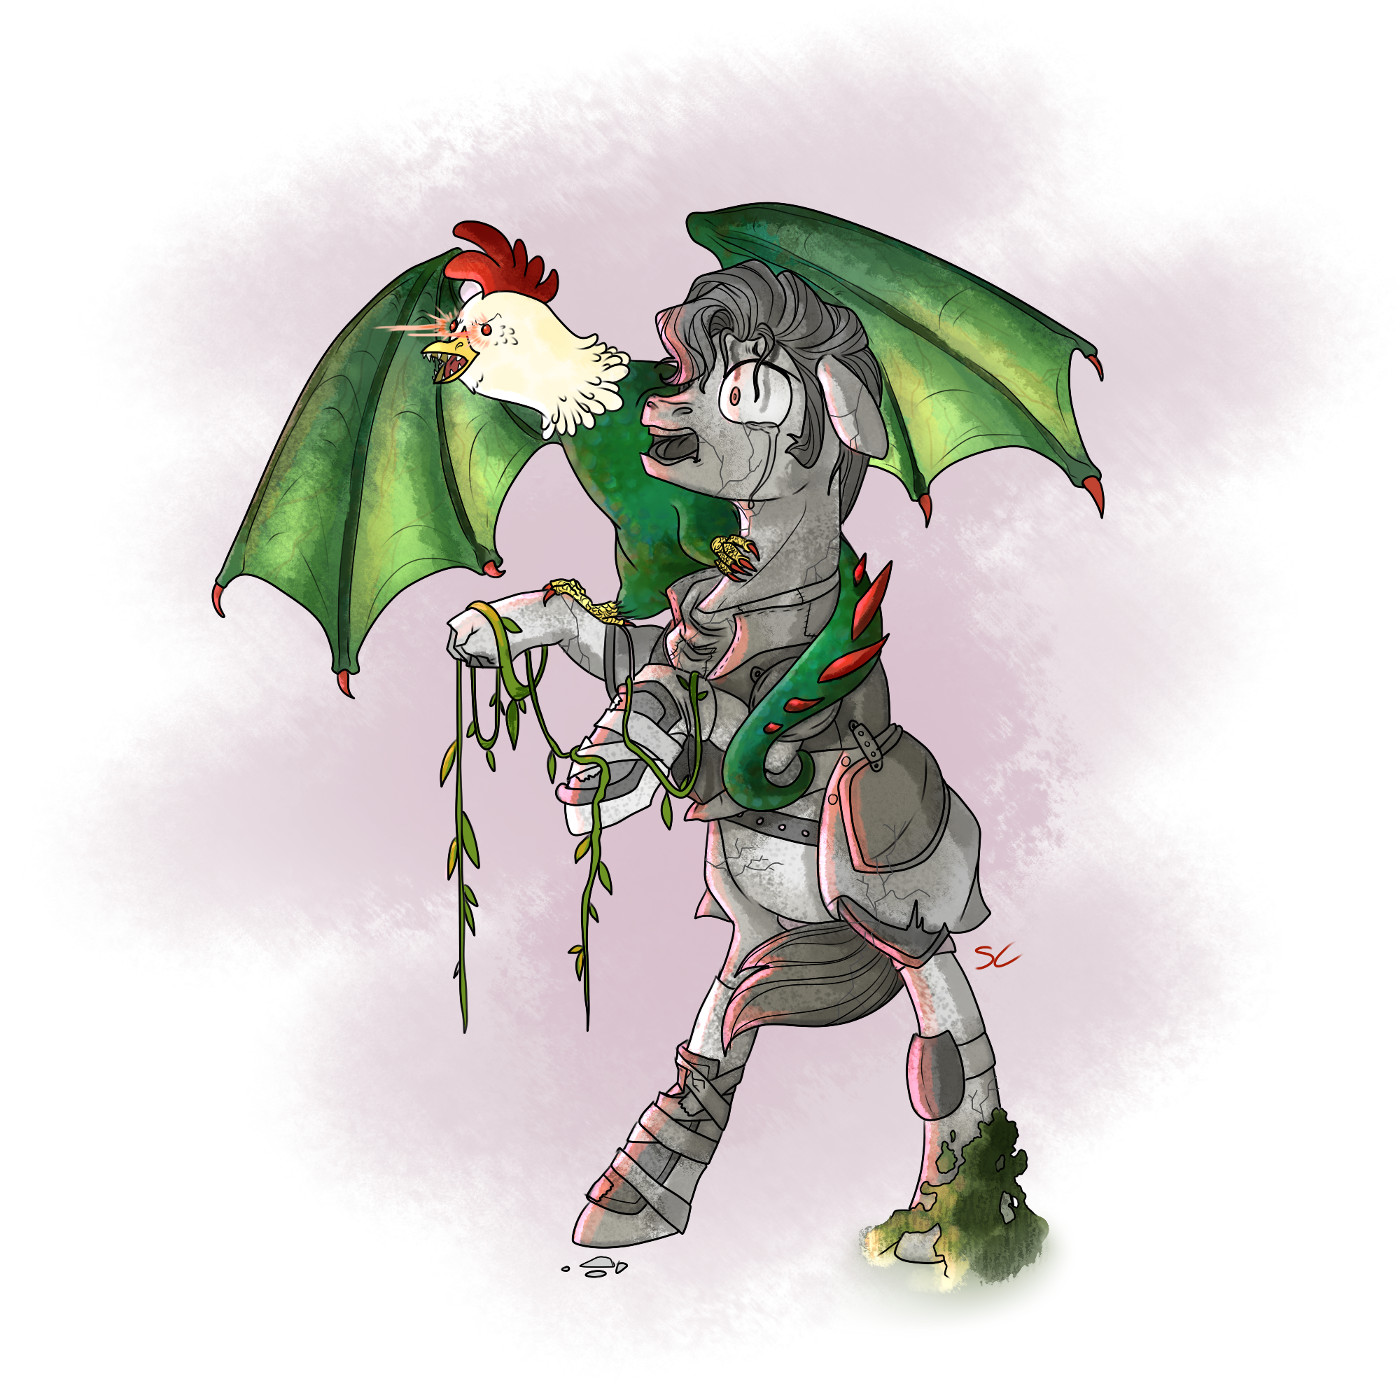
\includegraphics[width=0.7\linewidth]{ART/Enemies/Cockatrice}
	\end{figure}
	
	
	\clearpage

	\section*{Dragon}
	\addcontentsline{toc}{section}{Dragon}
	\begin{quote}
		\emph{``You want to know about dragons? Well... they're super rare, for one. And I have heard they like to collect large hoards of gems and gold. Hey, where you going...!? Come back, you'll be dead ages before you get to the dragon's hoard! ...Eh, maybe he knows what he's doing. Or maybe the dragon will roast him in his metal armor with its firebreath. That's what you get for not paying for your info.''}
	
	\emph{-	Merchant Silver Bit}
	\end{quote}
	
	\emph{\textbf{Type:} Sentient}
	
	\emph{\textbf{EXP:} 1000}
	
	{
		\rowcolors{1}{gray!30}{gray!10}
		\begin{tabu} to 150mm{| X[c,1] | X[c,1] | X[c,1] | X[c,1] | X[c,1] | X[c,1] | X[c,1] | X[c,1] |  X[c,3] | X[c,3]| X[c,3] | X[c,3] | X[c,3] |}
			\hline
			\multicolumn{13}{|c|}{\cellcolor{gray!50} Dragon Statistics}               \\ \hline
			S  & P & E & C & I & A & L & \cellcolor{gray!50} & HP & DT & AP & Size & Karma \\
			12 & 6 & 8 & 6 & 8 & 6 & 7 & \cellcolor{gray!50} & 20  & 50 & 14 & 3   & Varies   \\ \hline
		\end{tabu}
		
		%\emph{*Changeling's Karma may fluctuate depending on setting}
	}
	
	\bigskip
	{
		\rowcolors{1}{gray!30}{gray!10}
		\begin{tabu} to 150mm{| X[c,1] | X[c,1] | X[c,1] | X[c,1] | X[c,1] |}
			\hline
			\multicolumn{5}{|c|}{\cellcolor{gray!50} Skills}    \\ \hline
			Unarmed & Sneak & Diplomacy & Intimidation & Barter \\
			75      & 25    & 60        & 70           & 70     \\ \hline
		\end{tabu}
		
	}
	
	\subsubsection*{Additional Combat Details:}
	\begin{verse}
		\textbf{Firebreath (10 AP):} The notorious trait of dragons, is their ability to breath fire of immense temperatures. The firebreath can take two forms: 
		
	First form is a line of fast scorching flames, with a range of 10 meters (5 hexes). This deals 50+(6) damage, with a 2x20 \% chance of causing Burning.
	
	The second form is a fiery sphere that sets an area of Large Burst template ablaze. This area burns for 3 turns, dealing 20+(2) damage per turn, with a chance of causing Burning.
	
	\textbf{Bite (6 AP):} A mighty jaw with rows of razor sharp fangs. Deals 60 + (2) damage. Dragons have Reach of 6 meters (3 hexes).
	
	\textbf{Flying:} Dragons have working wings, thus they are capable of flight. Dragons' flight speed is 1 AP for 6 meters (3 Hexes).
	
	\textbf{Rend (6 AP):} The dragons' claws are sharp and capable of ripping apart metal and stone. The attack deals 30+(5) damage, and ignores 20 DT. Dragons have Reach of 6 meters (3 hexes).
	
	\textbf{Vanity:} Dragons can be vainglorious creatures, appeased by flattery. A target attempting to flatter a dragon gains +10 temporary bonus to Diplomacy. If the Diplomacy check fails, the following Diplomacy checks against the dragon suffers -10 instead.

	\textbf{Fire Immunity:} Dragons often use lava as a relaxing bath, and suffer no harmful effects. They're immune to Fire damage.
	
	\textbf{Poison Resistant:} Though many poisons require far larger doses to affect a dragon, they're still quite intolerant to poisons. Their poison resistance is 40.

	\textbf{Rad Resistant:} Much like ponies, dragons can go through ghoulification, and as such the un-ghoulified variant is susceptible to radiation. Their rad resistance is 40.
	\end{verse}
	
	\subsubsection*{Creature drops:}
	\begin{compactitem}
		\item Dragon Hoard; Gem (value estimated 4000 caps)
		\item Dragon Hoard; Precious item (value estimated 2000 caps)
		\item Dragon Scale (1d6+ Survival doubles u.)
		\item Dragonfire Essence (1d2+ Survival doubles u.)
	\end{compactitem}
	
	
	\subsection*{Description:}
	The mighty dragon is a sight to behold, with their strong, durable frame and thick scales that cover them from head to toe. Along with their magical dragonfire and capability to withstand intense heat, to the point that lava and firestorms are little more than a bath and a shower for them.
	
	Dragons are some of the more fearsome foes one can find, but they are sentient creatures, and as such, can be willing to negotiate. Especially if their favorite food, gemstones, are involved. However, should negotiations go awry, battle is imminent as a slighted dragon is an angry one. Then, out comes the firebreath and metal-shredding claws.
	
	Most dragons value competition and strength of individual, leaving many pony-customs of friendship and cutesy things in the dust, though this behavior is more pronounced in the young dragons. Older dragons tend to turn vain, but less aggressively macho.
	
	Dragons' size is somewhat affected by their hoards and greed needed to gather such a large collection of priceless items, gold and gems; though they do grow more naturally as well. The bigger the hoard, the larger the dragon.
	
	\bigskip
	A Dragon Lord is the ruler of the dragon, usually decided by a competition, though it may vary what kind the competition actually is. This competition is usually designed by the previous Dragon Lord, who will relinquish the symbol of their might, a Bloodstone Scepter, to the winner of the competition.
	
	Dragons are a rare sight in the Equestrian Wasteland, as they usually reside in Dragon lands, described as a barren, flat and stony plain with very little animal or plantlife.
	
	\clearpage

	\section*{Enclave}
	\addcontentsline{toc}{section}{Enclave}
	\begin{quote}
		\emph{``Well, I've only gotten to meet any of the Grand Pegasus Enclave -Snrk! Hah...!- Sorry, something in my throat, fairly recently. Lovely, lovely bunch of utter buckers, if you ask me. I have no doubt that they might have one or two good guys in them, but most of them believe the indoctrination they've been given by their government, that they're the only pure pony race due to the cloud cover having protected them from the rads... Well, you don't see  a hoof sticking out of my chest, despite me being a 4th gen Wastelander.''}
	
	\emph{-	Merchant Silver Bit}
	\end{quote}
	
	Type: Sentient
	EXP: 800
	
	{
		\rowcolors{1}{gray!30}{gray!10}
		\begin{tabu} to 150mm{| X[c,1] | X[c,1] | X[c,1] | X[c,1] | X[c,1] | X[c,1] | X[c,1] | X[c,1] |  X[c,3] | X[c,3]| X[c,3] | X[c,3] | X[c,3] |}
			\hline
			\multicolumn{13}{|c|}{\cellcolor{gray!50} Enclave Statistics}               \\ \hline
			S  & P & E & C & I & A & L & \cellcolor{gray!50} & HP & DT & AP & Size & Karma \\
			6 & 8 & 7 & 6 & 7 & 8 & 7 & \cellcolor{gray!50} & 15  & 65 & 14 & 0   & Varies   \\ \hline
		\end{tabu}
		
		%\emph{*Changeling's Karma may fluctuate depending on setting}
	}
	
	\bigskip
	{
		\rowcolors{1}{gray!30}{gray!10}
		\begin{tabu} to 150mm{| X[c,1] | X[c,1] | X[c,1] | X[c,1] | X[c,1] |}
			\hline
			\multicolumn{5}{|c|}{\cellcolor{gray!50} Skills}    \\ \hline
			MEWs & Sneak & Diplomacy & Intimidation & Barter \\
			75      & 55    & 60        & 60           & 70     \\ \hline
		\end{tabu}
		
	}
		
	\subsubsection*{Additional Combat Details:}
	\begin{verse}
			\textbf{Enclave Weaponry:} Any forces of the Enclave that come to contact with the Wasteland make a point to wear the intimidating Enclave Power Armor. This is also to shield them from the lingering radiation. In battle, Enclave soldiers use Cloud weapons nearly exclusively, as they're an Enclave design.
		
		\textbf{Purity:} Enclave is made up of pegasi exclusively, and consider other races -and groundborn pegasi- as beneath them. Enclave soldiers get a (+1) to damage when targeting other sentient races.
		
		\textbf{Organized:} The Enclave have hierarchy of leadership. They strike as units and groups of various sizes, usually under at least one commander. Eliminating such commander often leaves rest of the team at disarray and demoralized.
		
		\textbf{Poison Resistant: }Due to their sheltered life up in the clouds, a lot of the harmful toxins never reached the pegasi of the Enclave. Due to this, their Poison resistance is 5, though they can equip armor to make up for this handicap.
		
		\textbf{Rad Intolerant:} The cloudcover has kept much of the Wasteland's harms out of the pegasi lifestyle, and as such, they never grew a tolerance to the lingering radiation that other races were exposed to constantly. The Enclave's Rad Resistance is 0. Many try to shield themselves with appropriate apparel.
	\end{verse}
	
	\vfill
	\subsubsection*{Creature drops:}
	\begin{compactitem}
	\item MEW Weapon (1)
	\item MEW Ammo
	\item Armor (1)
	\item \emph{Aerodynamics Monthly} magazine (1, LCK-2 to obtain)
	\item Healing Item (1, LCK doubles u.)
	\end{compactitem}
	
	\subsection*{Description:}
	The Grand Pegasus Enclave, often referred to as Enclave for short, is a militant, technologically advanced yet somewhat secretive faction of Pegasus ponies that serves as the governing body above the clouds. They claim to be the continuation of pre-War Equestrian society, proving their point with extreme measures if need be. As such, they are extremely isolationist in nature and won't take in new members from below the cloud cover, styling anyone born below the clouds as ``a mutant'', even other pegasi. 
	
	The Enclave society is strictly regulated, following the old traditions of Pegasi culture - even from prior Equestria's time as a united nation. While highly militaristic in nature, all important decisions go through a legislative council for approval - even military campaigns.
	
	\bigskip
	The Enclave utilizes cloud weaponry in all its forms - from pistols and rifles to various cloudships. The exact nature of the scale of their weaponry is unknown, as their excursions to the Wasteland are in small numbers. 
	
	When the Enclave sends teams to the Wastes, they're well-equipped and have clear instructions on their mission - and are always accompanied by a team leader, their rank dependent on the size of the team. Their excursion to the Wasteland is for the completion of the mission only, and they won't let anyone stand in their way to its eventual success.
	
	\clearpage

	\section*{Equitron}
	\addcontentsline{toc}{section}{Equitron}
	\begin{quote}
		\emph{``Possibly the first robots that could move and... well, think. And frankly, they're not that good at that - roaming in the ruins where they were left, doing the same tasks that were programmed into their arcana-drives by their masters long gone. Actually, that `thinking' part might be overestimating their capabilities...''}
	
	\emph{-	Scribe Star Twinkle}
	\end{quote}
	
	\emph{\textbf{Type:} Machine}
	
	\emph{\textbf{EXP:} 150}
	
	{
		\rowcolors{1}{gray!30}{gray!10}
		\begin{tabu} to 150mm{| X[c,1] | X[c,1] | X[c,1] | X[c,1] | X[c,1] | X[c,1] | X[c,1] | X[c,1] |  X[c,3] | X[c,3]| X[c,3] | X[c,3] | X[c,3] |}
			\hline
			\multicolumn{13}{|c|}{\cellcolor{gray!50} Equitron Statistics}                  \\ \hline
			S & P & E & C & I & A & L & \cellcolor{gray!50} & HP & DT & AP & Size & Karma  \\
			8 & 5 & 6 & 3 & 3 & 4 & 4 & \cellcolor{gray!50} & 7 & 20 & 10 & 0    & 0 \\ \hline
		\end{tabu}
		
		%\emph{*Changeling's Karma may fluctuate depending on setting}
	}
	
	\bigskip
	{
		\rowcolors{1}{gray!30}{gray!10}
		\begin{tabu} to 150mm{| X[c,1] | X[c,1] | X[c,1] | X[c,1] |}
			\hline
			\multicolumn{4}{|c|}{\cellcolor{gray!50} Skills} \\ \hline
			Firearms & MEWs & Melee & Unarmed                \\
			50       & 50   & 50    & 50                     \\ \hline
		\end{tabu}
		
	}
	
	\subsubsection*{Additional Combat Details:}
	\begin{verse}
		\textbf{Laser Beam (4 AP):} Equitrons are outfitted with a \emph{Q-Same AEW-21 Arcane Rifle}, dealing 15+(1) damage and ignoring 5 DT.
		
	\textbf{Cutter (4 AP):} Equitrons are outfitted with a Ripper, and deal damage accordingly, in Equitron's case 40+(4).
	
	\textbf{Riot control (4 AP):} If an Equitron successfully grapples someone, they may cause a Stun-status effect with an END roll to resist.
	
	\textbf{Slow:} Equitrons have slower ground movements than most ponies due to their mechanical but rigid legs, giving them movement speed of 2 AP per 2 meters (1 hexes.)
	
	\textbf{Self-destruct:} Upon reaching 0 HP, Equitron explodes with a Small Burst template centered on itself. Deals 50 + (2) damage.
	
	\textbf{Combat Inhibitor:} Equitrons are equipped with a combat inhibitor, that help them separate friends from woes. Combat inhibitor can be hacked with Science to various ends, such as shutting down the Equitron. Destroying the combat inhibitor turns Equitron against anything around them. 
	
	\textbf{Painless:} As a machine, Equitron has no Pain Thresholds.
	
	\textbf{Poison Immunity:} As a machine, Equitron is immune to toxins.
	
	\textbf{Rad Immunity:} Due to not being alive, radiation has no effect on Equitron.
	\end{verse}
	
	\subsubsection*{Creature drops:}
	\begin{compactitem}
		\item Scrap Electronics (1d2+Mechanics doubles u.)
		\item Scrap Metal (1d4+Mechanics doubles u.)
		\item Magical Energy Rifle (1)
		\item Ripper (1)
	\end{compactitem}
		
	\subsection*{Description:}
	Equitrons are four-legged mechanical beings that resemble their creators loosely. Slow and cumbersome, these robotic ponies may have easily been surpassed later down the line with an improved model if it were not for the Great War. However, they're reliable and programmed to specific tasks, thus making them ideal in many scenarios, both pre- and post-War.
	
	Equitrons are noted to be the first moving robots, and are very sturdy as a result. Their original development cause by Robronco has been forgotten, but a myriad of models exist based on the same base model - be it construction, peacekeeping, or monorail ticket inspector role. They're very strictly programmed - thus working against the robot's instructions may incur its wrath and pacifying protocols. An expert mechanic may tweak the robot's parameters to more of their liking, and a skilled hacker may reprogram the robot from a linked terminal.
	
	\bigskip
	Given the myriad of roles it was assigned for, one can easily find Equitrons almost anywhere where there has been ponies, most often within urban centers. Due to their programming, they hardly wander off of their designated areas. And when they do, they're certainly glitchy in coding and hostile in attitude.
	
	\clearpage

	\section*{Feral Dog}
	\addcontentsline{toc}{section}{Feral Dog}
	\begin{quote}
		\emph{``Not exactly your garden variety of Fido, they're the descendants of the countless dogs that remained after the war, fighting for survival. Hence why they're not truly wild, and can, with patience, be tamed. Just... takes a lot of time and effort. And bites, lots of bites. That's really all they do, try to go for the jugular.''}
	
	\emph{-	Verdant Brink, Hunter}
	\end{quote}
	
	\emph{\textbf{Type:} Mutated Animal}
	
	\emph{\textbf{EXP:} 50}
	
	{
		\rowcolors{1}{gray!30}{gray!10}
		\begin{tabu} to 150mm{| X[c,1] | X[c,1] | X[c,1] | X[c,1] | X[c,1] | X[c,1] | X[c,1] | X[c,1] |  X[c,3] | X[c,3]| X[c,3] | X[c,3] | X[c,3] |}
			\hline
			\multicolumn{13}{|c|}{\cellcolor{gray!50} Feral Dog Statistics}                  \\ \hline
			S & P & E & C & I & A & L & \cellcolor{gray!50} & HP & DT & AP & Size & Karma  \\
			7 & 4 & 6 & 3 & 1 & 8 & 4 & \cellcolor{gray!50} & 6 & 0 & 14 & -1    & 0 \\ \hline
		\end{tabu}
		
		%\emph{*Changeling's Karma may fluctuate depending on setting}
	}
	
	\bigskip
	{
		\rowcolors{1}{gray!30}{gray!10}
		\begin{tabu} to 60mm{| X[c,1] | X[c,1] |}
			\hline
			\multicolumn{2}{|c|}{\cellcolor{gray!50} Skills} \\ \hline
			Unarmed & Sneak                                  \\
			45      & 55                                     \\ \hline
		\end{tabu}
		
	}
	
	\subsubsection*{Additional Combat Details:}
	\begin{verse}
		\textbf{Bite (3 AP):} Feral dogs try to use their natural weapons, jaws, to take down creatures. The attack deals 10+(3) damage, and can cause a Bleeding-status effect.
		
		\textbf{Quick Runner:} Due to their nimble bodies, Feral Dogs gain +2 to initiative rolls.
		
		\textbf{Pack Hunters:} Feral dogs travel mostly in packs, and strike as a force to bring down their prey. When two or more feral dogs attack same target, they get +10 to Trip attempts.
	
		\textbf{Poison Resistant:} Feral dogs are rather sickly creatures, thus having a poison resistance of 10.
		
		\textbf{Rad Resistant:} Feral dogs have gotten accustomed to all the background radiation, giving them a Rad resistance of 15.
	\end{verse}
	
	\subsubsection*{Creature drops:}
	Dog Meat (1-4 pieces, Survival doubles u.)
	
	\vfill
	\subsection*{Feral Mongrel}
	\addcontentsline{toc}{subsection}{Feral Mongrel}
	\begin{quote}
		\emph{``Feral Mongrel is the ghoulified variant of a feral dog, usually found skulking about in highly irradiated areas. They're a little tougher than a regular dog, and they seem to prefer the company of other ghoul creatures. So don't be surprised if a few mongrels tag along a feral or some sane ghoul, seems even after ghoulification they're determined to be a ghoul's best friend.''}
	
	\emph{-	Star Paladin Glitter Dust}
	\end{quote}
	
	\emph{\textbf{Type:} Abomination}
	
	\emph{\textbf{EXP:} 50}
	
	{
		\rowcolors{1}{gray!30}{gray!10}
		\begin{tabu} to 150mm{| X[c,1] | X[c,1] | X[c,1] | X[c,1] | X[c,1] | X[c,1] | X[c,1] | X[c,1] |  X[c,3] | X[c,3]| X[c,3] | X[c,3] | X[c,3] |}
			\hline
			\multicolumn{13}{|c|}{\cellcolor{gray!50} Feral Mongrel Statistics}                  \\ \hline
			S & P & E & C & I & A & L & \cellcolor{gray!50} & HP & DT & AP & Size & Karma  \\
			7 & 4 & 6 & 3 & 2 & 8 & 4 & \cellcolor{gray!50} & 9 & 5 & 14 & -1    & 0 \\ \hline
		\end{tabu}
		
		%\emph{*Changeling's Karma may fluctuate depending on setting}
	}
	
	\bigskip
	{
		\rowcolors{1}{gray!30}{gray!10}
		\begin{tabu} to 60mm{| X[c,1] | X[c,1] |}
			\hline
			\multicolumn{2}{|c|}{\cellcolor{gray!50} Skills} \\ \hline
			Unarmed & Sneak                                  \\
			55      & 60                                     \\ \hline
		\end{tabu}
		
	}
	
	\subsubsection*{Additional Combat Details:}
	\begin{verse}
		\textbf{Bite (3 AP):} Feral Mongrels try to use their natural weapons, jaws, to take down creatures. The attack deals 10+(3) damage, and can cause a Bleeding-status effect.
	
	\textbf{Glowing Lick (5 AP):} Feral Mongrels have irradiated saliva, and generally tend to be rather sloppy. Their saliva, which they deliver with fierce licking of target, deals 1 Rad on 1x40\% chance.
	
	\textbf{Quick Runner:} Due to their nimble bodies, Feral mongrels gain +2 to initiative rolls.
	
	\textbf{Pack Hunters:} Feral mongrels travel mostly in packs, and strike as a force to bring down their prey. When two or more feral dogs attack same target, they get +10 to Trip attempts.
	
	\textbf{Poison Resistant:} Feral mongrel are rather sickly creatures, thus having a poison resistance of 10.
	
	\textbf{Rad Resistant:} Feral mongrels have developed a much stronger Rad Resistance of 50, than the normal dogs.
	\end{verse}
	
	\subsubsection*{Creature drops:}
	\begin{compactitem}
		\item Mongrel Meat (Abomination flesh piece 1d2+Survival doubles u.)
		\item Mongrel Saliva (Irradiated Material 1+Survival doubles u.)
	\end{compactitem}

	\subsection*{Description:}
	Dogs, the canine friends of ponies, did weather the destructive end of the world like their masters. Most that survived and were left without their owners quickly learned the harsh truth of the wasteland, turning them to their feral, untamed ways. 
	
	Feral dogs can be seen roaming almost anywhere in the wastes. No spot is too strange for them, and with a large pack they can claim any ruin as their home. They do have a tendency to steer clear from heavily robotically guarded buildings, for they cannot down the mechanical beasts with ease.
	
	\bigskip
	Feral dogs can appear alone, but most often one can find them in groups of 2-4, depending on location. They tend to rush to a target, aiming for the throat to take the target down as quickly as possible. However, unless they manage to catch one unawares, they're relatively easy to fend off.
	
	These dogs can, and often have been tamed, but it has sometimes taken a few generations' worth of feral dogs to bring back the companion many ponies know and love. These dogs are often bred and sold as companions to all. Some raise them to be attack and guard dogs, while others prefer a calmer companion for their daily tasks. 
	
	\bigskip
	Feral Mongrels behave much in the same way, with the only exception to the feral dog being their irradiated, pale and hairless skin and slightly more intelligent behavior. Feral dogs and Feral mongrels rarely mix, preferring to have their own, separate packs.
	
	\clearpage

	\section*{Feral Ghoul}
	\addcontentsline{toc}{section}{Feral Ghoul}
	\begin{quote}
			\emph{``The ever-popular zombie of the Wastes. What remains of a mutated pony after they've went a bit too soft in the head. Unfortunately for you, they're vicious, fast and they really want to tear your face off. So Initiate, better have that rifle ready, because they won't wait for you to pull it out. They're radioactive as well, so hope you packed enough Rad-Away.''}
		
		\emph{-	Star Paladin Glitter Dust}
	\end{quote}
	
	\emph{\textbf{Type:} Abomination}
	
	\emph{\textbf{EXP:} 100}
	
	{
		\rowcolors{1}{gray!30}{gray!10}
		\begin{tabu} to 150mm{| X[c,1] | X[c,1] | X[c,1] | X[c,1] | X[c,1] | X[c,1] | X[c,1] | X[c,1] |  X[c,3] | X[c,3]| X[c,3] | X[c,3] | X[c,3] |}
			\hline
			\multicolumn{13}{|c|}{\cellcolor{gray!50} Feral Ghoul Statistics}           \\ \hline
			S & P & E & C & I & A & L & \cellcolor{gray!50} & HP & DT & AP & Size & Karma \\
			5 & 6 & 5 & 2 & 1 & 7 & 4 & \cellcolor{gray!50} & 12 & 0  & 13 & 0    & 0     \\ \hline
		\end{tabu}
		
		%\emph{*Changeling's Karma may fluctuate depending on setting}
	}
	
	\bigskip
	{
		\rowcolors{1}{gray!30}{gray!10}
		\begin{tabu} to 60mm{| X[c,1] | X[c,1] |}
			\hline
			\multicolumn{2}{|c|}{\cellcolor{gray!50} Skills} \\ \hline
			Unarmed & Sneak                                  \\
			40      & 50                                     \\ \hline
		\end{tabu}
		
	}

	\subsubsection*{Additional Combat Details:}
	\begin{verse}
		\textbf{Irradiated Hoof (5 AP):} Feral ghoul's hoof-strike deals 10 + (3) damage, and gives 1 Rad Token at 2x50\% chance.
	
	\textbf{Rad Healing (1/min, 8 AP):} The ghoul may choose to discard 2-5 Rad Tokens, and replenish an equal amount of lost HP and/or Crippled Conditions, if any are present.
	
	\textbf{Quick Runner:} Feral Ghouls are fast, and due to this they get a +2 to their Initiative rolls.
	
	\textbf{Pain Tolerance:} Due to their fervor with which they attack, Ferals have learned to ignore pain. Feral Ghouls' Pain Thresholds begin from 3-2 and 1, rather than starting from 5-4.

	\textbf{Instinct:} Feral Ghoul unicorns, griffins and Pegasi are able to use their innate magic, though in limited ways. Unicorns have General school spells available to them, while griffins and pegasi can take to the air and fly towards their targets.

	\textbf{Poison Resistance:} Ghouls still retain the natural Poison Resistance of the Equines and Griffons they were, thus having Poison Resistance of 10 (20 if they are Zebras). 
	\end{verse}
	
	\subsubsection*{Creature drops:}
	\begin{compactitem}
		\item Ghoul Flesh (Abomination flesh piece 1d2+Survival doubles u.)
		\item Junk (1d6)
		\item Random Clothing or Armor in Poor Condition (1 u.)
		\item Caps (1d12, LCK doubles u.)
	\end{compactitem}
	
	\subsection*{Glowing One}
	\addcontentsline{toc}{subsection}{Glowing One}
	\begin{quote}
		\emph{``If you thought the regular old Feral was annoying to deal with, take a load of this. Glowing One. It behaves much like other ghouls, but it is irradiated so badly that it radiates. As you can probably guess from the name. They can also release this radiation at you with a burst, so stay away from them. You'll get sick in no time.''}
	
	\emph{-	Star Paladin Glitter Dust}
	\end{quote}
	
	\emph{\textbf{Type:} Abomination}
	
	\emph{\textbf{EXP:} 200}
	
	{
		\rowcolors{1}{gray!30}{gray!10}
		\begin{tabu} to 150mm{| X[c,1] | X[c,1] | X[c,1] | X[c,1] | X[c,1] | X[c,1] | X[c,1] | X[c,1] |  X[c,3] | X[c,3]| X[c,3] | X[c,3] | X[c,3] |}
			\hline
			\multicolumn{13}{|c|}{\cellcolor{gray!50} Glowing One Statistics}           \\ \hline
			S & P & E & C & I & A & L & \cellcolor{gray!50} & HP & DT & AP & Size & Karma \\
			6 & 6 & 7 & 3 & 2 & 7 & 4 & \cellcolor{gray!50} & 15 & 10  & 13 & 0    & 0     \\ \hline
		\end{tabu}
		
		%\emph{*Changeling's Karma may fluctuate depending on setting}
	}
	
	\bigskip
	{
		\rowcolors{1}{gray!30}{gray!10}
		\begin{tabu} to 60mm{| X[c,1] | X[c,1] |}
			\hline
			\multicolumn{2}{|c|}{\cellcolor{gray!50} Skills} \\ \hline
			Unarmed & Sneak                                  \\
			70      & 70                                     \\ \hline
		\end{tabu}
		
	}
		
	\subsubsection*{Additional Combat Details:}
	\begin{verse}
		\textbf{Irradiated Hoof (5 AP):} Feral ghoul's hoof-strike deals 10 + (5) damage, and gives 1 Rad Token at 2x60\% chance.
	
		\textbf{Rad Healing (1/min, 8 AP):} The ghoul may choose to discard 2-5 Rad Tokens, and replenish an equal amount of HP tokens and/or Crippled Conditions, if any are present.

		\textbf{Irradiated Burst (1/min, 8 AP):} Having soaked up radiation, the Glowing One can expel Rads in a burst around it, in a Medium Burst area centered on the ghoul. This attack gives 1 Rad Token at 5x50\% chance.

		\textbf{Irradiated Presence:} Merely by staying close to a Glowing One, does their irradiated body endanger, or revitalize those in their proximity. Each turn spent within a Tiny Burst area around the Glowing one gives 1 Rad Token at 1 x 40 \% chance.

		\textbf{Quick Runner:} Feral Ghouls are fast, and due to this they get a +2 to their Initiative rolls.

		\textbf{Pain Tolerance:} Due to their fervor with which they attack, Ferals have learned to ignore pain. Feral Ghouls' Pain Thresholds begin from 3-2 and 1, rather than starting from 5-4.

		\textbf{Instinct:} Feral Ghoul unicorns, griffins and Pegasi are able to use their innate magic, though in limited ways. Unicorns have General school spells available to them, while griffins and pegasi can take to the air and fly towards their targets.

		\textbf{Poison Resistance:} Ghouls still retain the natural Poison Resistance of the Equines and Griffons they were, thus having Poison Resistance of 10 (20 if they are Zebras).
	\end{verse}
	
	\subsubsection*{Creature drops:}
	\begin{compactitem}
		\item Glowing Flesh (Irradiated material 1d2+ Survival doubles u.)
		\item Random Skill Magazine (1, LCK-2 to obtain)
		\item Junk (1d6)
	\end{compactitem}
	
	\subsection*{Description:}
	
	\begin{wrapfigure}{R}{0pt}
		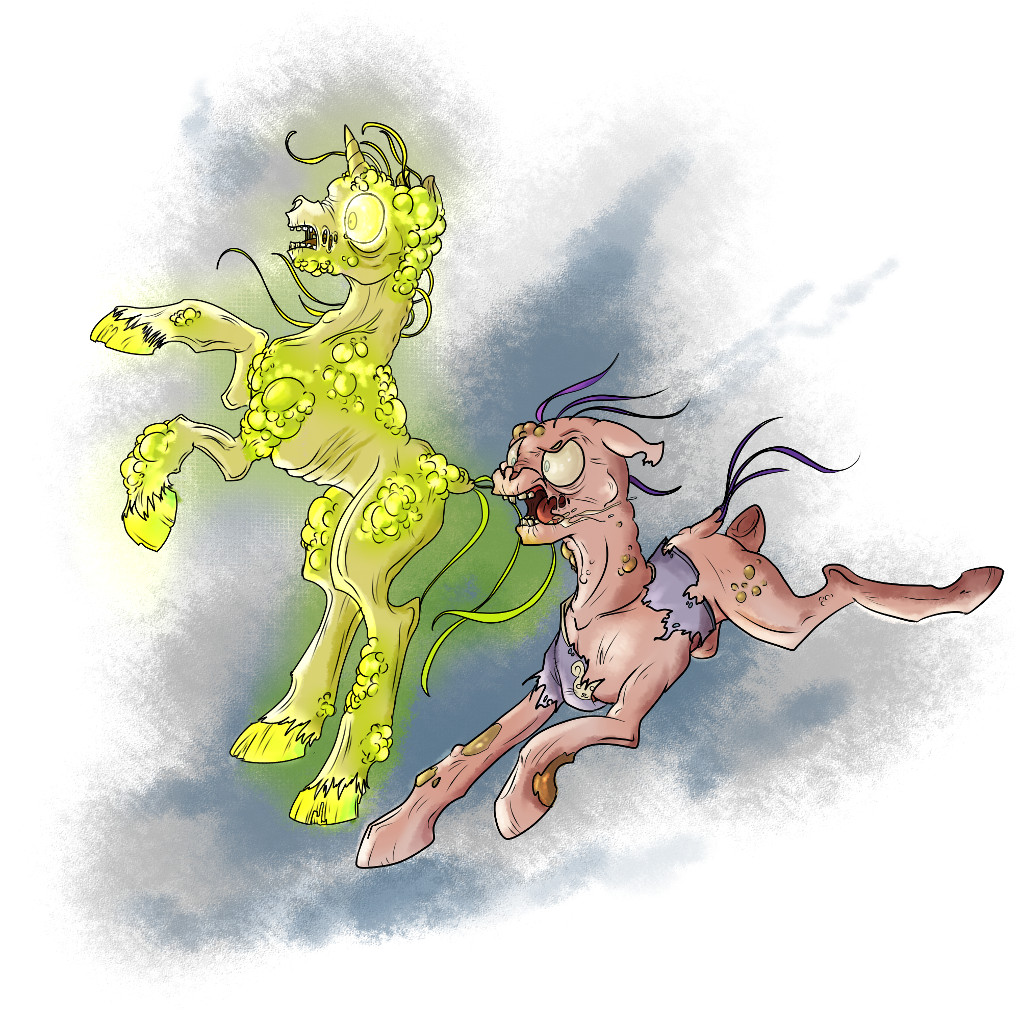
\includegraphics[width=0.5\linewidth]{ART/Enemies/ghoul}
	\end{wrapfigure}
	
	While turning into a ghoul provides one with the benefits of longevity, sometimes the age will catch up on the ghouls. Or some other trauma made them lose their minds, turning them to the feral state. While still capable of basic instincts, the feral ghouls differ from their non-feral cousins in that they no longer think rationally, being closer to animals with their sentience.
	
	Feral ghouls gather together in small packs, preferring dark and cool environments to call their little base - like basements or underground passageways. They do not, however, fear light as some may think, perfectly capable of wandering the wasteland. Occasionally they gather in  irradiated areas, as they note the restorative effects of the fallout - as with normal ghouls, not only feral ghouls do not suffer negative effects from radiation, they are practically healed by it. 
	
	\bigskip
	Feral ghouls do not create complex plans of attack - they tend to swarm any intruder they spot, usually alerting their pack with a scream for additional power before charging. They do, however, retain some memories of their old life, and usually use the skills and tactics they have learned in occasion - often helping the feral pack as a whole.
	
	Glowing ones are special ghouls, having become conduits of radiation themselves. They emit this radiation around them, and occasionally shed it in large bursts around them - effectively healing their ghoul friends.  
	
	\clearpage

	\section*{Fire Ant}
	\addcontentsline{toc}{section}{Fire Ant}
	\begin{quote}
		\emph{``So, the biological weapon we were asked to engineer for MoA... I call it the Fire Ant. I know, not the most original of names, but I'm a scientist, not an artist. It can spew burning liquid at least four meters in length and they're huge! Who knew I.M.P had such wonderful properties? Now if only I could get in contact with MoA...''}
	
	\emph{-	Acacia Honey, Entomologist}
	\end{quote}
	
	
	\emph{\textbf{Type:} Mutated Insect}
	
	\emph{\textbf{EXP:} 100}
	
	{
		\rowcolors{1}{gray!30}{gray!10}
		\begin{tabu} to 150mm{| X[c,1] | X[c,1] | X[c,1] | X[c,1] | X[c,1] | X[c,1] | X[c,1] | X[c,1] |  X[c,3] | X[c,3]| X[c,3] | X[c,3] | X[c,3] |}
			\hline
			\multicolumn{13}{|c|}{\cellcolor{gray!50} Fire Ant Statistics}             \\ \hline
			S & P & E & C & I & A & L & \cellcolor{gray!50} & HP & DT & AP & Size & Karma \\
			6 & 5 & 6 & 3 & 2 & 7 & 5 & \cellcolor{gray!50} & 10 & 15 & 13 & -1   & 0     \\ \hline
		\end{tabu}
		
		%\emph{*Changeling's Karma may fluctuate depending on setting}
	}
	
	\bigskip
	{
		\rowcolors{1}{gray!30}{gray!10}
		\begin{tabu} to 60mm{| X[c,1] | X[c,1] |}
			\hline
			\multicolumn{2}{|c|}{\cellcolor{gray!50} Skills} \\ \hline
			Unarmed & Sneak                                  \\
			70      & 60                                     \\ \hline
		\end{tabu}
		
	}
	
	\subsubsection*{Additional Combat Details:}
	\begin{verse}
		\textbf{Pincers (8 AP):} Fire Ants will try to bite and rip ponies legs off with force. This attack deals 20+(3) damage. The attack has 10\% base chance of causing Crippled status, with each removed HP token adding 10\% to this chance.
	
		\textbf{Firebreath (1/min, 6 AP):} Fire Ants can spray a burning liquid with a range of 4/8/16 on a Small Burst template. This attack deals 10+(4) of damage, with a chance of causing Burning. This fire stays lit for 3 turns.

		\textbf{Territorial:} Fire Ants will defend their nests ferociously and with great numbers.

		\textbf{Insect Brain:} Crippling the Fire Ant's antennae causes the Ant to gain Mind Controlled and Enraged -status effects and make them attack the nearest creature, be it friend or foe.
	\end{verse}
	
	\subsubsection*{Creature drops:}
	Ant Nectar (1-2+ Survival doubles u.)
	
	\vfill
	
	\subsection*{Fire Ant Queen}
	\addcontentsline{toc}{subsection}{Fire Ant Queen}
	\begin{quote}
		\emph{``The fire ant queen was a resounding success! Only after three tries of dipping them in I.M.P. it has generated the desired traits without defects like dying on the spot. And it seems to keep its wings well after mating too... This is fantastic, they can assist the pegasi in air-raids with their firebreath!''}

	\emph{-	Acacia Honey, Entomologist}
	\end{quote}
	
	\emph{\textbf{Type:} Mutated Insect}
	
	\emph{\textbf{EXP:} 250}
	
	{
		\rowcolors{1}{gray!30}{gray!10}
		\begin{tabu} to 150mm{| X[c,1] | X[c,1] | X[c,1] | X[c,1] | X[c,1] | X[c,1] | X[c,1] | X[c,1] |  X[c,3] | X[c,3]| X[c,3] | X[c,3] | X[c,3] |}
			\hline
			\multicolumn{13}{|c|}{\cellcolor{gray!50} Fire Ant Statistics}                \\ \hline
			S & P & E & C & I & A & L & \cellcolor{gray!50} & HP & DT & AP & Size & Karma \\
			7 & 5 & 7 & 2 & 2 & 8 & 5 & \cellcolor{gray!50} & 15 & 25 & 13 & 3    & 0     \\ \hline
		\end{tabu}
		
		%\emph{*Changeling's Karma may fluctuate depending on setting}
	}
	
	\bigskip
	{
		\rowcolors{1}{gray!30}{gray!10}
		\begin{tabu} to 60mm{| X[c,1] | X[c,1] |}
			\hline
			\multicolumn{2}{|c|}{\cellcolor{gray!50} Skills} \\ \hline
			Unarmed & Sneak                                  \\
			70      & 70                                     \\ \hline
		\end{tabu}
		
	}
	
	\subsubsection*{Additional Combat Details:}
	\begin{verse}
		\textbf{Pincers (8 AP):} Fire Ants will try to bite and rip ponies legs off with force. This attack deals 50+(3) damage. The attack has 10\% base chance of causing Crippled status, with each removed HP token adding 10\% to this chance.
	
		\textbf{Firebreath (1/min, 6 AP):} Fire Ants can spray a burning liquid with a range of 8/16/32 on a Small Burst template. This attack deals 20+(4) of damage, with a chance of causing Burning with -1 END to resist.
	
		\textbf{Sweep (4 AP):} Fire Ant Queen can make a sweeping motion with its first pair of legs. This attack deals 20+(2) damage and as a 10\% chance to trip a target.
	
		\textbf{Reach:} Fire ant queens have a reach of 4 meters / 2 hexes.
	
		\textbf{Flight:} Fire ant queens have working wings, which they use well. Their flight speed is 1 AP for 2 meters/1 hex.
	
		\textbf{Insect Brain:} Crippling the Fire Ant?s antennae causes the Ant to gain Mind Controlled and Enraged -status effects and make them attack the nearest creature, be it friend or foe.
	\end{verse}

	
	\subsubsection*{Creature drops:}
	\begin{compactitem}
		\item Ant Nectar (1d4+ Survival doubles u.)
		\item Ant Pheromones (1+Survival doubles u.)
	\end{compactitem}
	
	\vfill
	\subsection*{Description:}
	Fire ants are, by comparison, more aggressive and magical counterpart of the giant ant. Developed from another ant species intentionally, it possesses abilities that giant ants do not have: ability to breathe fire.
	
	Easily recognizable from their red and orange color scheme, these vicious creatures do not make the slightest attempt to blend in, relying on both strength of numbers and their firebreath to singe everything they deem an obstacle. Once they enter an area, they will dedicate all of their power to build a nest -usually a large mound partially underground- and then eradicate all competition from the area. Due to this, it is rare to see different insects in an area with a large colony of fire ants.
	
	\bigskip
	Fire ants do usually use their firebreath only to fend for themselves, to keep safe distance from their enemy. For prey, mandibles are usually deemed good enough. The fire ants include much in their menu, including other insects such as radroaches and giant ants to brahmin, geckoes and jackalopes. They also include Cockatrice in their natural diet, as they are immune to Cockatrice's stone-turning stare, likely derived from their I.M.P. dip.
	
	Fire ant queens are different from giant ant queens in that they retain their wings even after birthing a colony's worth of workers and soldiers. This means that this highly aggressive mama can and will pursue their offender if other defenses for the nest fails. And much like any angry mother, she is relentless in her pursuit.
	
	\begin{figure}
		\centering
		\includegraphics[width=0.8\linewidth]{"ART/Enemies/Fire ant"}
	\end{figure}
	
	
	\clearpage

	\section*{Firebush}
	\addcontentsline{toc}{section}{Firebush}
	\begin{quote}
		\emph{``Originally from the bayou, this mutated plant spits out its seed pods at anything it senses moving by. These seed pods contain both seeds and a highly flammable oil, that upon exploding on the victim's face or body, reacts with air and sets ablaze immediately, giving the seeds a nice, ashy earth to sprout from. Unfortunately, it is a very large bush... but thankfully, it's range isn't terribly long. Nevertheless, nasty burns are in your future.''}
	
	\emph{-	Doc Holly}
	\end{quote}
	Type: Mutated Plant
	EXP: 50

	{
		\rowcolors{1}{gray!30}{gray!10}
		\begin{tabu} to 150mm{| X[c,1] | X[c,1] | X[c,1] | X[c,1] | X[c,1] | X[c,1] | X[c,1] | X[c,1] |  X[c,3] | X[c,3]| X[c,3] | X[c,3] | X[c,3] |}
			\hline
			\multicolumn{13}{|c|}{\cellcolor{gray!50} Firebush Statistics}                \\ \hline
			S & P & E & C & I & A & L & \cellcolor{gray!50} & HP & DT & AP & Size & Karma \\
			4 & 7 & 6 & 3 & 1 & 4 & 6 & \cellcolor{gray!50} & 12 & 10 & 12 & 1    & 0     \\ \hline
		\end{tabu}
		
		%\emph{*Changeling's Karma may fluctuate depending on setting}
	}
	
	\bigskip
	{
		\rowcolors{1}{gray!30}{gray!10}
		\begin{tabu} to 60mm{| X[c,1] | X[c,1] |}
			\hline
			\multicolumn{2}{|c|}{\cellcolor{gray!50} Skills} \\ \hline
			Unarmed & Melee                                  \\
			60      & 60                                     \\ \hline
		\end{tabu}
		
	}

	\subsubsection*{Additional Combat Details:}
	\begin{verse}
		\textbf{Seed Burst (6 AP):} Firebush spits out its seed pods (Melee, range 10/20/40), coated in a flammable oils that explode upon contact. The attack deals 30+(1) Fire damage, and can cause a Burning-status effect.
	
	\textbf{Immobile:} Firebush are rooted in place, so they have no movement speeds. 
	
	\textbf{Cold Weakness:} Firebushes are weak against Cold and Cold-based damage. Firebushes take double the damage against Cold and Cold-based damage.
	
	\textbf{Fire Resistant:} Firebushes have naturally higher DT against Fire damage. They gain +40 DT against Fire damage.
	
	\textbf{Poison Resistant:} As plants, Firebushes are immune to poisons other than herbicides. Against herbicides, Firebushes have poison resistance of 20.
	
	\textbf{Rad Resistant:} As Firebushes are radiation mutated plants, their high Rad Resistance allows them to bloom in highly radiated areas. Their Rad Resistance is 50.
	\end{verse}
	
	\subsubsection*{Creature drops:}
	\begin{compactitem}
		\item Firebush Oil (1+Survival doubles u.)
		\item Firebush Seed Pod (1d4 with Survival)
		\item Red Herbs (1d4+Survival doubles u.)
	\end{compactitem}
	
	\subsection*{Description:}
	Firebush is a large plant that mostly inhabits marshes and wetlands. As it is a plant, it doesn't act with vindictive manner, mostly targeting moving creatures for the sake of spreading its seeds. The firebush requires an ashen ground to sprout properly and the plant has evolved with its mutations to ensure that. The seed pods contain a flammable oil that sets ablaze the moment it comes into contact with air when the fragile shell of the seed pod breaks. This chemical reaction causes an explosion that can be fatal. However, this is the plant's only harmful effect. In fact, the plant in question is downright harmless when the seeds have not developed yet.
	
	If one is able to collect the seed pods without breaking them, they can be made into makeshift bombs.
	
	\begin{figure}[h]
		\centering
		\includegraphics[width=0.7\linewidth]{"ART/Enemies/firebush"}
	\end{figure}
	
	\clearpage
	
	\section*{Flash Bee}
	\addcontentsline{toc}{section}{Flash Bee}
	\begin{quote}
		\emph{``Originally the Flash Bee has inhabited mostly bogs and swamps, but after the war it spread far further, and their nests are far more common sight in the Wastes. Their nests are rarely seen close to urban areas, having an aversion to being bothered. If bothered, they attack viciously.''}
		
		\emph{-	Acacia Honey, Entomologist}
	\end{quote}
	
	\emph{\textbf{Type:} Non-Mutated Insect}
	
	\emph{\textbf{EXP:} 200}
	
	{
		\rowcolors{1}{gray!30}{gray!10}
		\begin{tabu} to 150mm{| X[c,1] | X[c,1] | X[c,1] | X[c,1] | X[c,1] | X[c,1] | X[c,1] | X[c,1] |  X[c,3] | X[c,3]| X[c,3] | X[c,3] | X[c,3] |}
			\hline
			\multicolumn{13}{|c|}{\cellcolor{gray!50} Twittermite Statistics}                  \\ \hline
			S & P & E & C & I & A & L & \cellcolor{gray!50} & HP & DT & AP & Size & Karma \\
			3 & 8 & 4 & 3 & 2 & 8 & 5 & \cellcolor{gray!50} & 10 & 10 & 12 & -3   & 0     \\ \hline
		\end{tabu}
		
		%\emph{*See Additional Combat Details}
	}
	
	\bigskip
	{
		\rowcolors{1}{gray!30}{gray!10}
		\begin{tabu} to 60mm{| X[c,1] | X[c,1] |}
			\hline
			\multicolumn{2}{|c|}{\cellcolor{gray!50} Skills} \\ \hline
			Unarmed & Sneak                                  \\
			60      & 30                                     \\ \hline
		\end{tabu}
		
	}
	
	\subsubsection*{Additional Combat Details:}
	\begin{verse}
		\textbf{Shock Stinger (4 AP):} Flash Bees? main method of attacking is to aggressively sting anything that it can reach. Their stinging deals 30+(2) electric damage and can cause Stun -Status effect. Targets of this attack can resist with an $END+1$ roll.
		
		\textbf{Swarm o' Bees:} Flash Bees cover an area equal to Small Burst Template. They can move to an occupied hex, and can attack any creature within said area for the cost of one attack. Due its large size of swarm, explosives and other similar Area of Effect attacks consider Flash Bees to be Size 0.
		
		\textbf{Quick Flier:} Flash Bees are fast, and due to this they get a +2 to their Initiative rolls.
		
		\textbf{Flying:} Flash Bees move by flight, moving with erratic movements. Their flight speed is 4 meters (2 Hex) for 1 AP.
		
		\textbf{Poison Immunity:} Flash Bees are notoriously immune to all kinds of poisons, shrugging them off without any issue.
		
		\textbf{Rad Immunity:} Flash Bees are some of the few creatures that are completely immune to the balefire radiation.
	\end{verse}
	
	\subsubsection*{Creature drops:}
	\textbf{Flash Bee Honey (1 u., Survival doubles u.):} The honey from the Flash Bee nests is both nutrient-rich and a natural antivenom for most poisons. Flash Bee Honey returns 2 HP when consumed, and can be used in place of Antivenom.
	
	\subsection*{Description:}
	Flash Bees are notoriously aggressive bee-species with an electric disposition. They build their nests in trees, usually some ways away from urban areas, as they have a great aversion to being bothered. Their magnificent honey, however, often attracts everything from Bugbears and Yao Guais to various pony merchants towards their nests, much to the bee colonies? annoyance.
	
	If bothered, these small creatures quickly form a swarm, attacking in unison as if with a hivemind to dispose of any intruders. An unprepared gatherer can quickly find themselves engulfed by a swarm of yellow and blue -striped bees and stunned by them. Once they deem their source of annoyance neutralized, they usually cease attacking and return to their nest.		
	\clearpage

	\section*{Floater}
	\addcontentsline{toc}{section}{Floater}
	\begin{quote}
		\emph{``This sickly green plant floats around with gas-filled sacs, dragging behind it a long tail-like stalk used to trip and beat a chosen victim. It has a sphincter-like orifice from which it shoots out a thick goo containing its pollen, using the passing victim as a way to reproduce. This goo, however, has acidic components that burns like motherbucker.''}
	
	\emph{-	Doc Holly}
	\end{quote}
	
	\emph{\textbf{Type:} Mutated Plant}
	
	\emph{\textbf{EXP:} 150}
	
	{
		\rowcolors{1}{gray!30}{gray!10}
		\begin{tabu} to 150mm{| X[c,1] | X[c,1] | X[c,1] | X[c,1] | X[c,1] | X[c,1] | X[c,1] | X[c,1] |  X[c,3] | X[c,3]| X[c,3] | X[c,3] | X[c,3] |}
			\hline
			\multicolumn{13}{|c|}{\cellcolor{gray!50} Floater Statistics}                 \\ \hline
			S & P & E & C & I & A & L & \cellcolor{gray!50} & HP & DT & AP & Size & Karma \\
			5 & 3 & 5 & 1 & 2 & 5 & 5 & \cellcolor{gray!50} & 7  & 0  & 12 & 0    & 0     \\ \hline
		\end{tabu}
		
		%\emph{*Changeling's Karma may fluctuate depending on setting}
	}
	
	\bigskip
	{
		\rowcolors{1}{gray!30}{gray!10}
		\begin{tabu} to 60mm{| X[c,1] | X[c,1] |}
			\hline
			\multicolumn{2}{|c|}{\cellcolor{gray!50} Skills} \\ \hline
			Unarmed & Melee                                  \\
			40      & 60                                     \\ \hline
		\end{tabu}
		
	}
	
	\subsubsection*{Additional Combat Details:}
	\begin{verse}
		\textbf{Goo Spray (7 AP):} Floaters spit out a foul-smelling, acidic goo (Melee, Range 20/30/40) dealing 20+(3) damage, and causing a Medium Distraction from the stench. 
	
		\textbf{Latch (6 AP):} Floaters latch onto their prey, and eat away the prey with their acidic goo and thorny ``mouth''. Deals 30 + (3) damage. The prey can do a Break Free action to escape.
		
		\textbf{Bloated:} Upon death, Floaters explode in a Tiny Burst template, Small Burst template if killed with Fire, dealing 20 + (4) damage.
		
		\textbf{Hovering:} Floaters hover in the air, with a movement speed of 1 AP for 2 meters (1 Hex).
		
		\textbf{Fire Weakness:} Floaters are highly susceptible to fire due to their gas sacs, taking double the damage against Heat and Fire damage.
		
		\textbf{Poison Resistant:} As plants, floaters are immune to poisons other than herbicides. Against herbicides, floaters have poison resistance of 40.
		
		\textbf{Rad Resistant:} As floaters are Taint mutated plants, their high Rad Resistance allows them to bloom in highly radiated areas. Their Rad Resistance is 60.
	\end{verse}
	
	\subsubsection*{Creature drops:}
	\begin{compactitem}
		\item Green Herbs (1d4+Survival doubles u.)
		\item Floater Acid (1-2 vials)
	\end{compactitem}
	
	\subsection*{Description:}
	It is not exactly clear from which plant the floaters mutated from - but it is clear that they're nasty plants nevertheless. While they are not very intelligent, they can be difficult to kill, especially if a group of them manages to surprise someone. 
	
	Floaters like to roam around in groups, and can potentially be found almost anywhere where there is living bodies to use as fertile ground for their pollen. Thus they especially can be found near where molerats are abundant.
	
	\clearpage

	\section*{Gecko}
	\addcontentsline{toc}{section}{Gecko}
	\begin{quote}
		\emph{``Geckos have a thick leathery hide, useful to craft leather armor from, but first you have to get the hide. This same thick skin gives them resistances against some kinds of magic and elements, making them relatively tough to fight. Also, some of the species' bite is though not toxic by itself, usually carrying enough disease and bacteria to infect one's wounds.''}
	
		\emph{-	Verdant Brink, Hunter.}
	\end{quote}
	
	\emph{\textbf{Type: }Mutated Animal}
	
	\emph{\textbf{EXP:} 50}
	
	{
		\rowcolors{1}{gray!30}{gray!10}
		\begin{tabu} to 150mm{| X[c,1] | X[c,1] | X[c,1] | X[c,1] | X[c,1] | X[c,1] | X[c,1] | X[c,1] |  X[c,3] | X[c,3]| X[c,3] | X[c,3] | X[c,3] |}
			\hline
			\multicolumn{13}{|c|}{\cellcolor{gray!50} Gecko Statistics}                 \\ \hline
			S & P & E & C & I & A & L & \cellcolor{gray!50} & HP & DT & AP & Size & Karma \\
			6 & 4 & 4 & 3 & 4 & 5 & 6 & \cellcolor{gray!50} & 8  & 5  & 12 & -1    & 0     \\ \hline
		\end{tabu}
		
		%\emph{*Changeling's Karma may fluctuate depending on setting}
	}
	
	\bigskip
	{
		\rowcolors{1}{gray!30}{gray!10}
		\begin{tabu} to 60mm{| X[c,1] | X[c,1] |}
			\hline
			\multicolumn{2}{|c|}{\cellcolor{gray!50} Skills} \\ \hline
			Unarmed & Sneak                                  \\
			45      & 55                                     \\ \hline
		\end{tabu}
		
	}
	
	\subsubsection*{Additional Combat Details:}
	\begin{verse}
			\textbf{Bite (4 AP):} Geckos use their powerful reptilian jaws to harm their prey. This attack deals 10+(3) damage.
	
			\textbf{Claws (3 AP):} Geckos have Sharp claws at their feet, tearing through their prey. This attack deals 10 + (2) damage.  
	
			\textbf{Adhesive:} Geckos are naturally gifted in moving about in difficult, rocky terrains. Due to this, Geckos ignore the +1 AP to movement in Difficult terrain.
	
			\textbf{Poison Resistant:} Geckos are naturally protected by their hide against poisons. Their Poison resistance is 20.
			
			\textbf{Rad Resistant:} Though they were mutated by magical fallout, regular geckos do not particularly withstand radiation any better than most creatures. Their Rad Resistance is 25.
	
			\textbf{Electricity resistant:} The mutation these geckos went through have made them somewhat more resistant against electricity. They have +30 DT against electric attacks, and a +1 END against Stun.
	\end{verse}
	
	\subsubsection*{Creature drops:}
	Gecko Hide (1-2 pieces+Survival doubles u.)
	
	\vfill
	\subsection*{Fire Gecko}
	\addcontentsline{toc}{subsection}{Fire Gecko}
	\begin{quote}
		\emph{``Simple thing about geckos is that they don't shoot back. Or at least it used to be. Who knew there would be a strain of geckos with a powerful firebreath to scorch through the last hide jacket. At least the new jacket is delightfully warm.''}
	
	\emph{- Verdant Brink, Hunter.}
	\end{quote}
	
	\emph{\textbf{Type:} Mutated Animal}
	
	\emph{\textbf{EXP:} 50}
	
	{
		\rowcolors{1}{gray!30}{gray!10}
		\begin{tabu} to 150mm{| X[c,1] | X[c,1] | X[c,1] | X[c,1] | X[c,1] | X[c,1] | X[c,1] | X[c,1] |  X[c,3] | X[c,3]| X[c,3] | X[c,3] | X[c,3] |}
			\hline
			\multicolumn{13}{|c|}{\cellcolor{gray!50} Fire Gecko Statistics}                 \\ \hline
			S & P & E & C & I & A & L & \cellcolor{gray!50} & HP & DT & AP & Size & Karma \\
			6 & 4 & 5 & 3 & 4 & 6 & 6 & \cellcolor{gray!50} & 8  & 5  & 13 & -1    & 0     \\ \hline
		\end{tabu}
		
		%\emph{*Changeling's Karma may fluctuate depending on setting}
	}
	
	\bigskip
	{
		\rowcolors{1}{gray!30}{gray!10}
		\begin{tabu} to 60mm{| X[c,1] | X[c,1] | X[c,1] |}
			\hline
			\multicolumn{3}{|c|}{\cellcolor{gray!50} Skills} \\ \hline
			Melee & Unarmed & Sneak                          \\
			55    & 60      & 55                             \\ \hline
		\end{tabu}
		
	}	
	
	\subsubsection*{Additional Combat Details:}
	\begin{verse}
		Bite (4 AP):\textbf{ Fire geckos use their powerful reptilian jaws to harm their prey. This attack deals 10+(3) }damage.
	
		\textbf{Claws (3 AP):} Fire geckos have Sharp claws at their feet, tearing through their prey. This attack deals 10 + (2) damage.  
	
		\textbf{Firebreath (1/3rnd, 7 AP):} Fire geckos have acquired a distinct ability of their distant cousins of dragons, the ability to breath fire (Melee, Range 4/8/[16]) through their mutation. Albeit this attack is somewhat short in distance, its flames deals considerable 20 + (4) damage and causes Burning Status effect.
	
		\textbf{Adhesive:} Geckos are naturally gifted in moving about in difficult, rocky terrains. Due to this, Geckos ignore the +1 AP to movement in Difficult terrain.
	
		\textbf{Fire Resistant:} Fire geckos have developed high threshold against extreme heats despite their cold-blooded heritage. Fire geckos gain +50 DT against Fire damage, and consider their END +5 higher during long exposures in the extreme heats.
	
		\textbf{Poison Resistant:} Fire Geckos are a bit more resistant to toxic elements due to the magical fire burning inside of them. Their poison resistance is 35.
	
		\textbf{Rad Resistant:} These fiery lizards have a slightly reduced Rad Resistance, due to their constant exposure to their own magical residues. Their Rad Resistance is 20.
	\end{verse}
	
	\subsubsection*{Creature drops:}
	Fire-Resistant Hide (1-2 pieces+ Survival doubles u.)
	
	\vfill	
	\subsection*{Golden Gecko}
	\addcontentsline{toc}{subsection}{Golden Gecko}
	\begin{quote}
		\emph{``While the last hide jacket kept one warm, it is the golden one that is every hunters' dream. Large golden geckos are a result of immense radiation exposure, even leaking radiation everywhere they are. And their hides seem to make the finest of trophies.''}
		
	\emph{- Verdant Brink, Hunter.}
	\end{quote}
	
	\emph{\textbf{Type:} Mutated Animal}
	
	\emph{\textbf{EXP:} 100}
	
	{
		\rowcolors{1}{gray!30}{gray!10}
		\begin{tabu} to 150mm{| X[c,1] | X[c,1] | X[c,1] | X[c,1] | X[c,1] | X[c,1] | X[c,1] | X[c,1] |  X[c,3] | X[c,3]| X[c,3] | X[c,3] | X[c,3] |}
			\hline
			\multicolumn{13}{|c|}{\cellcolor{gray!50} Golden Gecko Statistics}                 \\ \hline
			S & P & E & C & I & A & L & \cellcolor{gray!50} & HP & DT & AP & Size & Karma \\
			6 & 6 & 5 & 3 & 3 & 7 & 6 & \cellcolor{gray!50} & 13  & 15  & 13 & 0    & 0     \\ \hline
		\end{tabu}
		
		%\emph{*Changeling's Karma may fluctuate depending on setting}
	}
	
	\bigskip
	{
		\rowcolors{1}{gray!30}{gray!10}
		\begin{tabu} to 60mm{| X[c,1] | X[c,1] | X[c,1] |}
			\hline
			\multicolumn{3}{|c|}{\cellcolor{gray!50} Skills} \\ \hline
			Melee & Unarmed & Sneak                          \\
			65    & 65      & 75                             \\ \hline
		\end{tabu}
		
	}
	
	\subsubsection*{Additional Combat Details:}
	\begin{verse}
		\textbf{Irradiated attacks:} Due to the extended exposure to radiation, Golden geckos ooze radiation onto their prey with contact. All attacks carry to give 1 Rad token at a chance of 2 x 40 \%.
	
		\textbf{Bite (4 AP):} Golden geckos have more powerful jaws than their smaller counterparts. Their bite deals 20 + (3) damage. 
	
		\textbf{Claws (3 AP):} Golden geckos carry longer and sharper claws, dealing greater damage of 20 + (2) with them.

		\textbf{Spit (5 AP):}  Golden geckos produce thick and sticky saliva, that they spout out of their mouths. Geckos often target at their prey's eyes, causing Medium Distraction to the target. The spit also carries additional 1 x 40 \% chance of causing the prey Rad tokens.

		\textbf{Adhesive:} Geckos are naturally gifted in moving about in difficult, rocky terrains. Due to this, Geckos ignore the +1 AP to movement in Difficult terrain.

		\textbf{Poison Resistant:} Though very resistant to magical residues, poisons seep in easier through the Golden Gecko's skin. Their poison resistance is 30.

		\textbf{Rad Resistant:} Golden Geckos are extremely resistant to radiation, with their Rad resistance at a comfortable 80.
	\end{verse}
	
	\subsubsection*{Creature drops:}
	Irradiated Hide (Irradiated Material 1d2+Survival doubles u.)
	
	
	
	
	
	\subsection*{Description:}
	Geckos are mutated lizards, regularly hunted for their durable hides. Before the War, they tended to be much smaller than a pony. Nowadays the largest geckos can easily stand taller than a griffin.
	
	Geckos have a characteristic pair of frills behind their head, which they fan out when they go for the attack. The gecko's eyes are strongly amber in hue, while the coloration of the hide depends on the subtype - normal ones being smokey gray or dark green, fire geckos' sporting a dark purple hide, and the golden gecko lives up to its name with its rich golden hue in the hide. 
	
	All geckos have sharp claws, and even sharper teeth, with which they'll strike against their prey or assailant. They charge or leap at their opponent, trying to snap onto any limb with their jaws, while not shying away from quick slashes with their claws to put down their enemy. Some sub-species of geckos have mutated with additional natural weapons at their disposal, utilizing them at first when in range.
	
	While geckos apparently lack a hierarchical structure, they still communicate amongst the packs they often create - said packs found easily in warmest climates, and hardly none where winters are prominent. A series of squeaks, chirps or coos create their ``language'', easily being heard to a moderate distance away. However, the pack of geckos is very tight - attacking one gecko will incur the wrath of the entire pack, and they will seek out the attacker. Geckos fight over the same terrain as salamanders, and often the latter comes on top.
	
	\clearpage

	\section*{Ghost}
	\addcontentsline{toc}{section}{Ghost}
	\begin{quote}
		\emph{``Quit it, Paladin, you're scaring the Initiates. There are no such things as Ghosts, that's ridiculous! What, souls of dead foals, walking around in some Pre-War Environmental hazard suits, spewing Pink Cloud? That's a folk story meant to keep the foals living near Route 52 from wandering off. Why do you look so shocked, Initiate?''}
	
	\emph{-	Star Paladin Glitter Dust}
	\end{quote}
	
	\emph{\textbf{Type:} Abomination}
	
	\emph{\textbf{EXP:} 600}
	
	{
		\rowcolors{1}{gray!30}{gray!10}
		\begin{tabu} to 150mm{| X[c,1] | X[c,1] | X[c,1] | X[c,1] | X[c,1] | X[c,1] | X[c,1] | X[c,1] |  X[c,3] | X[c,3]| X[c,3] | X[c,3] | X[c,3] |}
			\hline
			\multicolumn{13}{|c|}{\cellcolor{gray!50} Ghost Statistics}                 \\ \hline
			S & P & E & C & I & A & L & \cellcolor{gray!50} & HP & DT & AP & Size & Karma \\
			7 & 6 & 6 & 5 & 4 & 7 & 3 & \cellcolor{gray!50} & 8  & 30  & 13 & -1    & 0     \\ \hline
		\end{tabu}
		
		%\emph{*Changeling's Karma may fluctuate depending on setting}
	}
	
	\bigskip
	{
		\rowcolors{1}{gray!30}{gray!10}
		\begin{tabu} to 60mm{| X[c,1] | X[c,1] | X[c,1] |}
			\hline
			\multicolumn{3}{|c|}{\cellcolor{gray!50} Skills} \\ \hline
			Melee & Unarmed & Sneak                          \\
			70    & 75      & 60                             \\ \hline
		\end{tabu}
		
	}
	

	\subsubsection*{Additional Combat Details:}
	\begin{verse}
		\textbf{Painless:} Ghosts feel no pain, and as such, do not suffer from Pain Thresholds.

		\textbf{Soul jar:} Ghosts are animated resemblances of the pony long dead inside an environmental suit. As such, the suit which contains the bound soul, cannot be killed and it repairs any damage it suffers. However, destroying the talisman frees the bound soul, thus exempting the ghost to the afterlife.
	
		\textbf{Self-Restoration:} Ghosts regain HP each turn and even restore severed limbs. Ghosts gain 2 HP per turn, and restore any limb in a single turn, except head in two turns. If ghost is reduced to 0 HP without destruction of the talisman, it restores half of its HP and all limbs in a single turn, but is unable to move. 
	
		\textbf{Pink Cloud Hazard:} Piercing the ghost's suit releases the Pink Cloud inside the suit on a Tiny Burst area for two rounds. Because Ghosts are technically tiny containers, the Pink Cloud is concentrated in higher doses; Staying in this area removes 1 HP token per round from the target. Should the Ghost Sprint or Charge, they'll leave behind a line of Pink Cloud for 2 turns.
	
		\textbf{Rock:} As Ghosts embody the spirits of foals, they're often not familiar with weaponry, using whatever improvised weapons they can find and use the stats according to the size of the improvised weapon.

		\textbf{Poison Immunity:} Ghosts are immune to all toxins due to their status as unliving, necromantic entity.
		
		\textbf{Rad Immunity:} Because Ghosts are not alive, held together by the zebra talisman in their suit, they are immune to Radiation.
	
		\textbf{Talisman:} The Ghost can be freed into the afterlife by destroying the zebra talisman holding them together. Each attack made on the Ghost's torso is followed by a LCK -3 roll to see if the attack hit the talisman and destroyed it.
	\end{verse}
	
	\subsubsection*{Creature drops:}
	None
	
	\subsection*{Description:}
	While the term ``Ghost'' might make one think about ethereal, angry spirits hunting the mortal -which do, in fact, exist but rarely have as much effect as fiction would imply-, these ghosts only hold onto one common nominator with the ghosts seen in old mares' stories. They're definitely dead as dust. 
	
	Due to a unique feature -some would call this a glitch- of the P7 Mark VI life support suit's talisman that many foals were given when the bombs fell to shield them from radiation, the talisman instead made the foals into unliving creatures stuck in their suits. Most commonly known as Ghost Herd, this herd of unliving foals emerged a mere month after the bombs fell.
	
	\bigskip
	Extremely resilient to damage thanks to the Zebra talisman that binds their souls into the suit and repairs them, these poor creatures often went mad over their helpless quest to find their parents. Destroying this talisman frees the soul of the foal, allowing them the respite they've been due for 200 odd years.
	
	In the span of 200 years, the Ghosts fell into obscurity, becoming little more than a legend. Thus, it is reasonable that should one come across a Ghost, it will be a sight to remember.
	
	In battle, Ghosts are fairly simple as they are foals in mentality. Using whatever they have managed to pick up or find laying around to fend for themselves, they attack any living creature they come by, if they've been driven mad. Even the sane ones have poor understanding of morality or the harshness of the Wastes, not necessarily knowing what they're really doing.
	
	\clearpage

	\section*{Giant Ant}
	\addcontentsline{toc}{section}{Giant Ant}
	\begin{quote}
		\emph{``Sooo.... The ant colony in Lab B... It kind of got a dousing of radiation, because the vents there malfunctioned. This means I have gotten the perfect spot to observe the effects! Apparently, they do grow in size, they're growing really fast too. Oh, one of them took a bite out of the concrete wall, how fascinating! Their biting power is tremendous. Oh. They've started to take the wall apart, to reach the outside. Huh. Should I activate the extermination protocols? I'm sure the spider-bots are still functioning.''}
		
	\emph{-	Acacia Honey, Entomologist}
	\end{quote}
	
	\emph{\textbf{Type:} Mutated Insect}
	
	\emph{\textbf{EXP:} 50}
	
	{
		\rowcolors{1}{gray!30}{gray!10}
		\begin{tabu} to 150mm{| X[c,1] | X[c,1] | X[c,1] | X[c,1] | X[c,1] | X[c,1] | X[c,1] | X[c,1] |  X[c,3] | X[c,3]| X[c,3] | X[c,3] | X[c,3] |}
			\hline
			\multicolumn{13}{|c|}{\cellcolor{gray!50} Giant Ant Statistics}                 \\ \hline
			S & P & E & C & I & A & L & \cellcolor{gray!50} & HP & DT & AP & Size & Karma \\
			6 & 5 & 6 & 3 & 2 & 7 & 5 & \cellcolor{gray!50} & 8  & 10  & 13 & -1    & 0     \\ \hline
		\end{tabu}
		
		%\emph{*Changeling's Karma may fluctuate depending on setting}
	}
	
	\bigskip
	{
		\rowcolors{1}{gray!30}{gray!10}
		\begin{tabu} to 60mm{| X[c,1] | X[c,1] |}
			\hline
			\multicolumn{2}{|c|}{\cellcolor{gray!50} Skills} \\ \hline
			 Unarmed & Sneak                          \\
			 60      & 60                             \\ \hline
		\end{tabu}
		
	}	
	
	\subsubsection*{Additional Combat Details:}
	\begin{verse}
		\textbf{Mandibles (8 AP):} Giant Ants will try to bite and rip ponies legs off with force. This attack deals 20+(3) damage. The attack has 10\% base chance of causing Crippled status, with each removed HP token adding 10\% to this chance.

		\textbf{Formic Acid (1/min, 6 AP):} Giant Ants can spray an acidic spit with a range of 4/8/16 on a Tiny Burst template. This attack deals 15+(2) of damage, and erodes Light, Heavy and Premium armor DT by 5 per each successful attack. If Item Condition rules are in effect, a successful attack can instead degrade condition by 1 in addition to its damage. A LCK roll determines if the item condition drops.

		\textbf{Territorial:} Giant Ants will defend their nests ferociously and with great numbers.

		\textbf{Insect Brain:} Crippling the Giant Ant's antennae causes the Ant to gain Mind Controlled and Enraged -status effects and make them attack the nearest creature, be it friend or foe.
	\end{verse}
	
	\subsubsection*{Creature drops:}
	Ant Nectar (1-2+ Survival doubles u.)
	
	\vfill	
	\subsection*{Giant Ant Queen}
	\addcontentsline{toc}{subsection}{Giant Ant Queen}
	\begin{quote}
		\emph{``I just saw what became of the ant queen... she can barely fit in the room! Poor thing, she does look kind of anxious... no wait, that's anger. Well, thankfully this bulletproof glass will keep her away from me for a while. Where are those spider-bots at??''}
	
		\emph{-	Acacia Honey, Entomologist}
	\end{quote}
	
	\emph{\textbf{Type:} Mutated Insect}
	
	\emph{\textbf{EXP:} 100}
	
	{
		\rowcolors{1}{gray!30}{gray!10}
		\begin{tabu} to 150mm{| X[c,1] | X[c,1] | X[c,1] | X[c,1] | X[c,1] | X[c,1] | X[c,1] | X[c,1] |  X[c,3] | X[c,3]| X[c,3] | X[c,3] | X[c,3] |}
			\hline
			\multicolumn{13}{|c|}{\cellcolor{gray!50} Giant Ant Queen Statistics}                 \\ \hline
			S & P & E & C & I & A & L & \cellcolor{gray!50} & HP & DT & AP & Size & Karma \\
			8 & 5 & 7 & 3 & 2 & 6 & 5 & \cellcolor{gray!50} & 10  & 20  & 13 & 2    & 0     \\ \hline
		\end{tabu}
		
		%\emph{*Changeling's Karma may fluctuate depending on setting}
	}
	
	\bigskip
	{
		\rowcolors{1}{gray!30}{gray!10}
		\begin{tabu} to 60mm{| X[c,1] | X[c,1] |}
			\hline
			\multicolumn{2}{|c|}{\cellcolor{gray!50} Skills} \\ \hline
			Unarmed & Sneak                          \\
			70      & 40                             \\ \hline
		\end{tabu}
		
	}
	
	\subsubsection*{Additional Combat Details:}
	\begin{verse}
		\textbf{Mandibles (8 AP):} Giant Ant queens will try to bite and rip ponies legs off with force. This attack deals 40+(4) damage. The attack has 10\% base chance of causing Crippled status, with each removed HP token adding 10\% to this chance.

	\textbf{Formic Acid (1/min, 6 AP):} Giant Ant queens can spray an acidic spit with a range of 8/16/32 on a Small Burst template. This attack deals 15+(2) of damage, and erodes Light, Heavy and Premium armor DT by 10. If Item Condition rules are in effect, a successful attack instead degrades condition by 1 in addition to its damage.

	\textbf{Slam (4 AP):} Giant Ant Queen Charges at their target, gaining +10 to Unarmed for their attack. This attack deals 40+(3) damage, and can knock a target prone. 
	
	\textbf{Sweep (4 AP):} Giant Ant Queen can make a sweeping motion with its first pair of legs. This attack deals 20+(2) damage and as a 10\% chance to trip a target.

	\textbf{Reach:} Giant Ant Queens have a reach of 4 meters / 2 hexes.

	\textbf{Insect Brain:} Crippling the Giant Ant queen's antennae causes the Ant to gain Mind Controlled and Enraged -status effects and make them attack the nearest creature, be it friend or foe.

	\textbf{*Flight:} Giant ant queens can sometimes have working wings, which they use well. Their flight speed is 1 AP for 2 meters/1 hex
	\end{verse}
	
	\subsubsection*{Creature drops:}
	\begin{compactitem}
		\item Ant Nectar (1-2+Survival doubles u.)
		\item Ant Pheromones (1+Survival doubles u.)
	\end{compactitem}
	
	
	\subsection*{Description:}
	Giant ants are one of the more common insects one can find in the Wastes, just behind radroaches. Dark in color and often travelling in bands of four or more, these insects camouflage well into their surroundings. 
	
	Much like regular, pin-sized ants, they often travel specific scent trails, and will attack anything that happened to get close enough. They use the scent trail to alert other giant ants and recruit more force to take down targets. Giant ants can carry several times their body weight, so it is not entirely uncommon to see a small group of giant ants carry off a brahmin corpse to their nest.
	Though giant ants can carry creatures big enough as ponies or brahmin, they usually hunt smaller prey; radroaches, geckoes, feral dogs, wood-rot wasps and radbits are more often on the giant ant's menu than ponies are. However, giant ants are aggressive and can attack a pony if they feel threatened.
	
	When fighting, the giant ant can spray formic acid at their foe from a moderate distance, or grab onto them with their mandibles, that have enough bite force to break bones. However, they are not well-suited for grappling, as giant ant's mandibles are quite small in size, when compared to its cousin, the fire ant.
	
	Giant ants build their nests in moist, dark places, and this nest is run by a queen. This queen is several times larger than her subjects, and rarely leaves the nest, unless the queen is new and is looking for a place to build a nest. During a time like this, a giant ant queen can be seen flying well above the treelines, matching the speed of an average pegasus. Queens that have already settled into a nest drop their wings.
	
	\begin{figure}
		\centering
		\includegraphics[width=0.8\linewidth]{"ART/Enemies/Giant ant"}
	\end{figure}
	
	\clearpage

	\section*{Hellhound}
	\addcontentsline{toc}{section}{Hellhound}
	\begin{quote}
		\emph{``Hellhound, or as I like to call them 'Bucking Hellhounds!'. Armed with claws the size of your leg that tear through Power Armor like melted butter, teeth that will likely cut you in half and enough body weight to knock you around like a rag doll. And they don't like ponies. Or most things, actually, but ponies they hate with a burning passion. ...Can somepony tell Initiate Ironshell to stop staring at his leg?''}
	
		\emph{-	Star Paladin Glitter Dust}
	\end{quote}
	
	\emph{\textbf{Type:} Abomination/Sentient}
	
	\emph{\textbf{EXP:} 800}
	
	{
		\rowcolors{1}{gray!30}{gray!10}
		\begin{tabu} to 150mm{| X[c,1] | X[c,1] | X[c,1] | X[c,1] | X[c,1] | X[c,1] | X[c,1] | X[c,1] |  X[c,3] | X[c,3]| X[c,3] | X[c,3] | X[c,3] |}
			\hline
			\multicolumn{13}{|c|}{\cellcolor{gray!50} Hellhound Statistics}           \\ \hline
			S  & P & E & C & I & A & L & \cellcolor{gray!50} & HP & DT & AP & Size & Karma  \\
			12 & 7 & 8 & 4 & 6 & 8 & 6 & \cellcolor{gray!50} & 18 & 35 & 14 & 2    & Varies \\ \hline
		\end{tabu}
		
		%\emph{*Changeling's Karma may fluctuate depending on setting}
	}
	
	\bigskip
	{
		\rowcolors{1}{gray!30}{gray!10}
		\begin{tabu} to 150mm{| X[c,1] | X[c,1] | X[c,1] | X[c,1] | X[c,1] | X[c,1] |}
			\hline
			\multicolumn{6}{|c|}{\cellcolor{gray!50} Skills}            \\ \hline
			Firearms & MEW & Unarmed & Sneak & Diplomacy & Intimidation \\
			70       & 70  & 80      & 50    & 60        & 70           \\ \hline
		\end{tabu}
		
	}
	
	\subsubsection*{Additional Combat Details:}
	\begin{verse}
		\textbf{Wasteland Weaponry:} Hellhounds can equip themselves with weaponry and armor.

		\textbf{Bipedal Warriors:} As hellhounds can walk on their hind legs, they leave their forelegs free. As such, hellhounds can Switch, Ready, and Reload items and weapons with -1 AP less.
		
		\textbf{Long reach:} Hellhounds have considerably long forelegs, giving their Melee and Unarmed attacks additional 2 meters (1 Hex) reach.

		\textbf{Rend (4 AP):} The Hellhound's claws are sharp and capable of ripping apart metal and stone. The attack deals 40+(2) damage and ignores 15 DT.

		\textbf{Strike (10 AP):} Hellhounds can strike at their foe with their powerful claws, dealing 80+(3) damage and ignores 25 DT.

		\textbf{Digger (3 AP):} Hellhounds can dig underground and travel distances unharmed, and pop up from the ground like very deadly daisies. They can move 10 meters/5 hex underground by using all of their AP, and resurfacing costs 0 AP.

		\textbf{Poison Resistant:} Hellhounds are used to various chemicals due to their history with Splendid Valley. They have poison resistance of 60.
	
		\textbf{Rad Resistant:} Hellhounds mutated from the combined effect of Taint and radiation, giving them acute radiation resistance of 60.
	
		\textbf{Sonic Weakness:} Hellhounds possess a weakness against high-pitched sounds, giving them Major Distraction.
	\end{verse}
	
	\subsubsection*{Creature drops:}
	\begin{compactitem}
		\item Main Weapon (1)
		\item Additional Weapon (1-2, LCK doubles)
		\item Hellhound Paw (1d2)
		\item Healing Item (1d2, LCK doubles)
	\end{compactitem}

	\subsection*{Description:}
	Hellhounds are without a doubt one of the most fearsome creatures in the Wasteland. They're mutated Diamond Dogs, sporting not only their intelligence but also sharpened claws - easily digging through dirt, rock and metal. These claws are their main weapon, though they do not shy away from scavenging any potential weaponry with destructive powers from their fallen enemies.
	
	Hellhounds still remember how ponies treated them during the Great War, and have passed that hatred to their offspring down the years. Thus when it comes to anyone with equine appearance, Hellhounds consider them good when they're in a shallow grave.
	
	Hellhounds typically form small, tight tribes, with alpha males at the head and the matriarch very close second. Both are respected in their communities, with the matriarch deciding many of the mundane survival, pup-rearing and education, while the alpha decides hunts and strategies.
	
	\begin{figure}[h]
		\centering
		\includegraphics[width=0.65\linewidth]{"ART/Enemies/Hellhound"}
	\end{figure}
	
	\clearpage

	\section*{Hospital Horror}
	\addcontentsline{toc}{section}{Hospital Horror}
	\begin{quote}
		\emph{``Probably the nastiest creature you will ever encounter, the most vile, singlehoofedly most repulsive creature you will ever lay your eyes upon, a taint-mutated pony. Their modus operandi is to attack, preferably a mare, and paralyze them. The worst thing is, they don't want to kill you. What they want is for you to become a vessel for-- Oh fine, no gory details. My advice? Kill them fast.''}
		
		\emph{-	Star Paladin Glitter Dust}
	\end{quote}
	
	\emph{\textbf{Type:} Abomination}
	
	\emph{\textbf{EXP:} 150}
	
	{
		\rowcolors{1}{gray!30}{gray!10}
		\begin{tabu} to 150mm{| X[c,1] | X[c,1] | X[c,1] | X[c,1] | X[c,1] | X[c,1] | X[c,1] | X[c,1] |  X[c,3] | X[c,3]| X[c,3] | X[c,3] | X[c,3] |}
			\hline
			\multicolumn{13}{|c|}{\cellcolor{gray!50} Hospital Horror Statistics}               \\ \hline
			S & P & E & C & I & A & L & \cellcolor{gray!50} & HP & DT & AP & Size & Karma \\
			6 & 4 & 4 & 3 & 4 & 6 & 6 & \cellcolor{gray!50} & 10 & �0 & 11 & 0    & 0     \\ \hline
		\end{tabu}
		
		%\emph{*Changeling's Karma may fluctuate depending on setting}
	}
	
	\bigskip
	{
		\rowcolors{1}{gray!30}{gray!10}
		\begin{tabu} to 80mm{| X[c,1] | X[c,1] | X[c,1] |}
			\hline
			\multicolumn{3}{|c|}{\cellcolor{gray!50} Skills} \\ \hline
			Melee & Unarmed & Sneak                          \\
			50    & 50      & 45                             \\ \hline
		\end{tabu}
		
	}
	
	\subsubsection*{Additional Combat Details:}
	\begin{verse}
		\textbf{Tight Grasp:} Hospital Horror's mouth tentacles make these abominations superb at grappling their enemies, thus they gain +10 to all opposed rolls made to Grapple.
		
		\textbf{Paralyzing Stare (7 AP):} Hospital Horror's eyes unleash a magical, spell-like reaction on anything it makes eye-contact with, stunning them. Target may try to resist locking eyes with the beast with a PER-2 roll, and a failed roll results in eye-contact. The target gets Stunned-status effect. Characters with sunglasses get no penalty on their PER roll.
		While the target is stunned, they may attempt an INT-2 roll to break out of their shock, once per turn.
	
		\textbf{Tentacle Slap (5 AP):} Hospital Horror can attack with its tentacles (Melee, reach of 2 meters (1 Hex)). This attack deals 10+(5) damage, and might knock the target prone. Target may resist being knocked prone with an END check.
		
		\textbf{Sickening:} When the Hospital Horror's flesh is cut, it emits a sickening, bitter stench from the wound, giving everyone within Small Burst template centered on it 1x50\% chance of being poisoned. This poison causes -1 SPECIAL damage to a randomly selected SPECIAL.
	
		\textbf{Poison Resistant:} This abomination is often found in hospitals -hence the name- surrounded by various chemicals. Because of this, they sport a rather high tolerance to poison, with their poison resistance at 50.
	
		\textbf{Rad Resistant:} Due to their close relation to Taint, Hospital Horrors are well-equipped against radiation. Their Radiation resistance is 80.
	\end{verse}
	
	\subsubsection*{Creature drops:}
	\begin{compactitem}
		\item Melted Flesh (Abomination Flesh piece 1-2+Survival doubles u.)
		\item Tentacle (1d6+Survival doubles u.)
	\end{compactitem}
	
	\subsection*{Description:}
	Hospital Horrors are horrifyingly mutated ponies, being one of the worst result one can experience when exposed to Taint. Now pale-skinned with gazing red eyes, it barely resembles a pony as it crawls across surfaces. The most striking feature that makes it stand out is the various tentacle-like appendages sprouting from its muzzle, swaying and latching at random.
	
	Hospital Horrors are often found, as their name implies, in abandoned medical centers of various kinds. What makes them to seek out these places is unknown, though it may be the small hint of sentience left in the pony to seek help.
	
	When Hospital Horrors see their prey, they first try to get a direct line of sight to them to use their horrifying and paralyzing gaze upon them before closing in to grasp the now-helpless creature with their tentacles. They often try to single out potential targets from a group, only attempting entire group directly when there's an overwhelming numbers of them.
	
	\begin{figure}[h]
		\centering
		\includegraphics[width=0.65\linewidth]{"ART/Enemies/horror"}
	\end{figure}
	
	\clearpage

	\section*{Hydra}
	\addcontentsline{toc}{section}{Hydra}
	\begin{quote}
		\emph{``For a creature of such stature, this scaly beast moves quite quickly through the wet marshes it calls a home. Thankfully, it's several lizard-like heads rarely agree on anything, which may aid you in your escape...''}
	
		\emph{-	Verdant Brink, Hunter}
	\end{quote}
	
	\emph{\textbf{Type:} Non-Mutated Animal}
			
	\emph{\textbf{EXP:} 400}
	
	{
		\rowcolors{1}{gray!30}{gray!10}
		\begin{tabu} to 150mm{| X[c,1] | X[c,1] | X[c,1] | X[c,1] | X[c,1] | X[c,1] | X[c,1] | X[c,1] |  X[c,3] | X[c,3]| X[c,3] | X[c,3] | X[c,3] |}
			\hline
			\multicolumn{13}{|c|}{\cellcolor{gray!50} Hydra Statistics}                    \\ \hline
			S & P & E & C & I & A & L & \cellcolor{gray!50} & HP & DT & AP  & Size & Karma \\
			7 & 8 & 8 & 3 & 4 & 8 & 5 & \cellcolor{gray!50} & 16 & 20 & 10* & 3    & -50   \\ \hline
		\end{tabu}
		
		\emph{*see Additional Combat Details}
	}
	
	\bigskip
	{
		\rowcolors{1}{gray!30}{gray!10}
		\begin{tabu} to 80mm{| X[c,1] | X[c,1] | X[c,1] |}
			\hline
			\multicolumn{3}{|c|}{\cellcolor{gray!50} Skills} \\ \hline
			Melee & Unarmed & Sneak                          \\
			40    & 80      & 60                             \\ \hline
		\end{tabu}
		
	}
	
	\subsubsection*{Additional Combat Details: }
\begin{verse}
		\textbf{Noxious Odors (6 AP):} The Hydra emits a foul stench, causing anyone within Large Burst template from it to suffer a poisoning with 2x50\% chance. When poisoned, the target suffers  a -2 to a random SPECIAL and no longer recovers Strain. Antivenom cures this effect.
	
		\textbf{Venomous Spit (5 AP):} Hydra salivates a thick and venomous spit (Melee, Range 4/8/[16]), that will cause 25+(5) damage and poison the target with 2x50\% chance if any damage pierces the DT.
	
		\textbf{Skull Bash (4 AP):} Hydra slams one of its head down, potentially cracking its opponent to pieces. This attack will cause 15+(3) damage, and has a reach of 4 meters / 2 hexes.
	
		\textbf{Swallow Whole (7 AP):} Due to its size, the hydra can easily swallow a pony whole. If the Hydra wins an opposed roll of the Hydra's STR against the target's AGI, the target is swallowed whole. Allies then have 3 turns to try and cut the corresponding head to get the target out.
	
		\textbf{*Multiple Heads:} Hydra grows two more heads as one has been cut, giving the creature more sources to attack with; the hydra's AP is 10 + the number of heads it has. New heads spring out of the stump after two turns.
	
		\textbf{Poison Resistant:} Hydra has a poison resistance of 40.
		
		\textbf{Rad Immunity:} For reasons ponykind can only speculate on, Hydras are immune to radiation damage.
	
		\textbf{Chilled:} Due to its reptilian nature, hydra has a weakness towards Cold. Cold damage is doubled on this creature.
\end{verse}
	
	\subsubsection*{Creature drops:}
	\begin{compactitem}
		\item Teeth (1d10+Survival doubles u.)
		\item Hydra Scales (1d6+Survival doubles u.)
		\item Junk (1d6)
		\item Random Weapon or Armor in poor condition (1)
	\end{compactitem}
	
	\subsection*{Description:}
	Hydra is a large and relatively intelligent mythological creature that is, for the relief of many Wastelanders, quite a rare sight. Opting for wet marshes and wetlands, this creature can hide under the murky swamp waters, awaiting prey to pass by.
	
	Mean-spirited and definitely one to laugh at misfortune, this creature's many heads can rarely agree on anything, and tend to argue amongst themselves. However, should they manage to catch their victim, they can swallow them whole, granted the victim is smaller than the Hydra.
	
	\bigskip
	The hydra's heads can regenerate when cut, opting for two new heads to pop in their place. In addition, their body odor leaves much to be desired, as they tend to emit a foul stench. Their scaly body is also quite sturdy, able to withstand attacks.
	
	However, their reptilian bodies also prove their greatest weakness as cold climate and weaponry can render the hydra stiff and sluggish, quickly leading to its demise. Due to this, they are more commonly found in the southern regions of the Equestrian Wasteland.
	To counter the cold-generating weaponry ponies have developed, the hydra has a poisonous spit that seeps through by skin contact. 
	
	Though hydra do not seem to be as magical as say, timberwolves, they do resist the effects of magical radiation, having kept them largely the same over the two centuries. Many have attempted to find the reason for this, as it is not immediately apparent, evidence seems to point to their highly developed liver filtering out both toxins and radiation. 
	
	\clearpage

	\section*{Jackalope}
	\addcontentsline{toc}{section}{Jackalope}
	\begin{quote}
		\emph{``Have you ever sat by the fire in the wild and heard a quiet, ghostly whisper, someone asking for help? Or heard singing in a voice that doesn't belong to any of your friends? Then you have heard the Jackalope on prowl. Capable mimicry and a bit of magic are this mythical creature's arsenal when it looks for prey. If the herd is big enough, not even ponies are safe.''}
	
		\emph{-	Verdant Brink, Hunter}
	\end{quote}
	
	\emph{\textbf{Type:} Non-Mutated Animal}
	
	\emph{\textbf{EXP:} 150}
	
	{
		\rowcolors{1}{gray!30}{gray!10}
		\begin{tabu} to 150mm{| X[c,1] | X[c,1] | X[c,1] | X[c,1] | X[c,1] | X[c,1] | X[c,1] | X[c,1] |  X[c,3] | X[c,3]| X[c,3] | X[c,3] | X[c,3] |}
			\hline
			\multicolumn{13}{|c|}{\cellcolor{gray!50} Jackalope Statistics}                   \\ \hline
			S & P & E & C & I & A & L & \cellcolor{gray!50} & HP & DT & AP & Size & Karma \\
			5 & 6 & 4 & 7 & 6 & 8 & 4 & \cellcolor{gray!50} & 7  & 5  & 14 & -2   & 0     \\ \hline
		\end{tabu}
		
		%\emph{*see Additional Combat Details}
	}
	
	\bigskip
	{
		\rowcolors{1}{gray!30}{gray!10}
		\begin{tabu} to 150mm{| X[c,1] | X[c,1] | X[c,1] | X[c,1] | X[c,1] |}
			\hline
			\multicolumn{5}{|c|}{\cellcolor{gray!50} Skills} \\ \hline
			Unarmed & Sneak & Diplomacy & Potency & Strain   \\
			65      & 70    & 40        & 10      & 15       \\ \hline
		\end{tabu}
		
	}

	\subsubsection*{Additional Combat Details:}
	\begin{verse}
		\textbf{Mimicry (4 AP):} Jackalopes are not truly capable of speech, but they can mimic sounds that other creatures make, including words they've heard from ponies. Some Jackalopes can even learn entire sentences, and use this to lure potential prey to them by pleading for help. In combat, they can use this skill to distract, causing Minor distraction to all who hear it.
		
		\textbf{Gore (5 AP):} When the prey has strayed close enough, the Jackalope bounce on it, attempting to pierce the creature with their deer-like horns. This attack deals 30+(2) damage, and can cause a Bleeding-status effect.
		
		\textbf{Swarm:} Jackalopes appear in large groups, engulfing a Small Burst template. Due to their large numbers, Jackalopes gain a +5 to Unarmed when making Attack of Opportunity attacks.
		
		\textbf{Magical:} Jackalopes are capable of some small amount of magic, with Enchantment- Magic school being available to them.
		
		\textbf{Poison Resistant:} Jackalopes are, perhaps due to their magical nature, rather resistant against natural poisons, their poison resistance is 40.

		\textbf{Rad Resistant:} Due to them staying the same for over 200 years, it can be theorized that Jackalopes are rather resistant to radiation as a whole. Their radiation resistance is 90.
	\end{verse}
	
	\subsubsection*{Creature drops:}
	\begin{compactitem}
		\item Fresh Jackalope Horn (2)
		\item Fur Pelt (1-2 pieces, Survival doubles u.)
	\end{compactitem}
	
	\vfill
	\subsection*{Al-Mi'raj}
	\addcontentsline{toc}{subsection}{Al-Mi'raj}
	\begin{quote}
		\emph{``Al-Mi'Raj or just Miraj, is a rather strange entity. Closely related to Jackalopes, yet they're not mutants. Some theorize it might just be a genetic fluke that a Jackalope gives birth to a Miraj. They're bigger than Jackalopes and instead of deer horns, they have a black unicorn horn. Most commonly, Miraj seem to take natural leadership in a Jackalope herd. They're more ferocious and more magically inclined than regular Jackalopes, so stay sharp.''}
		
		\emph{-	Verdant Brink, Hunter}
	\end{quote}
	
	\emph{\textbf{Type:} Non-Mutated Animal}
	
	\emph{\textbf{EXP:} 250}
	
	{
		\rowcolors{1}{gray!30}{gray!10}
		\begin{tabu} to 150mm{| X[c,1] | X[c,1] | X[c,1] | X[c,1] | X[c,1] | X[c,1] | X[c,1] | X[c,1] |  X[c,3] | X[c,3]| X[c,3] | X[c,3] | X[c,3] |}
			\hline
			\multicolumn{13}{|c|}{\cellcolor{gray!50} Al-Mi'raj Statistics}               \\ \hline
			S & P & E & C & I & A & L & \cellcolor{gray!50} & HP & DT & AP & Size & Karma \\
			6 & 7 & 5 & 7 & 7 & 8 & 4 & \cellcolor{gray!50} & 10 & 10 & 14 & -2   & 0     \\ \hline
		\end{tabu}
		
		%\emph{*see Additional Combat Details}
	}
	
	\bigskip
	{
		\rowcolors{1}{gray!30}{gray!10}
		\begin{tabu} to 150mm{| X[c,1] | X[c,1] | X[c,1] | X[c,1] | X[c,1] |}
			\hline
			\multicolumn{5}{|c|}{\cellcolor{gray!50} Skills} \\ \hline
			Unarmed & Sneak & Diplomacy & Potency & Strain   \\
			70      & 70    & 60        & 14      & 20       \\ \hline
		\end{tabu}
		
	}
	
	\subsubsection*{Additional Combat Details:}
	\begin{verse}
		\textbf{Advanced Mimicry (5 AP):\textbf{}} Al-Mi'raj are not truly capable of speech, but they can mimic sounds that other creatures make, including words they've heard from ponies. Miraj can even learn entire sentences, and use this to lure potential prey to them by pleading for help. In combat, they can use this skill to distract, causing Medium distraction to all who hear it.
	
		\textbf{Gore (5 AP):} When the prey has strayed close enough, the Miraj bounces on it, attempting to pierce the creature with their unicorn-like horns. This attack deals 30+(3) damage, and can cause a Bleeding-status effect.

		\textbf{Leader:} Due to the Miraj often rising up to lead the herds of Jackalopes, they seem to also help their allies do better. Any Jackalopes within 20 m (10 hex) of the Miraj get +5 DT.
	
		\textbf{Fearless:} Al-Mi'raj are fierce hunters, willing to attack targets way bigger than themselves. Due to this, they cannot be intimidated into backing down, though they can still run from a fight not in their favor.

		\textbf{Magical:} Much like Jackalopes, Miraj are capable of magic, with Conjuration (with the exception of Friendly Critter's help -spell, as most other creatures run at the sight of Miraj) and Enchantment- Magic school being available to them.

		\textbf{Poison Resistant:} Miraj are, perhaps due to their magical nature, rather resistant against natural poisons, their poison resistance is 60.

		\textbf{Rad Resistant:} Due to them staying the same for over 200 years, it can be theorized that Al-Mi'raj are rather resistant to radiation as a whole. Their radiation resistance is 90.
	\end{verse}
	
	\subsubsection*{Creature drops:}
	\begin{compactitem}
		\item Fresh Jackalope Horn (1)
		\item Fur Pelt (2-3 pieces, Survival doubles u.)
		\item Jackalope paw (1d4)
	\end{compactitem}
	
	\subsection*{Description:}
	Jackalopes and their larger, more aggressive variant, Al-Miraj, are horned rabbits; Jackalopes with deer horns and Al-Mi'raj with spiraling unicorn horn. What sets them apart from Radbits is their affinity to weave spells from the same energy Unicorns harness theirs, and their intelligent behavior. Both Jackalopes and Al-Mi'raj are able to employ tactics and are known to attack as an efficient group.
	
	Most Jackalope colonies consist of Jackalopes exclusively, but every once in a while an Al-Mi'raj is born. This Al-Mi'raj will quickly gain leadership of the herd due to their superior intellect and magical prowess. Jackalope and Al-Mi'raj have an ability to mimic sounds, though they do not actually speak, even if they are capable of, to some extent, figure out cause and effect of certain words to lure prey.
	
	Both variants are cunning and aggressive, swarming their target en-masse from all sides if their spells prove inefficient. They could also be considered dirty fighters, as they tend to use every advantage they can have to their benefit and spare not even the most horrifying of spells if it assures them a meal. It should be noted, that though ferocious, Jackalopes rarely kill without need. Though particularly intelligent individuals can seem almost sadistic when they kill.
	
	\bigskip
	Al-Mi'raj are particularly fierce hunters, rarely backing out of a fight unless it proves to soon turn fatal for them. Unlike rabbits, Jackalopes are entirely carnivorous creatures.
	
	Colonies are usually large, and exhibit many behaviors that a regular rabbit does; burrows are used for nests, and with strict hierarchy. These burrows are often fiercely guarded from predators, with spells finding their target long before one sees the long-ears of the Jackalope. Blood and gore often mars the entries of these burrows, likely as a warning sign to predators of things to come.
	
	\begin{figure}
		\centering
		\includegraphics[width=0.8\linewidth]{"ART/Enemies/jackalope"}
	\end{figure}
	
	\clearpage

	\section*{Manticore}
	\addcontentsline{toc}{section}{Manticore}
	\begin{verse}
		\emph{``Manticores are large creatures that seem to prefer forests as their inhabitat. They have the head and body of a lion, wings of a bat and the tail of a scorpion. Aggressive, strong and venomous, they will charge at any creature smaller than it. Besides this, it seems to be capable of some tactical ability, able to try and separate larger groups for easier targets and smaller threats.''}
		
		\emph{-	Verdant Brink, hunter}
	\end{verse}
	
	\emph{\textbf{Type:} Non-Mutated Animal}
	
	\emph{\textbf{EXP:} 350}
	
	{
		\rowcolors{1}{gray!30}{gray!10}
		\begin{tabu} to 150mm{| X[c,1] | X[c,1] | X[c,1] | X[c,1] | X[c,1] | X[c,1] | X[c,1] | X[c,1] |  X[c,3] | X[c,3]| X[c,3] | X[c,3] | X[c,3] |}
			\hline
			\multicolumn{13}{|c|}{\cellcolor{gray!50} Manticore Statistics}               \\ \hline
			S & P & E & C & I & A & L & \cellcolor{gray!50} & HP & DT & AP & Size & Karma \\
			8 & 5 & 6 & 4 & 6 & 5 & 6 & \cellcolor{gray!50} & 16 & 20 & 12 & 1    & 0     \\ \hline
		\end{tabu}
		
		%\emph{*see Additional Combat Details}
	}
	
	\bigskip
	{
		\rowcolors{1}{gray!30}{gray!10}
		\begin{tabu} to 80mm{| X[c,1] | X[c,1] | X[c,1] |}
			\hline
			\multicolumn{3}{|c|}{\cellcolor{gray!50} Skills} \\ \hline
			Melee & Unarmed & Sneak                          \\
			80    & 70      & 60                             \\ \hline
		\end{tabu}
		
	}
	
	\subsubsection*{Additional Combat Details:}
	\begin{verse}
		\textbf{Bite (6 AP):} Manticore's jaws are strong enough to crack bones. This attack deals 40+(3) damage, and has a 20\% base chance of causing crippled-condition on the limb it bites.

		\textbf{Swipe (7 AP):} Manticore can swipe at their targets with their massive paws. This attack deals 20+(3) damage, and can knock the target prone.

		\textbf{Stinger (6 AP):} The manticore's stinger contains a potent venom that slows down its victim, numbing their limbs. The attack deals 10+(4) damage, and has a 2x50\% chance of poisoning the target. If poisoned, the target's movement actions cost +2 AP extra.
	
		\textbf{Flying:} Manticore have working wings, though they are rather poor fliers, due to preferring thick forests over open plains. Their flight speed is 2 meters (1 Hex) for 2 AP.

		\textbf{Poison Resistant:} Manticores' bodies contain natural toxins due to their scorpion-like tail. These toxins further improve their ability to resist other poisons, giving them poison resistance of 55.
	
		\textbf{Rad Immunity:} Manticores possess natural immunity to radiation.
	
		\textbf{Taint Immunity}: Manticores are one of the rare creatures immune to Taint, and its effects.
	\end{verse}
	
	\subsubsection*{Creature drops:}
	\begin{compactitem}
		\item Manticore Venom Sac (1)
		\item Manticore Paw (1d4)
		\item Manticore Stinger (1)
	\end{compactitem}
	
	\subsection*{Description:}
	Manticores are large mythical beasts with the face, poofy mane and body of a lion, the tail of a scorpion and a pair of leathery wings. Easily an apex predator of any area they claim for themselves, there are only a few creatures that actively hunt Manticores. Though they are not usually aggressive enough to attack on sight, male manticores have been known to attack creatures that end up in their turf during mating season. The females turn aggressive when they have cubs to protect.
	
	If threatened, Manticore will defend its domain with the fury of an angered lion. They swoop down on their target, attempting to poison them with their stinger before landing on the ground. If forced to fight in the air, they resort to their strong claws instead to knock their enemy down to the ground first.
	
	Manticores are - somehow - immune to the effects of radiation, having survived through the years without any mutations. 
	
	Like previously stated, Manticores are carnivores. Their strong jaws are large enough to generate enough force to shatter bones. Thus they don't leave any carcass behind that would attract unwanted attention to their turf. As territorial creatures, the Manticore's lair can be recognized by the stomach-churning stench of musk, often compared to the smell of rotting eggs. The manticore's lair is usually located in a tree or a ledge, where it can easily see around for a considerable distance and where their offspring are safe.
	
	\clearpage

	\section*{Mercenary}
	\addcontentsline{toc}{section}{Mercenary}
	\begin{quote}
		\emph{``Mercenaries, you like them when they're on your side, and you loathe them when they're working against you. Thankfully, caps are a great way of convincing a mercenary that their current employer is actually a crook and a miser, and how they're clearly off better working for you. This doesn't always work though, as some mercenaries have bothered to cook up a code for themselves, and you get your arse salted for trying.''}

		\emph{-	Merchant Silver Bit}
	\end{quote}
	
	\emph{\textbf{Type:} Sentient}
	
	\emph{\textbf{EXP:} 200}
	
	{
		\rowcolors{1}{gray!30}{gray!10}
		\begin{tabu} to 150mm{| X[c,1] | X[c,1] | X[c,1] | X[c,1] | X[c,1] | X[c,1] | X[c,1] | X[c,1] |  X[c,3] | X[c,3]| X[c,3] | X[c,3] | X[c,3] |}
			\hline
			\multicolumn{13}{|c|}{\cellcolor{gray!50} Mercenary Statistics}                      \\ \hline
			S & P & E & C & I & A & L & \cellcolor{gray!50} & HP & DT     & AP & Size   & Karma  \\
			7 & 6 & 5 & 5 & 6 & 6 & 5 & \cellcolor{gray!50} & 15 & Varies & 13 & Varies & Varies \\ \hline
		\end{tabu}
		
		%\emph{*see Additional Combat Details}
	}
	
	\bigskip
	{
		\rowcolors{1}{gray!30}{gray!10}
		\begin{tabu} to 150mm{| X[c,1] | X[c,1] | X[c,1] | X[c,1] | X[c,1] | X[c,1] |}
			\hline
			\multicolumn{6}{|c|}{\cellcolor{gray!50} Skills}            \\ \hline
			Firearms & MEW & Explosives & Barter & (Potency) & (Strain) \\
			70       & 70  & 45         & 60     & 12        & 15       \\ \hline
		\end{tabu}
		
	}	
	
	\subsubsection*{Additional Combat Details:}
	\begin{verse}
		\textbf{Wasteland Weaponry:} Mercenaries can carry just about any weapon and armor imaginable, and usually prefer bigger and heavier hitting guns and heavy armor.
	
		\textbf{Greedy:} Mercenaries work for the highest paying clients, and thus, striking a deal better than their current assignment can turn their heads to look a way.
	
		\textbf{Organized:} Mercenaries have hierarchy of leadership. They strike as units and groups of various sizes, usually under at least one commander. Eliminating such commander often leaves rest of the team at disarray and demoralized.
	
		\textbf{Poison Resistant:} Mercenaries are most commonly ponies, zebras or griffins, thus they have their resistances reflecting this. They have Poison Resistance of 10 (20 if they are Zebras). Equipped armor can change these numbers.

		\textbf{Rad Resistant:} Mercenaries commonly have 5\% natural Radiation resistance, but most equip armor fitting to increase their tolerance against the magical fallout.
	\end{verse}
	
	\subsubsection*{Creature drops:}
	\begin{compactitem}
		\item Main Weapon (1)
		\item Additional Weapon (1d2)
		\item Armor or Clothing (1)
		\item Healing item (1d2, LCK doubles u.)
		\item Caps (50-100 caps, LCK doubles u.)
	\end{compactitem}
	
	\subsection*{Description:}
	Mercenaries are the paid guardsponies of the wastes, putting their life on the line to protect their employer's belongings and life. So long as the payment for the job lines up with the risks about to be taken.
	
	Sometimes mercenaries band together, forming their own little factions. Be it Talon Company or some band of misfits, all mercenaries have one thought above anything else: caps. Some mercenary groups put their morals aside for the payment - even selling out their employers if the caps so say, while others keep themselves in line and stick to the contract. Before dealing with such large groups - or even individuals - it is best to check where their loyalty stands.
	
	Mercenaries can be found almost anywhere in the wastes, but they most often linger close to where the payment can be easily achieved. These are large settlements, or potentially dangerous stretches of the road. Some large groups may even build their own little fortresses to house their operations at.
	
	\clearpage

	\section*{Mister Hoofy}
	\addcontentsline{toc}{section}{Mister Hoofy}
	\begin{quote}
		\emph{``Ah, Mister Hoofy - the pre-War robot butler for cleaning house and cooking meals. It is a shame that more often than not these convenient functions are used to violent actions by the robot. Possibly something going wrong with the magi-flux processor and thus their artificial intelligence. Still, I wonder who's idea was to install a buzzsaw on it?''}
	
		\emph{-	Scribe Star Twinkle}
	\end{quote}
	
	\emph{\textbf{Type:} Machine}
	
	\emph{\textbf{EXP:} 150}
	
	{
		\rowcolors{1}{gray!30}{gray!10}
		\begin{tabu} to 150mm{| X[c,1] | X[c,1] | X[c,1] | X[c,1] | X[c,1] | X[c,1] | X[c,1] | X[c,1] |  X[c,3] | X[c,3]| X[c,3] | X[c,3] | X[c,3] |}
			\hline
			\multicolumn{13}{|c|}{\cellcolor{gray!50} Mister Hoofy Statistics}            \\ \hline
			S & P & E & C & I & A & L & \cellcolor{gray!50} & HP & DT & AP & Size & Karma \\
			6 & 5 & 5 & 3 & 6 & 4 & 3 & \cellcolor{gray!50} & 8  & 25 & 12 & 0    & 0     \\ \hline
		\end{tabu}
		
		%\emph{*see Additional Combat Details}
	}
	
	\bigskip
	{
		\rowcolors{1}{gray!30}{gray!10}
		\begin{tabu} to 120mm{| X[c,1] | X[c,1] | X[c,1] | X[c,1] |}
			\hline
			\multicolumn{4}{|c|}{\cellcolor{gray!50} Skills} \\ \hline
			Melee & MEW & Diplomacy & Barter                 \\
			50    & 60  & 50        & 40                     \\ \hline
		\end{tabu}
		
	}
	
	\subsubsection*{Additional Combat Details:}
	\begin{verse}
			\textbf{Buzzsaw (6 AP):} Though Mister Hoofies are not designed with combat in mind, they will still engage a threat with a buzzsaw that some genius installed on it. This attack will deal 40+(4) damage and ignores 10 DT.
		
			\textbf{Flamethrower (7 AP):} Once meant to be used for household cooking, Mister Hoofy can spray nearly endless supply of flaming liquid from their bowels. This attack deals 30 + (5) damage, in a line up to ranges of 6/12/-, and causes Burning Status effect
		
			\textbf{Hovering:} Mister Hoofy hover in the air with a built-in compact jet engine, with a movement speed of 1 AP for 2 meters (1 Hexes).
		
			\textbf{Self-destruct:} Upon reaching 0 HP, Mister Hoofy explodes with a Small Burst template centered on itself. Deals 20 + (2) damage, and causes Burning Status effect. 
	
			\textbf{Combat Inhibitor:} Mister Hoofy is equipped with a combat inhibitor, that help it separate friends from foes. Combat inhibitor can be hacked with Science to various ends, such as shutting down the Mister Hoofy. Destroying the combat inhibitor turns Mister Hoofy against anything around them. 
		
			\textbf{Painless:} As a machine, Mister Hoofy has no Pain Thresholds.
		
			\textbf{Poison Immunity:} As a machine, Mister Hoofy is immune to toxins.
			
			\textbf{Rad Immunity:} Due to not being alive, radiation has no effect on Mister Hoofy.
	\end{verse}
	
	\subsubsection*{Creature drops:}
	\begin{compactitem}
		\item Scrap Metal (1d4, Mechanics doubles u.)
		\item Scrap Electronics (1d2, Science doubles u.)
		\item Flamer Fuel (1d4, Mechanics/Science doubles u.)
		\item Buzzsaw (1)
		\item Junk (1d4)
	\end{compactitem}	
	
	\clearpage	
	\subsection*{Sir Gallant}
	\addcontentsline{toc}{subsection}{Sir Gallant}
	\begin{quote}
		\emph{``Some high ranking officer in the Equestrian army must have seen Mister Hoofy as a potential weapon - as these robots are a highly weaponized and patriotic version of Mister Hoofy. If you're lucky to get your hooves on the combat inhibitor and modify its routines, you might get a potential ally. The problem is, they often see everypony as a traitor and zebra sympathizer.''}
		
	\emph{	-	Scribe Star Twinkle}
	\end{quote}
	
	\emph{\textbf{Type:} Machine}
	
	\emph{\textbf{EXP:} 250}
	
	{
		\rowcolors{1}{gray!30}{gray!10}
		\begin{tabu} to 150mm{| X[c,1] | X[c,1] | X[c,1] | X[c,1] | X[c,1] | X[c,1] | X[c,1] | X[c,1] |  X[c,3] | X[c,3]| X[c,3] | X[c,3] | X[c,3] |}
			\hline
			\multicolumn{13}{|c|}{\cellcolor{gray!50} Sir Gallant Statistics}            \\ \hline
			S & P & E & C & I & A & L & \cellcolor{gray!50} & HP & DT & AP & Size & Karma \\
			6 & 6 & 6 & 4 & 7 & 5 & 3 & \cellcolor{gray!50} & 13 & 35 & 12 & 0    & 0     \\ \hline
		\end{tabu}
		
		%\emph{*see Additional Combat Details}
	}
	
	\bigskip
	{
		\rowcolors{1}{gray!30}{gray!10}
		\begin{tabu} to 120mm{| X[c,1] | X[c,1] | X[c,1] | X[c,1] |}
			\hline
			\multicolumn{4}{|c|}{\cellcolor{gray!50} Skills} \\ \hline
			Melee & MEW & Diplomacy & Barter                 \\
			60    & 70  & 50        & 40                     \\ \hline
		\end{tabu}
		
	}
	
	\subsubsection*{Additional Combat Details:}
	\begin{verse}
		\textbf{Buzzsaw (6 AP):} Like their more docile models of Mister Hoofies, Sir Gallants have a buzzsaw, albeit much more stronger. This attack will deal 40+(4) damage and ignores 20 DT.

		\textbf{Flamethrower (7 AP):} For more combat and room clearing capabilities, Sir Gallants can spray nearly endless supply of flaming liquid from their bowels. This attack deals 30 + (5) damage, in a line up to ranges of 8/16/-, and causes Burning Status effect.
	
		\textbf{Plasma Pistol (4 AP):} Equipped for combat for longer ranges, Sir Gallants have a build in plasma pistol in their arms. This attack deals 15 + (1) with DT reduction of 10 and ranges of 20/40/80.

		\textbf{Hovering:} Sir Gallants hover in the air with a built-in compact jet engine, with a movement speed of 1 AP for 6 meters (3 Hexes).
	
		\textbf{Self-destruct:} Upon reaching 0 HP, Sir Gallant explodes with a Small Burst template centered on itself. Deals 20 + (5) damage, and causes Burning Status effect. 
	
		\textbf{Combat Inhibitor:} Sir Gallant is equipped with a combat inhibitor, that help it separate friends from foes. Combat inhibitor can be hacked with Science to various ends, such as shutting down the Sir Gallant. Destroying the combat inhibitor turns Sir Gallant against anything around them. 
	
		\textbf{Painless:} As a machine, Sir Gallant has no Pain Thresholds.
		
		\textbf{Poison Immunity:} As a machine, Sir Gallant is immune to toxins.
	
		\textbf{Rad Immunity:} Due to not being alive, radiation has no effect on Sir Gallant.
	\end{verse}
	
	\subsubsection*{Creature drops}
	\begin{compactitem}
		\item Scrap Metal (1d4, Mechanics doubles u.)
		\item Scrap Electronics (1d4, Science doubles u.)
		\item Flamer Fuel (1d4, Mechanics/Science doubles u.)
		\item Buzzsaw (1)
		\item Plasma Pistol (1, Mechanics roll required)
		\item Ammo, MFC (1d6, Science doubles u.)
	\end{compactitem}
	
	\subsection*{Description:}
	Mister Hoofies are utility robots with advanced artificial intelligence, created by Robronco to serve as robotic servants in the households. With this in mind, Mister Hoofies possess a few robotic claws to lift and move items, as well as two special extended arms - one with a circular buzzsaw, and the other with a smaller version of a flamethrower. While originally added to the robot as a help in the kitchen, it can - and will - use the special arms to combat ``intruders''.
	
	Their militarized version, Sir Gallant, packs a heavier punch and armor than its civilian counterpart. In addition to the buzzsaw and flamethrower - this time applied with combat in mind for the Equestrian Armed Forces - it packs a more accurate ranged weapon alongside the flamer, a plasma pistol. With these additions and combat preference in mind, Sir Gallant's behaviour and mannerisms are more patriotic and military-oriented, easily marking anyone who crosses it as a ``traitor''. 
	
	\bigskip
	Both Mister Hoofies and Sir Gallants usually roam the areas of their previous owners, doing their usual tasks like before the Great War. Some have, in time, gone haywire and began wandering the wasteland aimlessly, attacking without provocation. Most that have retained their artificial intelligence have moved on with their lifes, like ponies themselves, easily found in settlements as helpers and assistants.
	
	
	\clearpage

	\section*{Molerat}
	\addcontentsline{toc}{section}{Molerat}
	\begin{quote}
		\emph{``Molerats are -unlike their name implies- rats mutated by magical radiation. Though they defend themselves and their nests from any approaching force with vigor, they can also be tamed and kept as pets. Some would even say they look kind of cute. Do be wary of their bite, as it tends to carry diseases and infections.''}
	
		\emph{-	Verdant Brink, Hunter}
	\end{quote}
	
	\emph{\textbf{Type:} Mutated Animal}
	
	\emph{\textbf{EXP:} 50}
	
	{
		\rowcolors{1}{gray!30}{gray!10}
		\begin{tabu} to 150mm{| X[c,1] | X[c,1] | X[c,1] | X[c,1] | X[c,1] | X[c,1] | X[c,1] | X[c,1] |  X[c,3] | X[c,3]| X[c,3] | X[c,3] | X[c,3] |}
			\hline
			\multicolumn{13}{|c|}{\cellcolor{gray!50} Molerat Statistics}                 \\ \hline
			S & P & E & C & I & A & L & \cellcolor{gray!50} & HP & DT & AP & Size & Karma \\
			5 & 4 & 4 & 4 & 4 & 6 & 5 & \cellcolor{gray!50} & 6  & 0  & 11 & -1   & 0     \\ \hline
		\end{tabu}
		
		%\emph{*see Additional Combat Details}
	}
	
	\bigskip
	{
		\rowcolors{1}{gray!30}{gray!10}
		\begin{tabu} to 60mm{| X[c,1] | X[c,1] |}
			\hline
			\multicolumn{2}{|c|}{\cellcolor{gray!50} Skills} \\ \hline
			Unarmed & Sneak                                  \\
			40      & 35                                     \\ \hline
		\end{tabu}
		
	}
	
	\subsubsection*{Additional Combat Details:}
	\begin{verse}
		\textbf{Bite (3 AP):} Molerats tend to bite until their teeth hit each other, dealing 10+(2) damage and with a base 10\% chance of crippling the limb they're biting.
	
		\textbf{Quick Runner:} Molerats are fast, and due to this they get a +2 to their Initiative rolls.
	
		\textbf{Burrower:} Molerats have powerful fangs and claws to dig through most terrains. They ignore movement penalty of +1 AP on difficult terrain and can avoid many obstacles.
	
		\textbf{Underground Ambusher:} Molerats strike at their prey with surprise tactics by popping out of the ground. They receive +20 bonus to Sneak when underground.
		
		\textbf{Darkvision:} Molerats have keen eyesight for darkness, and they ignore PER penalties at Dim Light and Darkness. However, Bright light renders them blind.
	
		\textbf{Poison Resistant:} Molerats are quite used to living in uninhabitable environments, thus their poison resistance is 40.
	
		\textbf{Rad Resistant:} Molerats are not very well protected from radiation, due to lacking natural armor of any kind. Their Rad resistance is 10.
	\end{verse}
	
	\subsubsection*{Creature drops:}
	\begin{compactitem}
		\item Molerat Meat (1d4, Survival doubles u.)
		\item Tail (1)
		\item Hide (1, Survival doubles u.)
		\item Junk (1d4)
	\end{compactitem}
	
	\subsection*{Description:}
	
	Molerats are giant, hairless rodents that burrow underground and make their nests in small caves. They utilize their sharp claws and even sharper bite to create these burrows of theirs - and to defend it from anyone disturbing it. With mutations provided by radiation, they've grown larger and more vicious.
	
	With the ability to burrow, they use this to their advantage - closing in on their target underground and then climbing up at their target, provided they note the vibrations of their steps.
	
	With the tendency to live in caves created by themselves, molerats can be found anywhere with sturdy enough soil to dig through. They don't shy away from making nests in old buildings either, as it saves digging time while providing superb shelter.
	
	\begin{figure}[h]
		\centering
		\includegraphics[width=0.7\linewidth]{"ART/Enemies/molerat"}
	\end{figure}
	
	\clearpage

	\section*{Moss Shambler}
	\addcontentsline{toc}{section}{Moss Shambler}
	\begin{quote}
			\emph{``Natural enemy of the Spore Carrier but also preferring living creatures as its means of reproduce, this plant -technically a fungus-  infects grains that ponies eat, and begins to gestate and spread inside the pony's digestive tract. Eventually the pony dies of high fever and weakness caused by this fungus, after which the corpse is taken over by the fuzzy mold-like fungus, becoming a shambling, bloated and strangely soft creature preying on ponies and their crops.''}
		
		\emph{-	Doc Holly}
	\end{quote}
	
	\emph{\textbf{Type:} Mutated Plant}
	
	\emph{\textbf{EXP:} 50}
	
	{
		\rowcolors{1}{gray!30}{gray!10}
		\begin{tabu} to 150mm{| X[c,1] | X[c,1] | X[c,1] | X[c,1] | X[c,1] | X[c,1] | X[c,1] | X[c,1] |  X[c,3] | X[c,3]| X[c,3] | X[c,3] | X[c,3] |}
			\hline
			\multicolumn{13}{|c|}{\cellcolor{gray!50} Moss Shambler Statistics}           \\ \hline
			S & P & E & C & I & A & L & \cellcolor{gray!50} & HP & DT & AP & Size & Karma \\
			5 & 4 & 5 & 3 & 1 & 6 & 4 & \cellcolor{gray!50} & 12 & 0  & 13 & 0    & 0     \\ \hline
		\end{tabu}
		
		%\emph{*see Additional Combat Details}
	}
	
	\bigskip
	{
		\rowcolors{1}{gray!30}{gray!10}
		\begin{tabu} to 60mm{| X[c,1] | X[c,1] |}
			\hline
			\multicolumn{2}{|c|}{\cellcolor{gray!50} Skills} \\ \hline
			Unarmed & Sneak                                  \\
			45      & 40                                     \\ \hline
		\end{tabu}
		
	}
	
	\subsubsection*{Additional Combat Details:}
	\begin{verse}
		\textbf{Bite (3 AP):} Moss Shamblers have sharp thorns and they even extrude acid upon their victims to further breach through the protection. This attack deals 10 + (2) damage and ignores 10 DT.
	
		\textbf{Mycelium:} Moss Shamblers grow vine-like mycelium from their bodies, that latch onto their prey. They gain +20 to grappling actions and their Grapple actions cost -1 AP less.
	
		\textbf{Bloated:} Upon death, Moss Shamblers explode releasing a cloud of poisonous pollen on a Small Burst template, with a 2 x 40\%  chance to cause a poisonous effect. If the pollen is inhaled, the target will suffer a -1 to both END and AGI until the pollen is removed from the system, via Clean-spell or by visiting a doctor. If left untreated, both END and AGI continue to drop by 1 each day. If a target's END reaches 0 due to the pollen, they are turned into a Moss Shambler.
	
		\textbf{Cold Weakness:} Moss Shambler are weak against Cold and Cold-based damage. Moss Shamblers take double the damage against Cold and Cold-based damage.
	
		\textbf{Fire Weakness:} Moss Shambler are weak against Heat and Fire damage. Moss Shamblers take double the damage against Heat and Fire damage.
	
		\textbf{Poison Resistant:} As fungus-animal hybrid, Moss Shamblers are immune to poisons other than mycocides. Against mycocides, Moss Shamblers have poison resistance of 20.
	
		\textbf{Rad Resistant:} As Moss Shamblers are radiation mutated fungus, their high Rad Resistance allows them to bloom in highly radiated areas. Their Rad Resistance is 50.
	\end{verse}
	
	\subsubsection*{Creature drops:}
	\begin{compactitem}
		\item Fuzzy Mold (1d2, Survival doubles u.)
		\item Moss Shambler thorn (Thorn, 1d6, Survival doubles u.)
		\item Moss Shambler pollen (Pollen, 1 vial, Survival doubles u.)
		\item Strange Meat, Rotten (1d4 u.)
	\end{compactitem}
	
	\begin{figure}[h]
		\centering
		\includegraphics[width=0.7\linewidth]{"ART/Enemies/Moss Shambler"}
	\end{figure}	
	
	\clearpage	
	\subsection*{Black Fungus Shambler}
	\addcontentsline{toc}{subsection}{Black Fungus Shambler}
	\begin{quote}
		\emph{``This variant is especially common in Everfree, and though it is considered a relative to the Moss shambler, the Black fungus does function a bit differently. Instead of overpowering and consuming a pony and taking just their form, Black fungus can take the form of any creature it has consumed, ever. It uses this to chase down their current victim. When it is not hunting, it will take the form of regular moss growing on trees.''}
	
		\emph{-	Doc Holly}
	\end{quote}
	
	\emph{\textbf{Type:} Mutated Plant}
	
	\emph{\textbf{EXP:} 200}
	
	{
		\rowcolors{1}{gray!30}{gray!10}
		\begin{tabu} to 150mm{| X[c,1] | X[c,1] | X[c,1] | X[c,1] | X[c,1] | X[c,1] | X[c,1] | X[c,1] |  X[c,3] | X[c,3]| X[c,3] | X[c,3] | X[c,3] |}
			\hline
			\multicolumn{13}{|c|}{\cellcolor{gray!50} Black Fungus Shambler Statistics}     \\ \hline
			S & P & E & C & I & A & L & \cellcolor{gray!50} & HP & DT & AP & Size   & Karma \\
			5 & 5 & 4 & 4 & 2 & 8 & 4 & \cellcolor{gray!50} & 16 & 10 & 14 & Varies & 0     \\ \hline
		\end{tabu}
		
		%\emph{*see Additional Combat Details}
	}
	
	\bigskip
	{
		\rowcolors{1}{gray!30}{gray!10}
		\begin{tabu} to 80mm{| X[c,1] | X[c,1] |}
			\hline
			\multicolumn{2}{|c|}{\cellcolor{gray!50} Skills} \\ \hline
			Unarmed & Sneak                                  \\
			70      & 80                                     \\ \hline
		\end{tabu}
		
	}
	
	\subsubsection*{Additional Combat Details:}
	\begin{verse}
		\textbf{Bite (3 AP + 1 per size category):} Black Fungus Shambler have sharp thorns and they even extrude acid upon their victims to further breach through the protection. This attack deals 10 + (2 + 2 per size category ) damage and ignores 10 DT.
		
		\textbf{Shapeshift (3 AP):} Black Fungus can change its shape into other creatures it has consumed in the past, gaining their abilities but not their stats. They cannot cast magic, even if the creature consumed could.
		
		\textbf{Bloated:} Upon death, Black Fungus Shamblers explode releasing a cloud of poisonous pollen on a Small Burst template, with a 2 x 40 \%  chance to cause a poisonous effect. If the pollen is inhaled, the target will suffer a -1 to both END and AGI until the pollen is removed from the system, via Clean-spell or by visiting a doctor. If left untreated, both END and AGI continue to drop by 1 each day. If a target's END reaches 0 due to the pollen, they are turned into a Black Fungus Shambler.
		
		\textbf{Fire Weakness:} Black Fungus Shambler are weak against Heat and Fire damage. Moss Shamblers take double the damage against Heat and Fire damage.
		
		\textbf{Poison Resistant:} As fungus-animal hybrid, Black Fungus Shamblers are immune to poisons other than mycocides. Against mycocides, Black Fungus Shamblers have poison resistance of 30.
		
		\textbf{Rad Resistant:} As Black Fungus are radiation mutated fungus, their high Rad Resistance allows them to bloom in highly radiated areas. Their Rad Resistance is 60.
	\end{verse}
	
	\subsubsection*{Creature drops:}
	\begin{compactitem}
		\item Fuzzy Mold (1d4, Survival doubles u.)
		\item Random Meat (1d2, Survival doubles u.)
		\item Junk (1d6, Survival doubles u.)
	\end{compactitem}
	
	\subsection*{Description:}
	Moss Shambler begins its life-cycle as spores that infect hay and grain that equines eat. Once the spores reach the equine's stomach and intestines, it begins to grow, causing abdominal pain and general weakness of limbs. As the spores grow, the pony grows weaker and feeble, until they eventually die. After this, the spores take over their host's corpse, slowly pushing through the decaying flesh to form a fluffy mold fleece on the body.
	
	\bigskip
	Being plants, Moss Shamblers aren't the brightest in the world, acting on mere instincts. They attack any potential threat - or victim - with all they have, not stopping until either side has died or fled. And the Moss Shambler doesn't retreat. Likewise, the Moss Shambler doesn't have much goals in life; they seek only to infect ponies or grain, keeping the vicious cycle going. After releasing their spores onto the victim or the potential victim's hay, the Moss Shambler withers away, leaving behind little more than rotting pieces of flesh and bone. Due to the method they use to reproduce, a single Moss Shambler can cause untold destruction to entire settlements unless caught quickly.
	
	Moss Shamblers prefer humid areas when in the corpse-possessing state, keeping itself hydrated as it seeks a target to infect. It steers away from extreme temperatures, often seeking some sort of shelter if such falls upon it - thus one can find Moss Shamblers hidden away in somewhat intact ruins amidst freezing winter or scorching summers.
	
	\bigskip
	Black Fungus Shamblers are related to the Moss Shambler, though they are drastically different in behavior and hunting method; unlike Moss Shambler, the Black Fungus Shambler doesn't infect ponies, but lays dormant on trees, waiting for a creature to pass by. They then spring into action, chasing down the creature and engulfing them in the fungus, devouring the creature in seconds. The fungus can copy the creature's form and abilities, to better catch prey. There is nary a limit on the size the Black Fungus Shambler can engulf.
	
	After the Black Fungus Shambler has finished its dinner, it will retreat back onto the tree and begin to lay dormant until a new creature wanders too close.
	
	\clearpage

	\section*{Myling}
	\addcontentsline{toc}{section}{Myling}
	\begin{quote}
		\emph{``As far as we've been able to tell, this is what happens when a Changeling manages to dive head-first into Taint, resulting in a dangerously agile... uh... bug pony. More bug than pony, really. The Myling drones, that serve their Queen aggressively, are fast, angry and willing to sting you several times with extreme prejudice. Their sting is quite capable of rendering you useless, Initiate, so don't run around trying to shoot them. You'll just make them angry.''}
	
		\emph{-	Star Paladin Glitter Dust}
	\end{quote}
	
	\emph{\textbf{Type:} Abomination}
	
	\emph{\textbf{EXP:} 200}
	
	{
		\rowcolors{1}{gray!30}{gray!10}
		\begin{tabu} to 150mm{| X[c,1] | X[c,1] | X[c,1] | X[c,1] | X[c,1] | X[c,1] | X[c,1] | X[c,1] |  X[c,3] | X[c,3]| X[c,3] | X[c,3] | X[c,3] |}
			\hline
			\multicolumn{13}{|c|}{\cellcolor{gray!50} Myling Statistics}                  \\ \hline
			S & P & E & C & I & A & L & \cellcolor{gray!50} & HP & DT & AP & Size & Karma \\
			5 & 5 & 6 & 7 & 5 & 7 & 4 & \cellcolor{gray!50} & 10 & 15 & 13 & 0    & 0     \\ \hline
		\end{tabu}
		
		%\emph{*see Additional Combat Details}
	}
	
	\bigskip
	{
		\rowcolors{1}{gray!30}{gray!10}
		\begin{tabu} to 60mm{| X[c,1] | X[c,1] |}
			\hline
			\multicolumn{2}{|c|}{\cellcolor{gray!50} Skills} \\ \hline
			Unarmed & Sneak                                  \\
			70      & 60                                     \\ \hline
		\end{tabu}
		
	}	

	\subsubsection*{Additional Combat Details:}
	\begin{verse}
			\textbf{Stinger (6 AP):} Myling sting is potent but relatively slow. This attack deals 40+(3) damage and can Stun the target if the damage pierces the DT.
		
			\textbf{Flying:} Mylings have working wings, though they are rather short distance spurters, due to preferring cover of dark undergrounds over open plains. Their flight speed is 4 meters (2 Hex) for 1 AP.
		
			\textbf{Slow:} Mylings in their untransformed state are weak runners, only moving at a pace of a of 2 meters (1 Hex) for 2 AP.
		
			\textbf{Myling Transform (4 AP):} Though they rarely use this skill for combat, they can change shape into other creatures of -1 to 1 in size. However, the mylings' abomination nature has rendered the disguises to look sickly. Characters can spot myling disguise with PER -2 check.
		
			\textbf{Quick Flier:} Mylings are fast, and due to this they get a +2 to their Initiative rolls.
			
			\textbf{Fearless:} Mylings are fierce hunters, willing to attack targets way bigger than themselves. Due to this, they cannot be intimidated into backing down, though they can still flee from a fight not in their favor.
		
			\textbf{Poison Resistant:} Due to the several complicated compounds that make up their toxicity, mylings have a poison resistance of 60.
		
			\textbf{Rad Resistant:} Mylings have mutated to resist radiation, with their rad resistance being 40.
	\end{verse}
	
	\subsubsection*{Creature drops:}
	\begin{compactitem}
		\item Myling Chitin Piece (1-2, Survival doubles u.)
		\item Abomination Flesh Piece (1-2, Survival doubles u.)
		\item Junk (1d6)
	\end{compactitem}
	
	\begin{figure}[h]
		\centering
		\includegraphics[width=0.8\linewidth]{"ART/Enemies/myling drone"}
	\end{figure}
	
	\clearpage
	\subsection*{Myling Queen}
	\addcontentsline{toc}{subsection}{Myling Queen}
	
	\begin{quote}
		\emph{``The Myling Queen, unlike its unmutated brethren the changeling queen, is pretty much an immobile baby machine the size of a double-decker bus. She is the source of the Myling infestation in the area. Stay on guard, once Changeling Queens take the fateful dip into Taint, they don't leave the area...''}
		
		\emph{-	Star Paladin Glitter Dust}
	\end{quote}
	
	\emph{\textbf{Type:} Abomination}
	
	\emph{\textbf{EXP:} 500}
	
	{
		\rowcolors{1}{gray!30}{gray!10}
		\begin{tabu} to 150mm{| X[c,1] | X[c,1] | X[c,1] | X[c,1] | X[c,1] | X[c,1] | X[c,1] | X[c,1] |  X[c,3] | X[c,3]| X[c,3] | X[c,3] | X[c,3] |}
			\hline
			\multicolumn{13}{|c|}{\cellcolor{gray!50} Myling Queen Statistics}                  \\ \hline
			S & P & E & C & I & A & L & \cellcolor{gray!50} & HP & DT & AP & Size & Karma \\
			5 & 5 & 6 & 8 & 7 & 3 & 5 & \cellcolor{gray!50} & 15 & 40 & 11 & 2    & 0     \\ \hline
		\end{tabu}
		
		%\emph{*see Additional Combat Details}
	}
	
	\bigskip
	{
		\rowcolors{1}{gray!30}{gray!10}
		\begin{tabu} to 80mm{| X[c,1] | X[c,1] | X[c,1] |}
			\hline
			\multicolumn{3}{|c|}{\cellcolor{gray!50} Skills} \\ \hline
			Melee & Unarmed & Sneak                          \\
			70    & 65      & 10                             \\ \hline
		\end{tabu}
		
	}
	
	\subsubsection*{Additional Combat Details:}
	\begin{verse}
		\textbf{Bile (6 AP, Melee):} Myling queens are still a threat despite being unable to chase you- They spit out acidic bile from their mouths. This attack has a range of 10/20/40, deals 20+(5) damage in a Small Burst template. This attack ignores 20 DT.
	
		\textbf{Squash (8 AP):} At close range, Myling Queens can move their enormous bodies to squash targets near them. The squash deals 40 + (4) damage, plus additional (1) for each size category smaller than them. Targets smaller than them must make an AGI or STR check, or be Pinned Down under the Myling Queen. 
	
		\textbf{Near Immobility:} Myling Queen's legs have nearly ceased all movement under their enormously heavy body. Myling Queens move at a pace of 2 meters (1 Hex) for 3 AP.
	
		\textbf{Flying:} Mylings Queens have working wings, though their heavy bodies prevent them from flying fast. Their flight speed is 2 meters (1 Hex) for 2 AP.
	
		\textbf{Egg (8 AP, 1/min):} Myling queens produce eggs near constantly, and they can use this to their advantage. Myling queen can hatch 1 egg per minute, and that egg will hatch in 3 turns. The egg has 6 HP until hatching a myling drone to defend the queen. Destroying the egg before it hatches will kill the myling inside it.
	
		\textbf{Poison Resistant:} Myling Queens are continually exposed to Taint, which has boosted their poison resistance to 90.
	
		\textbf{Rad Resistant:} Taint has also mutated the myling queen to withstand considerable amounts of radiation, with their radiation resistance being 65.
	\end{verse}
	
	\subsubsection*{Creature drops:}
	\begin{compactitem}
		\item Myling Chitin Piece (2-4, Survival doubles u.)
		\item Abomination Flesh Piece (1d4, Survival doubles u.)
		\item Myling Egg (1-3, Survival doubles u.)
		\item Junk (1d8)
	\end{compactitem}
	
	\subsection*{Description:}
	
	\begin{wrapfigure}{R}{0pt}
		\includegraphics[width=0.5\linewidth]{"ART/Enemies/myling queen"}
	\end{wrapfigure}
	
	Mylings are most commonly found in areas with prominent amount of Taint, as the queen's mutations have rendered them immobile. While the queen and a selected few myling drones tend to the multiple eggs the queen lays in the span of few days, the rest of the drones spread out in look for prey.
	
	\bigskip
	Myling Drones are about the size of a pony, and can disguise themselves like their unmutated kin, to throw off suspicion and lure in prey, which is sentient creatures. Once the prey has wandered close enough, the drones attack in a group of 3-4, stinging the prey until they fall to the ground, paralyzed by the myling's toxins. The myling drones then proceed to drag the paralyzed but conscious body back to their nest and encase the body in a transparent, green cocoon. 
	
	These cocoons' chemical compounds pacify the prey inside and allow for the cocoon to produce the prey's emotions and life energy into a food source for the myling. Once the sentient creature has been sucked dry, which can take up to a month, the cocoon is split open and the empty, mummified husk falls off to the ground. It is not known if mylings make an effort to remove these husks from their nest. 
	Despite this, myling presence is difficult to detect by smell, as the husks are noticeably more odorless than rotting carcasses.
	
	\bigskip
	Myling hives are the easiest to recognize from the faint green glow of the cocoons, which often litter the place entirely, with most dense concentration of cocoons near the queen's lair.
	
	Mylings, due to their close proximity with Taint, can sometimes form symbiotic relationships with other abominations, using them as ``attack dogs'' and guardians to the hive. Though it should be mentioned that Hospital Horrors they attack on sight, likely due to rivalry in prey.
	
	\clearpage

	\section*{Quarray Eel}
	\addcontentsline{toc}{section}{Quarray Eel}
	\begin{quote}
		\emph{``Quarray Eel makes their homes in well... quarries and giant rock formations such as mountains. They make large caverns inside the quarry walls, caverns and pretty much any crags big enough for their massive bodies.  They stalk for any passing prey that often unknowingly pass said places. Easily swallowing many of their prey whole, they are also witnessed tossing their prey between themselves for who knows what amusement.''}
		
	\emph{-	Verdant Brink, Hunter.}
	\end{quote}
	
	\emph{\textbf{Type:} Non-Mutated Animal}
	
	\emph{\textbf{EXP:} 350}
	
	{
		\rowcolors{1}{gray!30}{gray!10}
		\begin{tabu} to 150mm{| X[c,1] | X[c,1] | X[c,1] | X[c,1] | X[c,1] | X[c,1] | X[c,1] | X[c,1] |  X[c,3] | X[c,3]| X[c,3] | X[c,3] | X[c,3] |}
			\hline
			\multicolumn{13}{|c|}{\cellcolor{gray!50} Quarray Eel Statistics}                  \\ \hline
			S & P & E & C & I & A & L & \cellcolor{gray!50} & HP & DT & AP & Size & Karma \\
			8 & 5 & 5 & 2 & 3 & 6 & 3 & \cellcolor{gray!50} & 18 & 20 & 12 & 3    & 0     \\ \hline
		\end{tabu}
		
		%\emph{*see Additional Combat Details}
	}
	
	\bigskip
	{
		\rowcolors{1}{gray!30}{gray!10}
		\begin{tabu} to 60mm{| X[c,1] | X[c,1] |}
			\hline
			\multicolumn{2}{|c|}{\cellcolor{gray!50} Skills} \\ \hline
			 Unarmed & Sneak                          \\
			 50      & 50                             \\ \hline
		\end{tabu}
		
	}	
	
	\subsubsection*{Additional Combat Details:}
	\begin{verse}
		\textbf{Bite (8 AP):} Two rows of foal sized teeth crunch onto Quarray Eel's prey, dealing 50 + (4) damage.
		
		\textbf{Swallow Whole:} Due to its size, the quarray eel can easily swallow a pony whole. If the quarray eel wins an opposed roll of STR against the target's AGI, the target is swallowed whole. Allies then have 3 turns to try and get the target out.
		
		\textbf{Fling (6 AP):} Quarray eels use their large heads to fling anything size 0 or smaller into the air and let them drop to the ground. This attack utilizes Falling Objects and Falling rules.
		
		\textbf{Poison Resistant:} Quarray Eels feast on almost anything they can take a bite off of. This omnivorous devouring has developed them a poison resistance of 60.
		
		\textbf{Rad Resistant:} Due their remote habitats underground, Quarray Eels have avoided most of the harmful exposure of Radiation. However, Quarray Eels devour many mutated creatures venturing their land, and remain mostly unaffected thanks to their rad resistance of 30.
	\end{verse}
	
	\subsubsection*{Creature drops:}
	\begin{compactitem}
		\item Teeth (1d6, Survival doubles u.)
		\item Hide (1d4, Survival doubles u.)
		\item Armor, Poor condition, (1, LCK to obtain)
		\item Weapon, Poor condition (1, LCK to obtain)
	\end{compactitem}
	
	\subsection*{Description:}
	Quarray Eels are huge, red-shaded eels that dwell inside rocky holes, waiting to lunge at a possible prey. As they're quite stationary, they have developed a slowed metabolism that allows them to go without nutrients for several years, perhaps even a decade. However, also due to this stationary nature, they usually take anything that wanders close enough as their prey, be it a radbit, pony, griffon or manticore.
	
	They are relatively sneaky creatures, and can on occasion, surprise their victims by sneaking their heads behind the creature and gulping them up, if the victim remains unaware of their surroundings.
	
	Quarray eels' burrows can be even a kilometer long, and any offspring -Quarray eels' mating habits are a mystery- seem to branch off further into the rocky terrain they call home, likely to keep food sources from going scarce.
	
	These eels inhabit any large cliff, mountain or canyon, anything big enough to support their weight. They have been found in the warmer outskirts of Equestrian north, burrowing through frozen rock and soil with relative ease.
	
	\clearpage

	\section*{Radbit}
	\addcontentsline{toc}{section}{Radbit}
	\begin{quote}
		\emph{``Radbits are probably the nicest creature in the Wastes that you can come across. Usually skittish and fleeing the moment they notice you, they pose little threat. Their only real threat comes from the fact that they're very, very busy breeders and as such, it is not entirely unheard of for a mega-swarm of Radbits devouring anything in their path aside from stone and gems like a massive, kind of cuddly tidal wave.''}
		
	\emph{-	Verdant Brink, hunter}
	\end{quote}
	
	\emph{\textbf{Type:} Mutated Animal}
	
	\emph{\textbf{EXP:} 10}
	
	{
		\rowcolors{1}{gray!30}{gray!10}
		\begin{tabu} to 150mm{| X[c,1] | X[c,1] | X[c,1] | X[c,1] | X[c,1] | X[c,1] | X[c,1] | X[c,1] |  X[c,3] | X[c,3]| X[c,3] | X[c,3] | X[c,3] |}
			\hline
			\multicolumn{13}{|c|}{\cellcolor{gray!50} Radbit Statistics}                  \\ \hline
			S & P & E & C & I & A & L & \cellcolor{gray!50} & HP & DT & AP & Size & Karma \\
			3 & 7 & 4 & 5 & 5 & 9 & 4 & \cellcolor{gray!50} & 5  & 0  & 14 & -2   & 0     \\ \hline
		\end{tabu}
		
		%\emph{*see Additional Combat Details}
	}
	
	\bigskip
	{
		\rowcolors{1}{gray!30}{gray!10}
		\begin{tabu} to 60mm{| X[c,1] | X[c,1] |}
			\hline
			\multicolumn{2}{|c|}{\cellcolor{gray!50} Skills} \\ \hline
			Unarmed & Sneak                          \\
			40      & 70                             \\ \hline
		\end{tabu}
		
	}
	
	\subsubsection*{Additional Combat Details:}
	\begin{verse}
		\textbf{Bite (3 AP):} Tiny yet sharp fangs still hurt the unfortunate target, dealing (1) damage.
	
		\textbf{Quick Runner:} Radbits are fast, and due to this they get a +2 to their Initiative rolls.
	
		\textbf{Coward:} Radbit is not an especially strong fighter, and tends to run away at the first sign of trouble. Radbits have a -2 on INT to resist intimidation tactics. When it reaches Pain Thresholds, there is a chance it will flee as if intimidated.
	
		\textbf{Swarm:} Radbits appear in large groups, engulfing a Small Burst template. Due to their large numbers, Radbit swarms ignore 5 DT and gain a +5 to Unarmed when making Attack of Opportunity attacks.
	
		\textbf{Poison Resistant:} Due to their habit of eating nearly everything that they can reasonably chew, radbits have accumulated a small tolerance for poisons. Their poison resistance is 25. 
	
		\textbf{Rad Resistant:} Radbits, as mutated creatures, are somewhat more accustomed to irradiated surroundings, and have a 30 rad resistance.
	\end{verse}
	
	\subsubsection*{Creature drops:}
	\begin{compactitem}
		\item Paw (4 u.)
		\item Hide (1 u)
		\item Caps (1d10)
	\end{compactitem}
	
	\subsection*{Description:}
	Radbits are like their unmutated cousins, fast and shy. They tend to leave potential dangers, meaning almost everyone, alone when they're out wandering by themselves. They also make a fine meal if one manages to hunt one.
	
	They aren't, however, completely harmless creatures. With the tendency to breed like rabbits - because they are - they quickly form large herds if the food is plenty. It is not unheard of a large swarm of radbits consuming all the produce of an unprotected wasteland farm field. There is a very good reason why farmers carry shotguns, even after the world's end.
	
	Radbits tend to stick to temperate climates, and any semblance of woodlands if possible. With a good spot found, they quickly burrow a nest - that sprawls out with the growing radbit population as time goes by. It has been documented that the largest mega-swarm's burrow spanned several kilometers in length.
	
	\begin{figure}[h]
		\centering
		\includegraphics[width=0.7\linewidth]{"ART/Enemies/Radbun"}
	\end{figure}
	
	\clearpage

	\section*{Rad-Butterfly}
	\addcontentsline{toc}{section}{Rad-Butterfly}
	\begin{quote}
		\emph{``An irradiated, rather small butterfly that is relatively harmless if it appears alone. However, they rarely do that, instead they appear in massive swarms, and quickly surround a pony, bathing them in their radioactive dust that they release from their wings as they flap them. And as these creatures do not eat, they gain their nutrients from the pony's sweat and blood, which they lap up with their proboscises. They don't want to eat you, but they sure as hell want you away from their turf. I know, because my geiger's beeping like crazy, and they're OUTSIDE the building. Wonderful!''}
		
		\emph{-	Acacia Honey, Entomologist}
	\end{quote}
	
	\emph{\textbf{Type:} Mutated Insect}
	
	\emph{\textbf{EXP:} 50}
	
	{
		\rowcolors{1}{gray!30}{gray!10}
		\begin{tabu} to 150mm{| X[c,1] | X[c,1] | X[c,1] | X[c,1] | X[c,1] | X[c,1] | X[c,1] | X[c,1] |  X[c,3] | X[c,3]| X[c,3] | X[c,3] | X[c,3] |}
			\hline
			\multicolumn{13}{|c|}{\cellcolor{gray!50} Rad-Butterfly Statistics}           \\ \hline
			S & P & E & C & I & A & L & \cellcolor{gray!50} & HP & DT & AP & Size & Karma \\
			2 & 3 & 3 & 4 & 2 & 5 & 4 & \cellcolor{gray!50} & 4  & 0  & 12 & -4   & 0     \\ \hline
		\end{tabu}
		
		%\emph{*see Additional Combat Details}
	}
	
	\bigskip
	{
		\rowcolors{1}{gray!30}{gray!10}
		\begin{tabu} to 60mm{| X[c,1] | X[c,1] |}
			\hline
			\multicolumn{2}{|c|}{\cellcolor{gray!50} Skills} \\ \hline
			Unarmed & Sneak                          \\
			50      & 40                             \\ \hline
		\end{tabu}
		
	}
	
	\subsubsection*{Additional Combat Details:}
	\begin{verse}
		\textbf{Big Swarm:} Rad-Butterflies appear in large groups, engulfing a Small Burst template. Due its large size of swarm, explosives and other similar Area of Effect attacks consider Rad-Butterflies to be Size 0.
	
		\textbf{Rad Shower:} Rad-Butterflies spread radiation onto anything threatening or simply passing their areas. They release a radiated dust cloud, with a 3 x 30 \% chance to give 2 Rad Tokens.
	
		\textbf{Flying:} Rad-Butterflies have working wings, flying at a pace of 2 meters (1 Hex) for 1 AP.)
	
		\textbf{Cold Weakness:} Rad-Butterflies are very weak to cold, taking double the damage from cold-based attacks. 
	
		\textbf{Poison Resistant:} Rad-Butterflies are small and feeble on their own, and they have not adapted well to toxins. Their poison resistance is 10.
	
		\textbf{Rad Resistant:} Rad-Butterflies are basically fluttering barrels of radiation, hence they're very resistant to radiation. Their radiation resistance is 100. 
	\end{verse}
	
	\subsubsection*{Creature drops:}
	Irradiated Material (1 u, Survival doubles u.)
	
	
	
	
	\subsection*{Description:}
	Rad-Butterflies are a mutated butterfly, that is largely harmless on their own. However, when they migrate as they travel in large swarms, the radioactive dust on their wings can quickly down a pony with radiation poisoning if they happen to engulf them.
	
	Rad-Butterflies are one of the few creatures that do not have ponies in their diet, as they, much like non-mutated butterflies, live entirely off of nectar and liquids. They can feed on pony's sweat or blood, but that is rare and seems to be reserved for times of famine. This can sometimes lead to a wastelander's demise, if a migrating swarm takes a pit stop on them.
	
	Rad-Butterflies migrate south-east, to the borders of Abyssinia. Rad-Butterflies fare poorly in the cold, so they're noticeably lacking in the more arid temperatures of the Equestrian north.
	
	\clearpage

	\section*{Radhog}
	\addcontentsline{toc}{section}{Radhog}
	\begin{quote}
		\emph{``Essentially what happens when a pig gets irradiated. Foul-tempered and heavy, this creature is a bit of test for any hunter. They're rather smart and they can easily kill a pony, so it is important that any hunter that tries to down one does it very, very quietly. Once they notice you, you'll be knocked down and gored by their massive teeth, as they're far faster than they seem. But hunting them is worth it, because bacon is delicious. And the bragging rights.''}
		
		\emph{-	Verdant Brink, hunter}
	\end{quote}
	
	\emph{\textbf{Type:} Mutated Animal}
	
	\emph{\textbf{EXP:} 100}
	
	{
		\rowcolors{1}{gray!30}{gray!10}
		\begin{tabu} to 150mm{| X[c,1] | X[c,1] | X[c,1] | X[c,1] | X[c,1] | X[c,1] | X[c,1] | X[c,1] |  X[c,3] | X[c,3]| X[c,3] | X[c,3] | X[c,3] |}
			\hline
			\multicolumn{13}{|c|}{\cellcolor{gray!50} Radhog Statistics}           \\ \hline
			S & P & E & C & I & A & L & \cellcolor{gray!50} & HP & DT & AP & Size & Karma \\
			7 & 4 & 7 & 3 & 6 & 6 & 4 & \cellcolor{gray!50} & 15 & 10 & 13 & 0    & 0     \\ \hline
		\end{tabu}
		
		%\emph{*see Additional Combat Details}
	}
	
	\bigskip
	{
		\rowcolors{1}{gray!30}{gray!10}
		\begin{tabu} to 60mm{| X[c,1] | X[c,1] |}
			\hline
			\multicolumn{2}{|c|}{\cellcolor{gray!50} Skills} \\ \hline
			Unarmed & Sneak                          \\
			65      & 50                             \\ \hline
		\end{tabu}
		
	}
	
	\subsubsection*{Additional Combat Details:}
	\begin{verse}
		\textbf{Gore (5 AP):} When the prey has strayed close enough, the Radhog attacks, attempting to pierce the creature with their large tusks. This attack deals 20+(3) damage, and can cause a Bleeding-status effect. 
		
		\textbf{Ram (3 AP + Distance):} Radhogs Charge at their foes, gaining both speed and force behind their ram. Ramming deals 20 + (2), plus additional (1) damage for every 4 meters (2 Hexes) radhogs run (4 meters for 1 AP), dealing up to (5) damage after 20 meters (10 Hexes). 
	
		\textbf{Cold Resistant:} Thick furs on radhogs give them additional 20 DT against cold-based attacks, and they treat their END +2 higher against cold.
	
		\textbf{Poison Resistant:} Radhogs eat nearly anything they can find, from trash to meat and vegetables. Due to this they have built up a tolerance of 50 against poison.
	
		\textbf{Rad Resistant:} As mutated animals, radhogs have higher than average rad resistance of 35.
	\end{verse}
	
	\subsubsection*{Creature drops:}
	\begin{compactitem}
		\item Radhog Meat (1d4, Survival doubles u.)
		\item Hide (1, Survival doubles u.)
		\item Caps (1d10, LCK doubles u.)
	\end{compactitem}
	
	
	
	
	\subsection*{Description:}
	Radhogs are the result of Equestria's many pigs gaining a radioactive bath after the Last Day. Though initially rare, the mutations eventually made the Equestrian suid a force to be reckoned and numerous to boot.
	
	Radhogs have a scraggy, coarse fur that usually hangs in patches, with inflamed, reddish-colored flesh spotting the creature. They have long, slightly curved tusks on their mouth and a keen sense of smell with their smushed snout. The Radhog's diet is that of an omnivore; meat, roots, berries, insects, eggs and an occasional equine or griffon that wanders too close.
	
	Radhogs are social creatures, which makes hunting them especially dangerous, as they will attack the pony as a group. Just shy of a general mare's height and several times heavier, they can easily knock a pony down. Their long tusks can also cause serious injuries. 
	In addition, the radhogs have a vicious temper, known to be unpredictable at best. If one comes across a radhog unprepared, the wisest move is to slowly back away, to not startle the creature. And even then it can add the poor sod to their ``Things I do not like today'' list on a whim.
	
	They are also relatively hardy creatures, often shrugging off bullet wounds, and several are unfortunately often needed to down this mighty boar.
	
	\clearpage

	\section*{Radrel}
	\addcontentsline{toc}{section}{Radrel}
	\begin{quote}
		\emph{``Squirrels used to be small and mostly harmless, adorable little rodents leaping from tree to tree, though often raiding seeds, nuts and such from farmsides. Now, boasting a decorative twin-tail, they eat everything, and easily burrow into weak wooden structures anywhere within the Wasteland, being mostly just annoying vermin to easily frighten away. Oh, and definitely nice hat ornaments.''}
		
		\emph{-	Verdant Brink, hunter}
	\end{quote}
	
	\emph{\textbf{Type:} Mutated Animal}
	
	\emph{\textbf{EXP:} 10}
	
	{
		\rowcolors{1}{gray!30}{gray!10}
		\begin{tabu} to 150mm{| X[c,1] | X[c,1] | X[c,1] | X[c,1] | X[c,1] | X[c,1] | X[c,1] | X[c,1] |  X[c,3] | X[c,3]| X[c,3] | X[c,3] | X[c,3] |}
			\hline
			\multicolumn{13}{|c|}{\cellcolor{gray!50} Radrel Statistics}                   \\ \hline
			S & P & E & C & I & A  & L & \cellcolor{gray!50} & HP & DT & AP & Size & Karma \\
			2 & 6 & 4 & 3 & 4 & 10 & 8 & \cellcolor{gray!50} & 2  & 0  & 15 & -3   & 0     \\ \hline
		\end{tabu}
		
		%\emph{*see Additional Combat Details}
	}
	
	\bigskip
	{
		\rowcolors{1}{gray!30}{gray!10}
		\begin{tabu} to 60mm{| X[c,1] | X[c,1] |}
			\hline
			\multicolumn{2}{|c|}{\cellcolor{gray!50} Skills} \\ \hline
			Unarmed & Sneak                          \\
			40      & 85                             \\ \hline
		\end{tabu}
		
	}

	\subsubsection*{Additional Combat Details:}
	\begin{verse}
		\textbf{Bite (3):} Small but strong teeth capable of digging into skin if pushed into a corner, dealing (1) damage.
	
		\textbf{Quick Runner:} Radrels are fast, and due to this they get a +2 to their Initiative rolls.
		
		\textbf{Coward:} Radrels are not often willing to fight anything larger than them, and tends to run away at the first sign of trouble. Radrels have a -2 on INT to resist intimidation tactics. When they reach Pain Thresholds, there is a chance they will flee as if intimidated.
	
		\textbf{Poison Resistant:} Due to their habit of eating nearly everything that they can reasonably chew, radrels have accumulated a small tolerance for poisons. Their poison resistance is 25. 
	
		\textbf{Rad Resistant:} Radrels, as mutated creatures, are somewhat more accustomed to irradiated surroundings, and have a 30 rad resistance.
	\end{verse}
	
	\subsubsection*{Creature drops:}
	\begin{compactitem}
		\item Fluffy Tail (1 u.)
		\item Tiny furry pelt (1 u.)
		\item Vegetable stash (1d6 u. fresh vegetables, Survival doubles u.)
	\end{compactitem}
	
	\subsection*{Description:}
	Radrels, the other leaping rodents beside radbits, are quite perfect practice for starting hunters due to their small size, and both excellent and fast maneuvers through the branches, bushes and ruins of all sorts. They startle easily, and do flee as long as they can. Still, those sharp teeth can deal nasty wounds if push comes to shove.
	
	A radrel bears enough meat for the day, and few pelts are perfect for warming one's hooves. But a truly devious hunter will wait till the radrel reveals it's stash. Having mutated and adapted, the radrel is omnivorous, but also a collector, that stashes food away for later use.
	
	\clearpage

	\section*{Radigator}
	\addcontentsline{toc}{section}{Radigator}
	\begin{quote}
		\emph{``Radigators are mutated alligators, often waiting for prey just below surface, after which they sprung forward and drag the hapless pony to the deep, drowning them. They're no slouches on land either, capable of truly terrifying speeds once they're determined to kill you. I recently encountered one in Pon Evil lake.''}
		
		\emph{-	Verdant Brink, hunter}
	\end{quote}
	
	\emph{\textbf{Type:} Mutated Animal}
	
	\emph{\textbf{EXP:} 250}
	
	{
		\rowcolors{1}{gray!30}{gray!10}
		\begin{tabu} to 150mm{| X[c,1] | X[c,1] | X[c,1] | X[c,1] | X[c,1] | X[c,1] | X[c,1] | X[c,1] |  X[c,3] | X[c,3]| X[c,3] | X[c,3] | X[c,3] |}
			\hline
			\multicolumn{13}{|c|}{\cellcolor{gray!50} Radigator Statistics}                  \\ \hline
			S & P & E & C & I & A & L & \cellcolor{gray!50} & HP & DT & AP & Size & Karma \\
			7 & 5 & 4 & 4 & 4 & 6 & 4 & \cellcolor{gray!50} & 15 & 15 & 12 & 1    & 0     \\ \hline
		\end{tabu}
		
		%\emph{*see Additional Combat Details}
	}
	
	\bigskip
	{
		\rowcolors{1}{gray!30}{gray!10}
		\begin{tabu} to 60mm{| X[c,1] | X[c,1] |}
			\hline
			\multicolumn{2}{|c|}{\cellcolor{gray!50} Skills} \\ \hline
			Unarmed & Sneak                          \\
			60      & 65                             \\ \hline
		\end{tabu}
		
	}
	
	\subsubsection*{Additional Combat Details:}
	\begin{verse}
		\textbf{Slam (4 AP):} Radigator Charges at their target, gaining +10 to Unarmed for their attack. This attack deals 30+(4) damage, and can knock a target prone.
	
		\textbf{Bite (8 AP):} Jaws, a gaping maw of tremendous force crush anything caught between, dealing 60 + (4) damage, with additional +40\% chance to cripple its prey.
	
		\textbf{Tail Sweep (6 AP):} The tail is not just for the show, as it can easily snap bones and knock people down. Tail Sweep deals 30 + (2) damage and can knock opponents prone.
	
		\textbf{Surprise:} Radigators often wait and sneak attack their prey. They gain an additional +5 chance to deal Critical damage when making Sneak attacks, but the increased AP cost of the attack is increased by 3.
	
		\textbf{Slow Walker:} Radigator's ground speed is rather slow due to their short legs, moving only at the speed of 2 meters (1 Hex) for 2 AP. However, when Charging, radigator's ground speed can reach up to 6 meters (3 Hexes) for 1 AP, instead.
	
		\textbf{Fast Swimmer:} Their strong tails help radigators reach high speeds of 8 meters (4 Hexes) for 1 AP.
		
		\textbf{Poison Resistant:} Rarely eating anything small and poisonous, radigators have developed moderately low poison tolerance, only having a poison resistance of 25.
	
		\textbf{Rad Resistant:} As radigators are the result of magical fallout twisting their genes, radigators have grown quite tolerant of irradiated waters they dwell in. As such, their Rad resistance is 40.
	\end{verse}
	
	\subsubsection*{Creature drops:}
	\begin{compactitem}
		\item Radigator Meat (1d4 u, Survival doubles u.)
		\item Hide (3, Survival doubles u.)
		\item Teeth (1d10, Survival doubles u.)
		\item Junk (1d4)
	\end{compactitem}
	
	\clearpage
	\subsection*{Giant Cragadile}
	\addcontentsline{toc}{subsection}{Giant Cragadile}
	\begin{quote}
		\emph{``A mutated Cragadile, a variant of Radigator is not much stronger than a radigator, but it has significantly higher defenses considering it is made of stone. So, taking it down will take a bit longer than taking down a radigator.''}
	
		\emph{-	Verdant Brink, hunter}
	\end{quote}
	
	\emph{\textbf{Type:} Mutated Animal}
	
	\emph{\textbf{EXP:} 400}
	
	{
		\rowcolors{1}{gray!30}{gray!10}
		\begin{tabu} to 150mm{| X[c,1] | X[c,1] | X[c,1] | X[c,1] | X[c,1] | X[c,1] | X[c,1] | X[c,1] |  X[c,3] | X[c,3]| X[c,3] | X[c,3] | X[c,3] |}
			\hline
			\multicolumn{13}{|c|}{\cellcolor{gray!50} Giant Cragadile Statistics}         \\ \hline
			S & P & E & C & I & A & L & \cellcolor{gray!50} & HP & DT & AP & Size & Karma \\
			9 & 5 & 6 & 4 & 4 & 5 & 4 & \cellcolor{gray!50} & 17 & 35 & 12 & 2    & 0     \\ \hline
		\end{tabu}
		
		%\emph{*see Additional Combat Details}
	}
	
	\bigskip
	{
		\rowcolors{1}{gray!30}{gray!10}
		\begin{tabu} to 80mm{| X[c,1] | X[c,1] |}
			\hline
			\multicolumn{2}{|c|}{\cellcolor{gray!50} Skills} \\ \hline
			Unarmed & Sneak                          \\
			65      & 70                             \\ \hline
		\end{tabu}
		
	}
	
	\subsubsection*{Additional Combat Details:}
	\begin{verse}
		\textbf{Slam (4 AP):} Giant Cragadile Charges at their target, gaining +10 to Unarmed for their attack. This attack deals 40+(5) damage, and can knock a target prone.
		
		\textbf{Bite (8 AP):} Jaws, a gaping maw of tremendous force crush anything caught between, dealing 70 + (4) damage, with additional +40\% chance to cripple its prey.
	
		\textbf{Tail Sweep (6 AP):} The tail is not just for the show, as it can easily snap bones and knock people down. Tail Sweep deals 35 + (2) damage and can knock opponents prone.
	
		\textbf{Surprise:} Giant Cragadiles often wait and sneak attack their prey. They gain an additional +5 chance to deal Critical damage when making Sneak attacks, but the increased AP cost of the attack is increased by 3.
	
		\textbf{Slow Walker:} Giant Cragadiles' ground speed is rather slow due to their short and stony legs, moving only at the speed of 2 meters (1 Hex) for 2 AP. However, when Charging, their ground speed can reach up to 6 meters (3 Hexes) for 1 AP, instead.
	
		\textbf{Poison Resistant:} Unlike it's more fleshy relatives, radigators, the stony bodies of Giant Gragadiles is much more poison tolerant, bolstering a poison resistance of 70.
	
		\textbf{Rad Resistant:} Due to being a highly magical being in and of itself, magical radiation is not as much of a problem for them than it is for the Radigator. They have an impressive Rad resistance of 75.
	\end{verse}
	
	\subsubsection*{Creature drops:}
	\begin{compactitem}
		\item Hide (1d2, Survival doubles u.)
		\item Gem, worth 100 caps (1d2, LCK doubles u.)
	\end{compactitem}
	
	\subsection*{Description:}
	Radigators are alligators mutated by the arcane and necromantic fallout, giving them larger size and quite a temper. The mutations haven't changed their hunting habits, only given them larger prey to hunt. Giant cragadiles, on the other hand, resemble their fleshy cousins very closely, except their rocky nature giving them not just a harder surface but also some color variations depending on the stone type.
	
	Radigators and cragadiles both seek the same territory, murky ponds, lakes and rivers where they can easily hide and wait for potential prey to pass too close to them. However, they do not like to share said territory, so if one type is found in a pool of water, one can bet the other is nowhere to be seen. 
	
	\clearpage

	\section*{Radroach}
	\addcontentsline{toc}{section}{Radroach}	
	\begin{quote}
		\emph{``I. Found. A. Giant. ROACH! It was, no kidding, the size of a foal! Oooh, this is so excitiing\~{} We had theorized that the magical fallout might cause some effects in insects, but gigantism? I just wonder how they manage to stay... alive, considering oxygen levels and... anyway, I named this one Wilford. Wilford likes to scramble around the walls a lot, and he seems to really like the comfiness of the Plexiducts.'}'
		
		\emph{-	Acacia Honey, Entomologist}
	\end{quote}
	
	\emph{\textbf{Type:} Mutated Insect}
	
	\emph{\textbf{EXP:} 20}
	
	{
		\rowcolors{1}{gray!30}{gray!10}
		\begin{tabu} to 150mm{| X[c,1] | X[c,1] | X[c,1] | X[c,1] | X[c,1] | X[c,1] | X[c,1] | X[c,1] |  X[c,3] | X[c,3]| X[c,3] | X[c,3] | X[c,3] |}
			\hline
			\multicolumn{13}{|c|}{\cellcolor{gray!50} Radroach Statistics}         \\ \hline
			S & P & E & C & I & A & L & \cellcolor{gray!50} & HP & DT & AP & Size & Karma \\
			4 & 5 & 3 & 3 & 3 & 8 & 5 & \cellcolor{gray!50} & 4  & 5  & 14 & -1   & 0     \\ \hline
		\end{tabu}
		
		%\emph{*see Additional Combat Details}
	}
	
	\bigskip
	{
		\rowcolors{1}{gray!30}{gray!10}
		\begin{tabu} to 60mm{| X[c,1] | X[c,1] |}
			\hline
			\multicolumn{2}{|c|}{\cellcolor{gray!50} Skills} \\ \hline
			Unarmed & Sneak                          \\
			45      & 40                             \\ \hline
		\end{tabu}
		
	}
	
	\subsubsection*{Additional Combat Details:}
	\begin{verse}
		\textbf{Scurry:} Radroaches often latch onto their targets, scurrying over them with their tickling, disgusting feet, distracting their target with a Minor Distraction.
		
		\textbf{Bite (3 AP):} The radroach's insectoid mouth can still hurt the unfortunate target, dealing 10+(1) damage.
	
		\textbf{Quick Runner:} Radroaches move at a terrifying speed, giving them +2 to their Initiative rolls.
		
		\textbf{Fast:} Radroaches have high ground speed, moving at a speed of 6 meters (3 Hexes) for 1 AP.
	
		\textbf{Insect Brain:} Crippling the Radroach's antennae causes it to gain Mind Controlled and Enraged -status effects and make them attack the nearest creature, be it friend or foe.
	
		\textbf{Poison Resistant:} While moderately weak towards physical and magical damage, radroaches have high resiliency against poisons, with a poison resistance of 70.
	
		\textbf{Rad Resistant:} While normal tiny roaches already had a considerable high rad resistance, the fast reproduction has produced a dominant strain of radroaches with a rad resistance of 80.
	\end{verse}
	
	\subsubsection*{Creature drops:}
	Radroach Meat (1d4 u., Survival doubles u.)
	
	
	
	\subsection*{Description:}
	What is an apocalypse without the surviving cockroach? Worthless. Just like the radroach. This mutated insect has retained most if not all behavior cues from their non-mutated brethren, such as preferring dark over light, being nocturnal social creatures and are generally disgusting to most sentient creatures.
	
	Radroaches are relatively timid creatures, only attacking if they've been provoked, and tend to run away from light-sources. Radroaches are usually considered an annoying, dirty pest rather than a threat to one's health, though radroaches can contaminate one's food-supply with their fecal matter.
	
	However, despite their initial weakness, they are suited to most environments and adapt well into their surroundings. Aside from the freezing northern-Equestria near the Crystal Empire, radroaches are a common sight. 
	
	Magical radiation rarely bothers them much, neither do toxins. Radroaches are omnivores to the extreme, eating anything from soiled clothes, to skin flakes, corpses, paper, meat and vegetables to name a few. Due to their hefty size, they consume a lot of nutrients and a swarm of radroach can easily destroy a warehouse's worth of food or building materials if left untreated.
	
	Should a radroach be threatened enough to attack, they will do so by biting their target. They often jump and skitter on the target, trying to find a suitable spot. This is often quite intense for those that dislike these critters.
	
	\clearpage

	\section*{Radscorpion}
	\addcontentsline{toc}{section}{Radscorpion}
	\begin{quote}
		\emph{``Though we do specialize in insects, we do have a few arachnids here in the labs, including some scorpions from the Badlands. The specimens did react quite interestingly to being exposed to I.M.P; much like the others, they grew in size, about the size of an average mare, and their toxins got much more potent! As is evident by professor Hottentotta's recent trip to the sick-ward. I admit I am quite curious of the venom's effects on him. He is rather fascinated as well.''}
		
		\emph{-	Acacia Honey, Entomologist}
	\end{quote}
	
	\emph{\textbf{Type:} Mutated Insect}
	
	\emph{\textbf{EXP:} 200}
	
	{
		\rowcolors{1}{gray!30}{gray!10}
		\begin{tabu} to 150mm{| X[c,1] | X[c,1] | X[c,1] | X[c,1] | X[c,1] | X[c,1] | X[c,1] | X[c,1] |  X[c,3] | X[c,3]| X[c,3] | X[c,3] | X[c,3] |}
			\hline
			\multicolumn{13}{|c|}{\cellcolor{gray!50} Radscorpion Statistics}                \\ \hline
			S & P & E & C & I & A & L & \cellcolor{gray!50} & HP & DT & AP & Size & Karma \\
			6 & 6 & 5 & 3 & 4 & 6 & 4 & \cellcolor{gray!50} & 15 & 20 & 13 & 0    & 0     \\ \hline
		\end{tabu}
		
		%\emph{*see Additional Combat Details}
	}
	
	\bigskip
	{
		\rowcolors{1}{gray!30}{gray!10}
		\begin{tabu} to 60mm{| X[c,1] | X[c,1] |}
			\hline
			\multicolumn{2}{|c|}{\cellcolor{gray!50} Skills} \\ \hline
			Unarmed & Sneak                          \\
			50      & 50                             \\ \hline
		\end{tabu}
		
	}
	
	\subsubsection*{Additional Combat Details:}
	\begin{verse}
		\textbf{Sting (6 AP):} Radscorpions sting their foes with their hefty stinger. This may poison target at 2x50\% chance, and deals 20+(3) damage. This poison is necrotic, negating the target's Natural healing until cured.
	
		\textbf{Pincers (5 AP):} Radscorpions posses giant pincers with strong grip and considerable cutting power, capable of holding down its prey with ease. The pincers deal 30 + (2) damage and ignore 10 DT.
	
		\textbf{Firm grip:} Radscorpions have their Grapple Actions cost -1 AP less, and their STR is considered +1 higher when Grappling.
	
		\textbf{Underground Ambusher:} Radscorpion strike at their prey with surprise tactics by popping out of the ground. They receive +20 bonus to Sneak when underground.
	
		\textbf{Burrower:} Radscorpions utilize their powerful pincers to dig through most terrains. They ignore movement penalty of +1 AP on difficult terrain and can avoid many obstacles.
	
		\textbf{Poison Resistant:} Radscorpions have immense resiliency against poisons, as their own mutation has further developed their natural venom, and granted them a poison resistance of 90.
	
		\textbf{Rad Resistant:} Radscorpions have the arachnid resiliency against radiation, and the mutations have increased it to a considerable rad resistance of 80.
	\end{verse}
	
	\subsubsection*{Creature drops:}
	\begin{compactitem}
		\item Poison Gland (1 u.)
		\item Radscorpion Stinger (1 u.)
		\item Radscorpion Pincer (2 u.)
		\item Radscorpion Egg (1d4, Survival doubles u.)
	\end{compactitem}
	
	\subsection*{Description:}
	Radscorpions are the mutated, wandering scorpions that due to their heightened survivability, have left the barren badlands of the southern Equestria to become a common sight in all but the most northern parts of the Wastes.
	
	Though an old saying tells that the most dangerous scorpions are the smallest ones, the radscorpion has clearly missed the memo. It is huge and armed with potent, necrotic poison that kills the cells in the body, making recovery nigh-impossible unless cured with an antidote. 
	Due to this, radscorpions rarely kill their victims outright, but rather prefer to follow them, inflicting wounds when the target is letting their guard down to whittle down the target. Eventually, the poor sod will succumb to their wounds and keel over, giving the Radscorpion what they hoped for; a sufficient meal.
	
	However, on occasion radscorpions can come across the same prey, which then becomes a race of which scorpion can down the victim first, technically winning the right to food. Of course, this rarely ends peacefully, as the losing radscorpion can wrestle the winner for the spoils. These wrestling matches have something of a gentlecolt's conduit attached to them, as no stinger is used. Usually the loser of the wrestling match crawls away in shame.
	
	Radscorpions eat most insects, mammals and on occasion, each other, steering clear of the Hellhounds, robots and most plant-based mutants as all of these creatures offer little to no nutritional value to the Radscorpion, or are too much effort and dangerous to face.
	
	Radscorpions are solitary creatures, only tolerating each others' companionship when mating or carrying offspring. And in the case of mating, the deed is done quickly and parting even quicker, unless the male wishes to become the female's next meal. 
	
	
	
	
	
	\clearpage

	\section*{Radstag}
	\addcontentsline{toc}{section}{Radstag}
	\begin{quote}
		\emph{``There is something inherently sad in the mutation that befell the Deer kingdoms of various forests in Equestria, destroyed by their own madness caused by the radiation. They used to be magnificent, wise creatures that remained neutral in the war and now they're mindless husks that roam their ruined kingdoms and either attack or hide from any passerby. Though I've heard they're quite different in the Everfree and Whitetail Woods...''}
		
		\emph{-	Star Paladin Glitter Dust}
	\end{quote}
	
	\emph{\textbf{Type:} Abomination}
	
	\emph{\textbf{EXP:} 100}
	
	{
		\rowcolors{1}{gray!30}{gray!10}
		\begin{tabu} to 150mm{| X[c,1] | X[c,1] | X[c,1] | X[c,1] | X[c,1] | X[c,1] | X[c,1] | X[c,1] |  X[c,3] | X[c,3]| X[c,3] | X[c,3] | X[c,3] |}
			\hline
			\multicolumn{13}{|c|}{\cellcolor{gray!50} Radstag Statistics}             \\ \hline
			S & P & E & C & I & A & L & \cellcolor{gray!50} & HP & DT & AP & Size & Karma \\
			5 & 6 & 5 & 2 & 2 & 8 & 5 & \cellcolor{gray!50} & 14 & 5  & 14 & 1    & 0     \\ \hline
		\end{tabu}
		
		%\emph{*see Additional Combat Details}
	}
	
	\bigskip
	{
		\rowcolors{1}{gray!30}{gray!10}
		\begin{tabu} to 60mm{| X[c,1] | X[c,1] |}
			\hline
			\multicolumn{2}{|c|}{\cellcolor{gray!50} Skills} \\ \hline
			Unarmed & Sneak                          \\
			60      & 50                             \\ \hline
		\end{tabu}
		
	}
	
	\subsubsection*{Additional Combat Details:}
	\begin{verse}
		\textbf{Buck (5 AP):} Radstags can buck at their foes, causing 20+(3) damage.
		
		\textbf{Trample (8 AP):} Radstags can charge at their foes, trampling them under their weight. Trample causes 30+(2) damage, as well as additional +(1) damage for each size category smaller than Radstag.
	
		\textbf{Twin-headed:} As Radstags have two heads, crippling one head has only half the effect. (-2 PER, -1 INT; -2 AP)
		
		\textbf{Woodlands Stride:} Radstags run with grace despite their disproportionate bodies, ignoring the +1 AP cost of Difficult Terrain.
	
		\textbf{Quick Runner:} Due to their flexible bodies and sharp reflexes, Radstags gain +2 to initiative rolls.
	
		\textbf{Poison Resistant:} Some of the deer's ancient healing magic is still functioning, as their bodies are well protected against poisons and toxins. Their poison resistance is 75.
	
		\textbf{Rad Resistant:} Though they've evolved to shed off some of the magical radiation, their bodies do still absorb it. Their Rad resistance is 40.
	\end{verse}
	
	\subsubsection*{Creature drops:}
	\begin{compactitem}
		\item Abomination Flesh Piece (1d4, Survival doubles u.)
		\item Antlers (4 u.)
		\item Hide (1d2, Survival doubles u.)
		\item Junk (1d6)
		\item Random Weapon (1)
		\item Alchemical Brew (1, LCK to obtain)
		\item Random Zebra Alchemy recipe (1, LCK to obtain)
	\end{compactitem}
	
	\subsection*{Description:}
	Radstags, the ghoul variant of the many deer communities that inhabited the vast Equestrian forests, are often considered the unwilling victim of the war. Caught between the warring Equestria and the Zebra nation, the deer considered themselves neutral in the conflict. For all good that it did for them, once the balefire missiles rained down.
	
	Radstags mutated by aforementioned balefire, growing an extra head and extra legs. Their legs are long and thin, little more than sticks that protrude from their patchy furred body. Their antlers vary in size, with one head having a larger set than the other, likely so they do not tangle. Their antlers glow green in the dark, making them easier to spot during the night.
	
	The mental state of the mutated deer suffered greatly by the necromantic magic that drove most, if not all, of the now-named radstags to madness. Now little more than animals working on basic instinct, these pitiful souls flee from anything they perceive as a threat. They rarely fend for themselves, but it is known that during mating season, the bucks get highly aggressive, enough to overcome their usual timid nature and attack anything in a blind rage.
	
	Should they end up in a fight anyway, they will trample and buck their foes in order to daze them enough to make an escape attempt from the situation. Though deer were notorious for their nature magic and concoctions used to tend to their forest homes, but this magic has been lost with the radstag. 

	\clearpage

	\section*{Raider}
	\addcontentsline{toc}{section}{Raider}
	\begin{quote}
		\emph{``You don't do deals with raiders... not without it biting you in the arse later. It's the best that any caravan-merchant stays away from their ilk, they're nothing but Trouble. They're not content just robbing you like some common thug, they prefer mutilating you beforehoof or 	worse... Now I'm not saying that they don't have a bad hand dealt to them, but that doesn't give them the right to murder, rape and pillage as they see fit. Sometimes in that order.''}

		\emph{-	Merchant Silver Bit}
	\end{quote}
	
	\emph{\textbf{Type:} Sentient}
	
	\emph{\textbf{EXP:} 50}
	
	{
		\rowcolors{1}{gray!30}{gray!10}
		\begin{tabu} to 150mm{| X[c,1] | X[c,1] | X[c,1] | X[c,1] | X[c,1] | X[c,1] | X[c,1] | X[c,1] |  X[c,3] | X[c,3]| X[c,3] | X[c,3] | X[c,3] |}
			\hline
			\multicolumn{13}{|c|}{\cellcolor{gray!50} Raider Statistics}                  \\ \hline
			S & P & E & C & I & A & L & \cellcolor{gray!50} & HP & DT & AP & Size & Karma \\
			6 & 6 & 5 & 4 & 4 & 6 & 5 & \cellcolor{gray!50} & 13 & 0  & 12 & 0    & -25   \\ \hline
		\end{tabu}
		
		%\emph{*see Additional Combat Details}
	}
	
	\bigskip
	{
		\rowcolors{1}{gray!30}{gray!10}
		\begin{tabu} to 150mm{| X[c,1] | X[c,1] | X[c,1] | X[c,1] | X[c,1] |}
			\hline
			\multicolumn{5}{|c|}{\cellcolor{gray!50} Skills}  \\ \hline
			Firearms & Melee & Unarmed & Sneak & Intimidation \\
			40       & 40    & 40      & 30    & 50           \\ \hline
		\end{tabu}
		
	}

	\subsubsection*{Additional Combat Details:}
	\begin{verse}
		\textbf{Wasteland Weaponry:} Raiders can carry just about any weapon and armor imaginable, though preferring low-end weapons for their abundance. 
		
		\textbf{Druggie:} Raiders have a penchant for combat Chems, such as Painkillers, Buck and Dash. However, many raiders become addicted junkies due to overuse, and providing them Chems may allow dealings with words alone.
	
		\textbf{Pain Tolerance:} Raiders, partially due to their abuse of Painkillers, and due to their tough life, have higher pain tolerance. Raiders' Pain Thresholds begin from 3-2 and 1, rather than starting from 5-4.
	
		\textbf{Unorganized:} Raiders often lack proper leadership, and are instead ruled by fear, and the show of force. However, as they have hardly any  respect for one another, death is a sign of weakness, and not something Raiders can be demoralized with by eliminating leaders.
	
		\textbf{Poison Resistant:} Raiders are, despite their fearsome reputation, still just ponies. Their poison resistance depends on their race.
	
		\textbf{Rad Resistant:} Raiders' Rad Resistance depends on their race.
	\end{verse}
	
	\subsubsection*{Creature drops:}
	\begin{compactitem}
		\item Main Weapon (1 u.)
		\item Additional Weapon (1-2 u.)
		\item Random Chem (1d2, LCK doubles u.)
		\item Armor or Clothing (1 u.)
		\item Caps (1d12, LCK doubles u.)
	\end{compactitem}
	
	\subsection*{Description:}
	
	\begin{wrapfigure}{R}{0pt}
		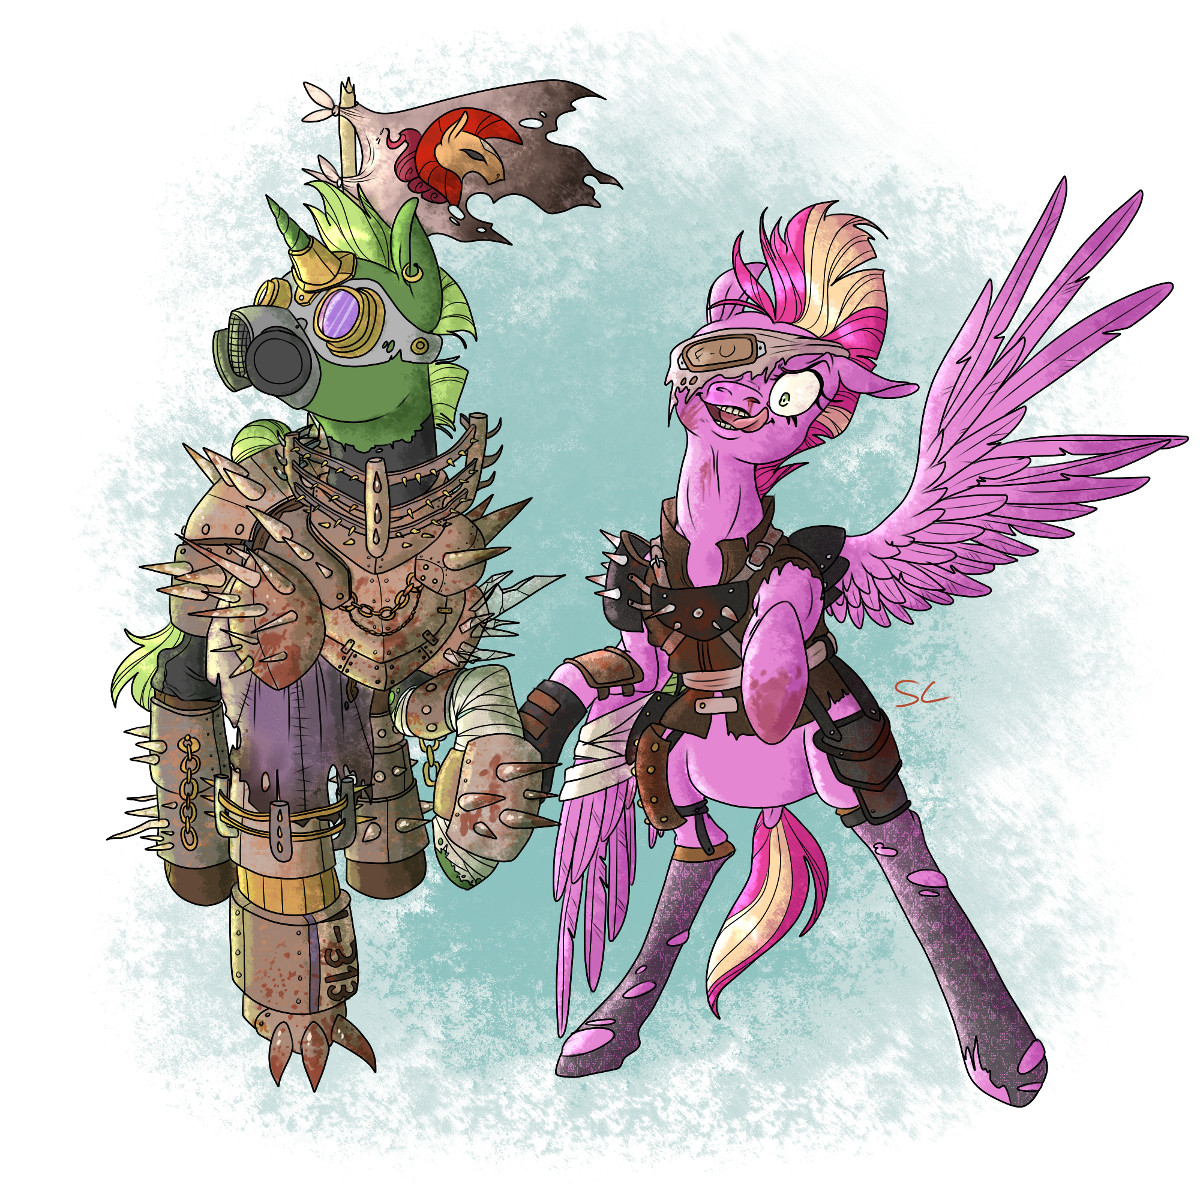
\includegraphics[width=0.6\linewidth]{ART/Enemies/raiders}
	\end{wrapfigure}

	Raiders are one of the more mix-match groups that wander the Wastes, though most common race is a pony for the sheer fact that ponies often outnumber the other races.
	
	Raiders are known for their penchant for horrid, over-the-top violent acts such as stringing corpses to ceilings, mutilating both corpses and the living alike. Reasons why raiders behave as they do are difficult to pinpoint, as some attest it to the heavy use of alcohol and drugs, while others suggest a special brain disease that turns them hostile and yet another claims desperate situation and higher susceptibility to mental illnesses. 
	
	Raiders are often violent towards both outsiders and those in their own group they view weak or inferior. Due to this, raiders are rather lackluster group who listen to one person only; themselves. Raider initiation rituals are quite savage, including severe beatings and dangerous doses of drugs. 
	A considerably strong individual can rise to the rank of a raider overboss, the de-facto leader of the group by being stronger and more menacing than the rest of the group. This will however mean that said individual will always be doomed to keep their guard up, lest they be taken down from their position by power-hungry usurpers.
	
	Though is is easy to imagine that raiders value physical strength only, there have been instances where a particularly brutal and cunning unicorns has risen in the ranks all the way to overboss-status. It could be said that on some level, raiders approve all kind of power, be it brawn, magic or high intelligence, if it can be put to good use.
	
	In combat, raiders prefer to attack head-on, trying to overwhelm their opponents with numbers, and use combat drugs such as Dash and Stampede to their advantage. Their use of drugs have left them unpredictable, but they do still have a sense of self-preservation; when things start to turn bad for them, they will attempt to flee.
	
	\clearpage

	\section*{Robobrain}
	\addcontentsline{toc}{section}{Robobrain}
	\begin{quote}
		\emph{``Somepony had the bright idea to use various brains for these robots, apparently in order to have the most advanced artificial intelligence - well, no longer artificial due the brains. A unique mix of biology and technology, these cylindrical robots on tracks perform well. As long as the brain-turned-processor hasn't malfunctioned or decayed too much in the centuries after their manufacture.''}
		
		\emph{-	Scribe Star Twinkle}
	\end{quote}
	
	\emph{\textbf{Type:} Machine}
	
	\emph{\textbf{EXP:} 200}
	
	{
		\rowcolors{1}{gray!30}{gray!10}
		\begin{tabu} to 150mm{| X[c,1] | X[c,1] | X[c,1] | X[c,1] | X[c,1] | X[c,1] | X[c,1] | X[c,1] |  X[c,3] | X[c,3]| X[c,3] | X[c,3] | X[c,3] |}
			\hline
			\multicolumn{13}{|c|}{\cellcolor{gray!50} Robobrain Statistics}                 \\ \hline
			S & P & E & C & I & A & L & \cellcolor{gray!50} & HP & DT & AP & Size & Karma   \\
			5 & 5 & 5 & 6 & 6 & 4 & 4 & \cellcolor{gray!50} & 11 & 20 & 12 & 0    & Varies* \\ \hline
		\end{tabu}
		
		\emph{*see Additional Combat Details}
	}
	
	\bigskip
	{
		\rowcolors{1}{gray!30}{gray!10}
		\begin{tabu} to 150mm{| X[c,1] | X[c,1] | X[c,1] | X[c,1] | X[c,1] | X[c,1] |}
			\hline
			\multicolumn{6}{|c|}{\cellcolor{gray!50} Skills}        \\ \hline
			Firearms & MEW & Melee & Unarmed & Diplomacy* & Barter* \\
			50       & 60  & 55    & 40      & 50         & 50      \\ \hline
		\end{tabu}
		\emph{*see Additional Combat Details}
		
	}
	
	\subsubsection*{Additional Combat Details:}
	\begin{verse}
		\textbf{Mesmerize (8 AP):} Robobrains have a mesmerizer built into them, causing their target to become Mind-Controlled. The target has to be directly in front of the robobrain for the attack to work. The target may roll INT -1 to resist the effect.
	
		\textbf{Wasteland Weaponry:} Robobrains have internal weaponry of various models, though mostly using MEWs.
	
		\textbf{*Sentience:} As a rare occurrence, Robobrains may retain their sentient minds. A sentient Robobrain has additional +2 INT, as well as access to Diplomacy and Barter. 
	
		\textbf{Coded Killer:} Even if the Robobrain was lucid enough to keep their sanity, their programming often overrides peaceful solutions. Trying to intimidate or solve matters without violence against the Robobrain always has -10 penalty.
	
		\textbf{Poison Immunity:} Due to their nature as a machine, Robobrains have immunity to poisons.
		
		\textbf{Rad Immunity:} The robobrain's metal body is immune to the effects of Radiation.
	\end{verse}
	
	\subsubsection*{Creature drops:}
	\begin{compactitem}
		\item Scrap Metal (1d4, Mechanics doubles u.)
		\item Scrap Electronics (1d4, Science doubles u.)
		\item Junk (1d8)
		\item Random Firearm or MEW (1 u.)
	\end{compactitem}
	
	
	\subsection*{Description:}
	Robobrain was a solution for the problem of creating a robot with perfect artificial intelligence - by installing a brain of a pony or other sentient being as the central processing unit, housed in a preservative gel to not decay faster than the robot's metallic exterior. 
	
	While a feat of genius, and successful in its own right, the project had some limitations - of both moral and design variety. Brains had to be extracted from living or recently deceased individuals to have minor chances of malfunction, and even then the sudden change may have proven detrimental to the now-mechanical being's mental health. And when those malfunctions occured, it proved to make the robobrains mad. No pun intended. 
	
	Robobrains roam the wastes aimlessly, seeking something to do - or patrol the areas where they were stationed as assistants and general help, working away still after all the years. Most models have been created with speakers attached, providing a way for the long-deceased owner of the brain-turned-CPU to speak his or her mind. That is, if they haven't suffered a major malfunction already. 
	
	\begin{figure}[h]
		\centering
		\includegraphics[width=0.8\linewidth]{"ART/Enemies/robobrain"}
	\end{figure}
	
	\clearpage

	\section*{Salamander}
	\addcontentsline{toc}{section}{Salamander}
	\begin{quote}
		\emph{``Shortly after they were discovered, they became a household pet and guard lizard for many ponies, until that bugger decided to grow up and eat its owner.  Needless to say, that fad died as quickly as it started. Some wager two ghoul merchants were behind the fad.''}
		
		\emph{-	Verdant Brink, hunter}
	\end{quote}
	
	\emph{\textbf{Type:} Mutated Animal}
	
	\emph{\textbf{EXP:} 150}
	
	{
		\rowcolors{1}{gray!30}{gray!10}
		\begin{tabu} to 150mm{| X[c,1] | X[c,1] | X[c,1] | X[c,1] | X[c,1] | X[c,1] | X[c,1] | X[c,1] |  X[c,3] | X[c,3]| X[c,3] | X[c,3] | X[c,3] |}
			\hline
			\multicolumn{13}{|c|}{\cellcolor{gray!50} Salamander Statistics}                  \\ \hline
			S & P & E & C & I & A & L & \cellcolor{gray!50} & HP & DT & AP & Size & Karma \\
			8 & 4 & 8 & 3 & 2 & 6 & 7 & \cellcolor{gray!50} & 16 & 20 & 12 & 1    & 0     \\ \hline
		\end{tabu}
		
		%\emph{*see Additional Combat Details}
	}
	
	\bigskip
	{
		\rowcolors{1}{gray!30}{gray!10}
		\begin{tabu} to 60mm{| X[c,1] | X[c,1] |}
			\hline
			\multicolumn{2}{|c|}{\cellcolor{gray!50} Skills} \\ \hline
			Unarmed & Sneak                          \\
			65      & 40                             \\ \hline
		\end{tabu}
		
	}

	\subsubsection*{Additional Combat Details:}
	\begin{verse}
		\textbf{Flame Spit (8 AP, 1/min):} The salamander accurately spits a ball of flame against anyone threatening it. This attack affects an area equal to Tiny Burst template, and a maximum range of 20 meters (10 hexes). Anyone caught in the area must roll END -2 or suffer  Burning status effect.
	
		\textbf{Bite (4 AP):} Salamander tries to take a bite out of its opponent, dealing 30+(2) damage. The attack also has a base 20\% chance to Cripple a limb.
	
		\textbf{Heated Scales:} The salamander's hide is its main defensive mechanism, causing burns and pain to any aspiring predator - or hunter. After every Melee or Unarmed attack (not ranged) the attacker must roll END or suffer Burning status effect.
	
		\textbf{Fire Absorber:} Salamanders are immune to damage from heat and fire, and each attack dealing fire damage heals them by 1 HP.
	
		\textbf{Cold Resistant:} Salamander's heated scales are also a way for it to regulate body heat, meaning that the creature is far more resistant to cold. They have +5 DT against cold damage.
	
		\textbf{Poison Immunity:} The high temperature that the Salamander has burns away most poisons, giving them an immunity to poison.
	
		\textbf{Rad Resistant:} Due to their mutations, Salamanders have a higher resistance to radiation, with Rad Resistance of 40.
	\end{verse}
	
	
	
	\subsubsection*{Creature Drops:}
	\begin{compactitem}
		\item Fire Resistant Hide (2 u. Survival doubles u.)
		\item Teeth (1d6, Survival doubles u.)
		\item Tail (1 u.)
		\item Junk (1d4)
	\end{compactitem}
	
	\subsection*{Description:}
	Salamanders are lizards, capable of not only withstanding flames but able to spout them. Their characteristic red or orange hide, marked with dark spots along their back easily stands out amidst the remnants of green. While still in their hatchling stage, they're nothing more than a pest, and often an adorable one, being much smaller than your average pony while only managing to spout small flares. Once they grow to adulthood, however, the cuteness dissipates - easily towering over ponies, they defend their territory fiercely, often with their trademark flame spit. And they  consider ponies to be part of their diet.
	
	Salamanders are a common pest species in more arid environments of the Equestrian Wasteland, having taken a liking to various ruins left behind by ponies. Salamanders keep their hide in check by staying warm, and best way they achieve this is by creating small fires wherever they go. They do fight over same territory with geckos, and often where there is one species, the other is nowhere to be found. It is, however, often the salamanders who come out on top if the two species duke it out.
	
	\clearpage

	\section*{Shade}
	\addcontentsline{toc}{section}{Shade}
	\begin{quote}
		\emph{``A shadow etched forever onto a surface by the irradiated necromantic force of the Megaspell. Though the pony themselves have long since perished, their shadows continue onward, given ``life'' by the necromantic components of the spell. They're drawn to other shadows, both Shades and regular living ponies' shadows, hoping to merge with something living again, but usually end up consuming and corrupting instead. Some speculate that these shadows might be changelings' shadows rather than ponies'.''}
		
		\emph{-	Star Paladin Glitter Dust}
	\end{quote}
	
	\emph{\textbf{Type:} Abomination}
	
	\emph{\textbf{EXP:} 250}
	
	{
		\rowcolors{1}{gray!30}{gray!10}
		\begin{tabu} to 150mm{| X[c,1] | X[c,1] | X[c,1] | X[c,1] | X[c,1] | X[c,1] | X[c,1] | X[c,1] |  X[c,3] | X[c,3]| X[c,3] | X[c,3] | X[c,3] |}
			\hline
			\multicolumn{13}{|c|}{\cellcolor{gray!50} Shade Statistics}              \\ \hline
			S & P & E & C & I & A & L & \cellcolor{gray!50} & HP & DT & AP & Size & Karma \\
			3 & 8 & 6 & 6 & 5 & 5 & 6 & \cellcolor{gray!50} & 5  & 5  & 12 & 0    & 0     \\ \hline
		\end{tabu}
		
		%\emph{*see Additional Combat Details}
	}
	
	\bigskip
	{
		\rowcolors{1}{gray!30}{gray!10}
		\begin{tabu} to 60mm{| X[c,1] | X[c,1] |}
			\hline
			\multicolumn{2}{|c|}{\cellcolor{gray!50} Skills} \\ \hline
			Unarmed & Sneak                          \\
			65      & 70                             \\ \hline
		\end{tabu}
		
	}
	
	\subsubsection*{Additional Combat Details:}
	\begin{verse}
		\textbf{Enfeebling Touch (6 AP):} Direct contact with Shade can cause the target to be Stunned. This attack also deals 40+(2) damage.
	
		\textbf{Corrupting Touch (8 AP):} The Shade merges with the target's shadow, giving all of the target's actions +1 AP penalty. For each full round the Shade is merged in a shadow, the target removes a HP token, ignoring DT, on the Shade's turn. Shade can still attack targets other than the one it has merged with, with the Enfeebling Touch. Bright light, such as casting Light or complete darkness forces the Shade to abandon their target's shadow. 
	
		\textbf{Unliving:} Shades pass through solid, non-magical objects like incorporeal ghosts. Due to this, conventional, non-magical weapons do not harm them. Magical weaponry like MEWs and Spirits do. They also cannot be killed per say, but if their HP is brought to a 0, they are dispersed for a day after which they reform themselves.
	
		\textbf{Painless:} Shades feel no pain, and as such, do not suffer from Pain Thresholds.
	
		\textbf{Poison Immunity:} As shades can hardly be considered alive, they are naturally immune to poisons.
	
		\textbf{Rad Immunity:} Due to the necromantic energies that sustain the shade, they are very well adapted to irradiated areas, even ground zero. They are immune to the effects of Radiation.
	\end{verse}
	
	\subsubsection*{Creature drops:}
	None
	
	\subsection*{Description:}
	A living shadow. That's what common folk tell stories about. And for the same common folk, it's a description perfect enough. A shade's a moving, seemingly instinct-following shadow of truly vile necrotic nature. But it is in all manners of science, a non living entity.
	
	Shades are - for the simplicity of words - born from the grand overdose of Radiation burning the victim's shadow, and part of it's essence by all knowledge gathered so far, permanently to the place they perished. 
	
	The terrors shades can bring upon even for the most careful of travellers, are nigh undetectable while lying in wait of even smallest of shadows, striking their prey both at the body, and at the shadow they cast. The touch of a shade feels like being burned with a frozen flame within but maybe more terrifying is the possibility of a shade taking possession of one's own shadow, and by that their whole body. And while shades are often limited to the place of their birth, the place can be anything from a small hut, to a huge mansion, a garden or a castle.
	
	\begin{figure}[h]
		\centering
		\includegraphics[width=0.7\linewidth]{"ART/Enemies/Shade"}
	\end{figure}
	
	\clearpage

	\section*{Slaver}
	\addcontentsline{toc}{section}{Slaver}
	\begin{quote}
		\emph{``While I personally detest slavery, I would rather do trade with a slaver than try to bargain a deal with a raider... A slaver is usually interested in just two things, caps or slaves. And hope it is caps they currently have on their minds, or you might find some rather heavy jewellery adorning your neck the moment you let your guard down. If it is any help, at least they want you alive and relatively healthy.''}
		
		\emph{-	Merchant Silver Bit}
	\end{quote}
	
	\emph{\textbf{Type:} Sentient}
	
	\emph{\textbf{EXP:} 150}
	
	{
		\rowcolors{1}{gray!30}{gray!10}
		\begin{tabu} to 150mm{| X[c,1] | X[c,1] | X[c,1] | X[c,1] | X[c,1] | X[c,1] | X[c,1] | X[c,1] |  X[c,3] | X[c,3]| X[c,3] | X[c,3] | X[c,3] |}
			\hline
			\multicolumn{13}{|c|}{\cellcolor{gray!50} Slaver Statistics}                       \\ \hline
			S & P & E & C & I & A & L & \cellcolor{gray!50} & HP & DT     & AP & Size & Karma \\
			6 & 6 & 5 & 7 & 6 & 5 & 6 & \cellcolor{gray!50} & 15 & Varies & 12 & 0*   & -25   \\ \hline
		\end{tabu}
		
		\emph{*Size can vary depending on species}
	}
	
	\bigskip
	{
		\rowcolors{1}{gray!30}{gray!10}
		\begin{tabu} to 150mm{| X[c,1] | X[c,1] | X[c,1] | X[c,1] | X[c,1] | X[c,1] |}
			\hline
			\multicolumn{6}{|c|}{\cellcolor{gray!50} Skills}      \\ \hline
			Firearms & MEW & Melee & Unarmed & Diplomacy & Barter \\
			60       & 60  & 40    & 40      & 60        & 70     \\ \hline
		\end{tabu}
		
	}
	
	\subsubsection*{Additional Combat Details:}
	\begin{verse}
		\textbf{Wasteland Weaponry:} Slavers can carry just about any weapon and armor imaginable, and most commonly wielding quality guns and MEWs, light armor, and occasional fancy clothes.
	
		\textbf{Greedy:} Slavers can be swayed by money, after all, that's their primary motivation. Bartering with slavers with money or bribes has a bonus of +5 on Barter.
	
		\textbf{Organized:} Slavers have hierarchy of leadership. They strike as units and groups of various sizes, usually under at least one spokesperson. Eliminating such spokesperson often leaves rest of the  group at disarray and demoralized, giving them a -5 to all skill actions.
	
		\textbf{Poison Resistant:} Slavers are most commonly ponies, zebras or griffins, thus they have their resistances reflecting this. They have Poison Resistance of 10 (20 if they are Zebras). Equipped armor can change these numbers.
	
		\textbf{Rad Resistant:} Slavers commonly have 5\% natural Radiation resistance, but most equip armor fitting to increase their tolerance against the magical fallout.
	\end{verse}
	
	\subsubsection*{Creature drops:}
	\begin{compactitem}
		\item Main Weapon (1 u.)
		\item Additional Weapon (1 u.)
		\item Armor or Clothing (1 u.)
		\item Caps (100-200 caps, LCK doubles u.)
		\item Healing item or Chems (1, LCK doubles u.)
		\item Ammo, Firearms
	\end{compactitem}
	
	\subsection*{Description:}
	Slavers aren't quite as mad as raiders, but more ruthless and greedy than mercenaries. Their main source of income and life is to rush into unsuspecting or undefended homes and settlements, take any or all ponies they can, and sell them away to some immoral wastelander who needs cheap workforce. Or something else.
	
	As such, slavers are widely despised and often not bargained with by more civilized folks. This drives these ``wasteland entrepreneurs'' to stick to their own groups and form their own camps and fortresses. They do not, however, barricade themselves in, making excursions to the wastes to keep up their lifestyle and ``might makes right'' mentality.
	
	Unlike Raiders who often act in a lackluster manner, slavers do keep a relatively tight hierarchy and organization for maximum efficiency and profit. Yet, one could say that a particularly nasty slaver is willing to sell anypony, friendships and history be damned.
	
	\begin{figure}[h]
		\centering
		\includegraphics[width=0.8\linewidth]{"ART/Enemies/slavers"}
	\end{figure}
	
	\clearpage

	\section*{Snake, Two-headed}
	\addcontentsline{toc}{section}{Snake, Two-headed}
	\begin{quote}
		\emph{``This is your garden variety viper turned huge and multiheaded, kind of like a tiny Hydra, except it doesn't have a lizard-like body. What it does have is poisonous fangs and in some cases, habit of squeezing their targets lifeless. What is worse is that all the heads are poisonous, making them more formidable than any would prefer. At least they make fantastic boots.''}
		
		\emph{-	Verdant Brink, Hunter}
	\end{quote}
	
	\emph{\textbf{Type:} Mutated Animal}
	
	\emph{\textbf{EXP:} 100}
	
	{
		\rowcolors{1}{gray!30}{gray!10}
		\begin{tabu} to 150mm{| X[c,1] | X[c,1] | X[c,1] | X[c,1] | X[c,1] | X[c,1] | X[c,1] | X[c,1] |  X[c,3] | X[c,3]| X[c,3] | X[c,3] | X[c,3] |}
			\hline
			\multicolumn{13}{|c|}{\cellcolor{gray!50} Snake Statistics}                    \\ \hline
			S & P & E & C & I & A & L & \cellcolor{gray!50} & HP & DT & AP  & Size & Karma \\
			6 & 6 & 5 & 5 & 3 & 6 & 7 & \cellcolor{gray!50} & 8  & 10 & 10* & 0    & 0     \\ \hline
		\end{tabu}
		
		\emph{*See Additional Combat Details}
	}
	
	\bigskip
	{
		\rowcolors{1}{gray!30}{gray!10}
		\begin{tabu} to 60mm{| X[c,1] | X[c,1] |}
			\hline
			\multicolumn{2}{|c|}{\cellcolor{gray!50} Skills} \\ \hline
			Unarmed & Sneak                                  \\
			60      & 70                                     \\ \hline
		\end{tabu}
		
	}
	
	\subsubsection*{Additional Combat Details:}
	\begin{verse}
		\textbf{Bite (3 AP):} The snake takes a bite out of their target, dealing 10+(3) damage.
		
		\textbf{Venomous Spit (5 AP):} Much like certain species of cobras, the two-headed snake can spit out venom from its fangs. This attack deals 15+(3) damage, and if it pierces DT, can cause the following effects, with 2x50\% chance of poisoning: 
		\begin{compactitem}
			\item On skin-contact, this venom causes a burning sensation and painful blisters, giving the target Burning Status effect. 
			\item If the venom gets to the eyes, the target suffers a penalty of -2 to PER when using eye-sight, as well as a -5 to Combat skills.
			\item Note: Snakes have either Venomous Spit or Constrict attack at their disposal
		\end{compactitem}
	
		\textbf{Constrict (5 AP):} Some snakes have evolved to wrap themselves around their target and squeezing the life out of them. For each round that the snake has constricted around a target, it deals 15+(3) damage. Once the snake lets go of the target, the target is inflicted with the Stun- Status Effect.
		\begin{compactitem}
			\item Note: Snakes have either Venomous Spit or Constrict attack at their disposal
		\end{compactitem}
	
		\textbf{*Multiple Heads:} Snakes can control their heads independently from each other, giving the creature more sources to attack with. the snake's AP is 10 + the number of heads it has.
	
		\textbf{Escape Artist:} When grappled, the snake begins to wriggle and writhe to break free, their scaly body and frantic movements easing the escape. Snakes gain a +2 to AGI and +10 to Unarmed when using Break Free -action, or when trying to Escape from the Grapple.
	
		\textbf{Poison Resistant:} Though often poisonous themselves, snakes can still fall victim to other poisons. Their poison resistance is 50\%
	
		\textbf{Rad Resistant:} Despite being a mutated creature, snakes do not have a high tolerance to Rads. Their Rad resistance is 20.
	\end{verse}
	
	\subsubsection*{Creature drops:}
	\begin{compactitem}
		\item Venom Sac (1 u.)
		\item Hide (1 u.)
		\item Teeth (6 u.)
	\end{compactitem}
	
	\subsection*{Snake, Three-headed}
	\addcontentsline{toc}{subsection}{Snake, Three-headed}
	\emph{\textbf{Type:} Mutated Animal}
	
	\emph{\textbf{EXP:} 150}
	
	{
		\rowcolors{1}{gray!30}{gray!10}
		\begin{tabu} to 150mm{| X[c,1] | X[c,1] | X[c,1] | X[c,1] | X[c,1] | X[c,1] | X[c,1] | X[c,1] |  X[c,3] | X[c,3]| X[c,3] | X[c,3] | X[c,3] |}
			\hline
			\multicolumn{13}{|c|}{\cellcolor{gray!50} Snake Statistics}                    \\ \hline
			S & P & E & C & I & A & L & \cellcolor{gray!50} & HP & DT & AP  & Size & Karma \\
			7 &	6 &	6 &	4 &	3 &	6 &	7 & \cellcolor{gray!50} & 8  & 10 & 10* & 1    & 0     \\ \hline
		\end{tabu}
		
		\emph{*See Additional Combat Details}
	}
	
	\bigskip
	{
		\rowcolors{1}{gray!30}{gray!10}
		\begin{tabu} to 60mm{| X[c,1] | X[c,1] |}
			\hline
			\multicolumn{2}{|c|}{\cellcolor{gray!50} Skills} \\ \hline
			Unarmed & Sneak                                  \\
			65      & 75                                     \\ \hline
		\end{tabu}
		
	}
	
	\subsubsection*{Additional Combat Details:}
	\begin{verse}
		\textbf{Bite (3 AP):} The snake takes a bite out of their target, dealing 15+(4) damage.
	
		\textbf{Venomous Spit (5 AP):} Much like certain species of cobras, the two-headed snake can spit out venom from its fangs. This attack deals 15+(4) damage, and if it pierces DT, can cause the following effects, with 2x50\% chance of poisoning: 
		\begin{compactitem}	
			\item On skin-contact, this venom causes a burning sensation and painful blisters, giving the target Burning Status effect. 
			
			\item If the venom gets to the eyes, the target suffers a penalty of -2 to PER when using eye-sight, as well as a -5 to Combat skills.
			
			\item Note: Snakes have either Venomous Spit or Constrict attack at their disposal
		\end{compactitem}
		\textbf{Constrict (5 AP):} Some snakes have evolved to wrap themselves around their target and squeezing the life out of them. For each round that the snake has constricted around a target, it deals 15+(4) damage. Once the snake lets go of the target, the target is inflicted with the Stun- Status Effect.
		\begin{compactitem}	
			\item Note: Snakes have either Venomous Spit or Constrict attack at their disposal
		\end{compactitem}
		
		\textbf{*Multiple Heads:} Snakes can control their heads independently from each other, giving the creature more sources to attack with. the snake's AP is 10 + the number of heads it has.
	
		\textbf{Escape Artist:} When grappled, the snake begins to wriggle and writhe to break free, their scaly body and frantic movements easing the escape. Snakes gain a +2 to AGI and +10 to Unarmed when using Break Free -action, or when trying to Escape from the Grapple.
	
		\textbf{Poison Resistant:} Though often poisonous themselves, snakes can still fall victim to other poisons. Their poison resistance is 50\%
	
		\textbf{Rad Resistant:} Despite being a mutated creature, snakes do not have a high tolerance to Rads. Their Rad resistance is 20.
	\end{verse}
	
	\subsubsection*{Creature drops:}
	\begin{compactitem}
		\item Venom Sac (2 u.)
		\item Hide (2 u.)
		\item Teeth (8 u.)
	\end{compactitem}
	
	\subsection*{Description:}
	In old days, snakes would vary between size of a hoof, and two griffons. However, small ones would often be highly venomous, while large snakes would constrict their prey to death. Sometimes the prey can be several sizes larger than the snake, yet the snake will swallow the prey whole. Known to be loners, snakes would only be seen in groups during mating seasons, and as mad collector's pets.
	
	As Wasteland was born, magical residue would transform many snakes completely twisting the belief only small snakes are venomous, as snakes would be commonly the size of an average pony. But what truly remarkable happened, was the splitting; snakes would become twin - or even tri-headed, multiplying the killing force against the fresh prey of the Wastes.
	
	\clearpage

	\section*{Spider}
	\addcontentsline{toc}{section}{Spider}
	\begin{quote}
		\emph{``Professor Hottentotta was quite interested in the effects of balefire Radiation on the common spider. It seems that depending on their genes, different effects happen. Some grew in size into truly terrifying sizes, while some developed radioactive isotopes in their venom. Truly magnificent!''}
	
		\emph{-	Acacia Honey, entomologist}
	\end{quote}
	
	\emph{\textbf{Type:} Mutated Insect}
	
	\emph{\textbf{EXP:} 50}
	
	{
		\rowcolors{1}{gray!30}{gray!10}
		\begin{tabu} to 150mm{| X[c,1] | X[c,1] | X[c,1] | X[c,1] | X[c,1] | X[c,1] | X[c,1] | X[c,1] |  X[c,3] | X[c,3]| X[c,3] | X[c,3] | X[c,3] |}
			\hline
			\multicolumn{13}{|c|}{\cellcolor{gray!50} Spider Statistics}                   \\ \hline
			S & P & E & C & I & A & L & \cellcolor{gray!50} & HP & DT & AP & Size & Karma \\
			4 & 8 & 5 & 4 & 3 & 7 & 5 & \cellcolor{gray!50} & 7  & 5  & 13 & -1   & 0     \\ \hline
		\end{tabu}
		
		%\emph{*See Additional Combat Details}
	}
	
	\bigskip
	{
		\rowcolors{1}{gray!30}{gray!10}
		\begin{tabu} to 80mm{| X[c,1] | X[c,1] |}
			\hline
			\multicolumn{2}{|c|}{\cellcolor{gray!50} Skills} \\ \hline
			Unarmed & Sneak                                  \\
			55      & 55                                     \\ \hline
		\end{tabu}
		
	}
	
	\subsubsection*{Additional Combat Details:}
	\begin{verse}
		\textbf{Web (5 AP):} The spider entangles its target in a flung webbing, slowing them down. The target suffers a +1 AP to Movement actions.

		\textbf{Bite (4 AP):} The spider's bite is dangerous as the wounds often begin to bleed. This attack deals 20+(2) damage, and can cause Bleeding- Status effect.
	
		\textbf{Wild Dance (5 AP, 1/min):} The spiders are often colored with bright warning colors in a myriad of patterns. They can make an interpretive dance to cause a Minor Distraction.
	
		\textbf{Balanced:} Due to having 8 legs, spiders have high balance. Spiders receive +20 to resist Trip, and they ignore up to 4 crippled legs before debilitations.
	
		\textbf{Quick Runner:} Spiders, despite their size, move at a terrifying speed, giving them +2 to their Initiative rolls.
	
		\textbf{Woodlands Stride:} Spiders are capable of crawling on many surfaces which other species struggle with, thus ignoring the +1 AP cost of Difficult Terrain.

		\textbf{Poison Resistant:} Spiders are often tolerant against a myriad of poisons, and with their mutation even insecticides have trouble taking them down permanently. Their poison resistance is 70.
	
		\textbf{Rad Resistant:} The magical mutations have given spiders slight boost on their Rad resistance, but not by a substantial amount. Their Rad resistance is 30.
	\end{verse}
	
	\subsubsection*{Creature drops:}
	\begin{compactitem}
		\item Spider Legs (8 u.)
		\item Mandibles (2 u.)
		\item Poison Gland (1 u.)
	\end{compactitem}
	
	\subsection*{Spider, Giant}
	\addcontentsline{toc}{subsection}{Spider, Giant}
		
	\emph{\textbf{Type:} Mutated Insect}
	
	\emph{\textbf{EXP:} 100}
	
	{
		\rowcolors{1}{gray!30}{gray!10}
		\begin{tabu} to 150mm{| X[c,1] | X[c,1] | X[c,1] | X[c,1] | X[c,1] | X[c,1] | X[c,1] | X[c,1] |  X[c,3] | X[c,3]| X[c,3] | X[c,3] | X[c,3] |}
			\hline
			\multicolumn{13}{|c|}{\cellcolor{gray!50} Spider Statistics}                  \\ \hline
			S & P & E & C & I & A & L & \cellcolor{gray!50} & HP & DT & AP & Size & Karma \\
			6 & 8 & 5 & 4 & 3 & 7 & 5 & \cellcolor{gray!50} & 11 & 30 & 13 & 1    & 0     \\ \hline
		\end{tabu}
		
		%\emph{*See Additional Combat Details}
	}
	
	\bigskip
	{
		\rowcolors{1}{gray!30}{gray!10}
		\begin{tabu} to 60mm{| X[c,1] | X[c,1] |}
			\hline
			\multicolumn{2}{|c|}{\cellcolor{gray!50} Skills} \\ \hline
			Unarmed & Sneak                                  \\
			70      & 45                                     \\ \hline
		\end{tabu}
		
	}

	\subsubsection*{Additional Combat Details:}
	\begin{verse}
		\textbf{Web (5 AP):} The spider entangles its target in a flung webbing, slowing them down. The target suffers a +1 AP to Movement actions.
		
		\textbf{Bite (4 AP):} The spider's bite is dangerous as the wounds often begin to bleed. This attack deals 40+(2) damage, and can cause Bleeding- Status effect.
		
		\textbf{Wild Dance (5 AP, 1/min):} The spiders are often colored with bright warning colors in a myriad of patterns. They can make an interpretive dance to cause a Medium Distraction.
		
		\textbf{Balanced:} Due to having 8 legs, spiders have high balance. Spiders receive +20 to resist Trip, and they ignore up to 4 crippled legs before debilitations.
		
		\textbf{Quick Runner:} Spiders, despite their size, move at a terrifying speed, giving them +2 to their Initiative rolls.
		
		\textbf{Woodlands Stride:} Spiders are capable of crawling on many surfaces which other species struggle with, thus ignoring the +1 AP cost of Difficult Terrain.
		
		\textbf{Firm grip:} Giant spiders have their Grapple Actions cost -1 AP less, and their STR is considered +1 higher when Grappling.
		
		\textbf{Poison Resistant:} Spiders are often tolerant against a myriad of poisons, and with their mutation even insecticides have trouble taking them down permanently. Their poison resistance is 70.
		
		\textbf{Rad Resistant:} The magical mutations have given spiders slight boost on their Rad resistance, but not by a substantial amount. Their Rad resistance is 30.
	\end{verse}
	
	\subsubsection*{Creature drops:}
	\begin{compactitem}
		\item Spider Legs (8 u.)
		\item Mandibles (2 u.)
		\item Poison Gland (1 u.)
	\end{compactitem}

	\subsection*{Description:}
	Spiders haven't changed much since the bombs fell - their most striking change being the large size they've grown to. 
	
	Depending on the spider, they may produce a web in shady corners or between two standing posts, burrow underground and stalk for any passing pray, or fill a large cavity in ruins with webs to call it home. Whatever the case, they're always hunting for meat. And ponies aren't an exception on their menu.
	
	The magical radiation hasn't exactly calmed down these creatures either; they tend to attack any suitable prey, should they be hungry or feeling threatened. However, much like any animal, they're smart enough to flee when things get dicey for them.
	
	Spiders are often loners by nature, with the exception of a female with an egg sac or mating season. And for the male spider, that can end in death as well.
	
	\clearpage

	\section*{Spider-Bot}
	\addcontentsline{toc}{section}{Spider-Bot}
	\begin{quote}
		\emph{``These small, eight-legged mechanical creatures stick to the ruins where their original owners placed them. These little rascals behave like violent animals, as they will pounce on anypony daring enough to explore the rubble they call home. I bet they were used as a defensive mechanism before the War. Thankfully, instead of lethal poison they use sedatives.''}
	
		\emph{-	Scribe Star Twinkle}
	\end{quote}
	
	\emph{\textbf{Type:} Machine}
	
	\emph{\textbf{EXP:} 100}
	
	{
		\rowcolors{1}{gray!30}{gray!10}
		\begin{tabu} to 150mm{| X[c,1] | X[c,1] | X[c,1] | X[c,1] | X[c,1] | X[c,1] | X[c,1] | X[c,1] |  X[c,3] | X[c,3]| X[c,3] | X[c,3] | X[c,3] |}
			\hline
			\multicolumn{13}{|c|}{\cellcolor{gray!50} Spider-Bot Statistics}                  \\ \hline
			S & P & E & C & I & A & L & \cellcolor{gray!50} & HP & DT & AP & Size & Karma \\
			5 & 6 & 7 & 4 & 4 & 5 & 3 & \cellcolor{gray!50} & 5  & 15 & 12 & -2   & 0     \\ \hline
		\end{tabu}
		
		%\emph{*See Additional Combat Details}
	}
	
	\bigskip
	{
		\rowcolors{1}{gray!30}{gray!10}
		\begin{tabu} to 120mm{| X[c,1] | X[c,1] | X[c,1] | X[c,1] |}
			\hline
			\multicolumn{4}{|c|}{\cellcolor{gray!50} Skills} \\ \hline
			MEW & Firearms & Unarmed & Sneak                 \\
			35  & 45       & 40      & 50                    \\ \hline
		\end{tabu}
		
	}
	
	\subsubsection*{Additional Combat Details:}
	\begin{verse}
		\textbf{Sedative Shot (8 AP, 1/min):} The Spiderbot uses the injector located on its ``mouth'', shooting a sedative dart at its target (Firearms, range 10/20/40). This attack deals 10+(4) damage and may cause the target to become sedated, causing the target to suffer a +1 AP to all actions.
		
		\textbf{Spark (5 AP):} The Spider-bot attaches itself on the target's body with the small hooks it has on its eight feet and gives them a electric shock. This attack (Unarmed) deals 10+(4) damage, and can stun the target on Critical Hit.
	
		\textbf{Laser Beam (4 AP):} Spider-bots are outfitted with a Magical Energy Pistol's mechanisms inside their robotic body and deal damage accordingly.
	
		\textbf{Painless:} As a machine, Spider-Bot has no Pain Thresholds.
	
		\textbf{Poison Immunity:} As a machine, Spider-Bot is immune to toxins.
		
		\textbf{Rad Immunity:} Due to not being alive, radiation has no effect on Spider-Bots.
	\end{verse}
	
	\subsubsection*{Creature drops:}
	\begin{compactitem}
		\item Scrap Metal (1d4 u, Mechanics doubles u.)
		\item Scrap Electronics (1d4 u, Science doubles u.)
		\item Ammo - Gem Pack
		\item Junk (1d4)
	\end{compactitem}
	
	\subsection*{Description:}
	Spider-Bots resemble normal spiders a lot - they have eight mechanical legs for stability, and various sensors on the center part to detect movement and life. Over the years, the number of legs may have dropped by one or two, though that won't hinder their movement.
	
	Spider-Bots were created as a cheap, mobile yet effective defense mechanism for various commercial uses. Mimicking their more insect cousins, Spider-Bots carry around an arsenal of sedatives to utilize on ``trespassers'', as well as shocking ability and ranged magical attack for the more troublesome ``hoodlums''. 
	
	Spider-Bots are programmed as purely defensive, and thus do not roam the wastes at all. Instead, they stay in and around the very building they were assigned to, protecting it from any danger, be it a mutated animal or scavenger.
	
	\clearpage

	\section*{Spore Carrier}
	\addcontentsline{toc}{section}{Spore Carrier}
	\begin{quote}
		\emph{``These accursed creatures are a plague onto the world; former ponies taken over by a violent, transformative pollen, changing them into mindless, if strangely pretty, flowering husks. Despite their vegetative looks they're lethal, flowers or not, either infecting you or just outright killing you as you walk past them unaware, as they camouflage into vegetation perfectly.''}
		
		\emph{-	Doc Holly}
	\end{quote}
	
	\emph{\textbf{Type:} Abomination/Mutated Plant}
	
	\emph{\textbf{EXP:} 150}
	
	{
		\rowcolors{1}{gray!30}{gray!10}
		\begin{tabu} to 150mm{| X[c,1] | X[c,1] | X[c,1] | X[c,1] | X[c,1] | X[c,1] | X[c,1] | X[c,1] |  X[c,3] | X[c,3]| X[c,3] | X[c,3] | X[c,3] |}
			\hline
			\multicolumn{13}{|c|}{\cellcolor{gray!50} Spore Carrier Statistics}                  \\ \hline
			S & P & E & C & I & A & L & \cellcolor{gray!50} & HP & DT & AP & Size & Karma \\
			5 &	4 &	7 &	4 &	6 &	5 &	5 & \cellcolor{gray!50} & 5  & 15 & 12 & -2   & 0     \\ \hline
		\end{tabu}
		
		%\emph{*See Additional Combat Details}
	}
	
	\bigskip
	{
		\rowcolors{1}{gray!30}{gray!10}
		\begin{tabu} to 80mm{| X[c,1] | X[c,1] | X[c,1] |}
			\hline
			\multicolumn{3}{|c|}{\cellcolor{gray!50} Skills} \\ \hline
			Melee & Unarmed & Sneak                          \\
			60    & 55      & 40                             \\ \hline
		\end{tabu}
		
	}

	\subsubsection*{Additional Combat Details:}
	\begin{verse}
		\textbf{Slasher (7 AP):} Spore Carriers have long claw-like spikes on their feet. They can use these claws to slash at targets. This attack deals 30+(2) damage and causes Bleeding -Status Effect. This status effect doesn't refresh from multiple hits. 
		
		\textbf{Poison Barb (4 AP):} Spore Carriers fire the barbs from their body at their foes (Melee, range 10/20/40), dealing 25+(2) damage. If this attack's damage overcomes DT, it has a 2 x 40\% chance to cause a hallucination on its target for 3 rounds. If the target is poisoned, they will see double and have to roll LCK to see if they manage to hit their target when attacking.
	
		\textbf{Self-destruct:} Upon reaching 0 HP, Spore Carrier explodes with a Small Burst template centered on itself. Deals 20 + (2) damage, and can infect all who are exposed to it by breathing its spores. If the target is infected, they suffer a AGI -1 and END -1 until the spores have been removed from their body.
	
		\textbf{Camouflage:} Spore carriers have double their skill value to Sneak when hidden in vegetation. 
	
		\textbf{Poison Immunity:} The spore carriers have a full immunity to poisons due to their questionable status as alive.
	
		\textbf{Rad Immunity:} Due to Spore carriers being deceased ponies animated by a plant, they do not suffer from Radiation.
	\end{verse}
	
	\subsubsection*{Creature drops:}
	\begin{compactitem}
		\item Abomination flesh piece (1d2 u, Survival doubles u.)
		\item Spore Carrier Thorn (Thorn, 1d4, Survival doubles u.)
		\item Green Herbs (1d4 u.)
		\item Junk (1d4)
	\end{compactitem}
	
	\subsection*{Description:}
	One of the more freakish mutations the Wastes has to offer, the Spore carrier is a pony overtaken by a transformative pollen. Though the pony itself is long dead, the flower infested corpse shambles around with some strange semblance of pony behavior. Once the Spore carrier itself dies - through age or wasteland weaponry - it may sprout a new Spore Plant to continue the cycle.
	
	Spore carriers, much like ponies, are social creatures that form tight groups. There is usually a stronger alpha to lead a herd of spore carriers, sometimes called ``Spore Carrier Princess''. Due to this herd-mentality, they tend to attack in groups as well.
	
	Spore carriers are ambush-predators, hiding in vegetation until the victim has walked close enough for a quick surprise attack. When Spore carriers attack, they use both their long claw-like spikes and poisonous barbs to render the victim unconscious. The Spore carrier will then release the same transformative pollen on the victim, who will, if left untreated, turn into a Spore carrier themselves. 
	
	Generally, this transformation takes few weeks, with first symptoms showing up within a few days. The symptoms include shortness of breath, dizziness, orange spots appear on the body and finally, the victim's body starts to gain bark-like properties, before death takes them. 
	
	Thankfully, there is a cure for the affliction; a potion made of the Spore plant's sap and few Green herbs boiled in water takes care of the pollen when digested for every day about a week. 
	
	\clearpage

	\section*{Spore Plant}
	\addcontentsline{toc}{section}{Spore Plant}
	\begin{quote}
		\emph{``Spore Plant is the sole reason we have Spore Carriers. This foolish experiment gone horribly wrong has caused untold damages to various settlements. This deliberately mutated swamp plant now infects others with an infectious pollen that will eventually turn the poor victim into a Spore Carrier, or kill them. If you can keep from inhaling the spores, you're relatively safe.''}
		
		\emph{-	Doc Holly}
	\end{quote}
	
	\emph{\textbf{Type:} Mutated Plant}
	
	\emph{\textbf{EXP:} 150}
	
	{
		\rowcolors{1}{gray!30}{gray!10}
		\begin{tabu} to 150mm{| X[c,1] | X[c,1] | X[c,1] | X[c,1] | X[c,1] | X[c,1] | X[c,1] | X[c,1] |  X[c,3] | X[c,3]| X[c,3] | X[c,3] | X[c,3] |}
			\hline
			\multicolumn{13}{|c|}{\cellcolor{gray!50} Spore Plant Statistics}             \\ \hline
			S & P & E & C & I & A & L & \cellcolor{gray!50} & HP & DT & AP & Size & Karma \\
			4 & 6 & 7 & 2 & 1 & 4 & 6 & \cellcolor{gray!50} & 6  & 5  & 12 & -1   & 0     \\ \hline
		\end{tabu}
		
		%\emph{*See Additional Combat Details}
	}
	
	\bigskip
	{
		\rowcolors{1}{gray!30}{gray!10}
		\begin{tabu} to 80mm{| X[c,1] | X[c,1] | X[c,1] |}
			\hline
			\multicolumn{3}{|c|}{\cellcolor{gray!50} Skills} \\ \hline
			Melee & Unarmed & Sneak                          \\
			60    & 60      & 20                             \\ \hline
		\end{tabu}
		
	}
	
	\subsubsection*{Additional Combat Details:}
	\begin{verse}
		\textbf{Poison Barb (4 AP):} Spore plants fire the barbs from their body at their foes (Melee, range 20/40/80), dealing 30+(2) damage. If this attack's damage overcomes DT, it has a 2 x 40\% chance to poison the target and cause them to become aggressive. If the target is poisoned, they're inflicted with Enraged- status effect.
	
		\textbf{Pollen Cloud (8 AP, 1/min):} The Spore plant releases its spores should a target venture adjacent to it. However, it takes some time for the pollen to gather inside the plant. This attack has 2 x 60\% chance of poisoning their target with the spores. If a target has been infected, they suffer from AGI -1 and END -1 until the spores have been removed.
	
		\textbf{Stalk Sweep (6 AP):} The spore plant is more hardy than it lets on. It uses its long stalk to knock ponies off their hooves, almost like a flail. This attack deals 20 + (3) damage and can knock opponents prone.
	
		\textbf{Rad Healing (8 AP, 1/min):} The spore plant may choose to discard 2 Rad Tokens, and replenish an equal amount of HP Tokens and/or Crippled Conditions, if any are present.
	
		\textbf{Immobile:} Spore plants are rooted in place, so they have no movement speeds.
	
		\textbf{Fire Resistant:} Spore plants, due to their genetic modifications, are more hardy to fire. This gives them +2 to END to resist Burning- status effect.
	
		\textbf{Poison Immunity:} The I.M.P experimentation made to the swamp flower has resulted in the resulting Spore plant being immune to poisons.
	\end{verse}
	
	\subsubsection*{Creature drops:}
	\begin{compactitem}
		\item Green Herbs (1d4 u. Survival doubles u.)
		\item Red Herbs (1d4 u. Survival doubles u.)
		\item Blue Herbs  1d2 u, Survival doubles u.)
		\item Spore Plant Sap (1d6 vials, Survival -20 doubles u.)
	\end{compactitem}
	
	\subsection*{Description:}
	A result of a biological experiment gone horribly wrong after - or before - the Great War, the Spore Plant has become a nuisance in the Wasteland. Its method of multiplying relies on its spores getting inhaled by a passing being, who then slowly turns into a Spore Carrier. The Spore Carriers act also as a defending horde against anyone who dares too close to the Spore Plant. It is common to find one with the other nearby.
	
	Spore plants are rooted in place, thus they cannot pursue. However, they can use toxic barbs to shoot at far-away targets, which compels the poisoned target to become enraged. This is all in purpose of luring the victim closer for eventual pollination.
	
	These swamp plants are quite unique with how well they fare with radiation, as they are actually healed by it. Thus the Spore Plants thrive in damp swamps contaminated by fallout, and may occasionally be found in slightly flooded buildings.
	
	\clearpage

	\section*{Sprite Bot}
	\addcontentsline{toc}{section}{Sprite Bot}
	\begin{quote}
		\emph{``Unlike their biological cousins, the floating Sprite Bots aren't out there to eat everything out of existence. Quite the opposite - they are extremely useful robots. They're used for a myriad of things, like moving radio broadcasters, courier tasks and personal defense to list a few. Frankly, I'd construct one for myself in a heartbeat if I had all the computing bits!''}
		
		\emph{-	Scribe Star Twinkle}
	\end{quote}
	
	\emph{\textbf{Type:} Machine}
	
	\emph{\textbf{EXP:} 50}
	
	{
		\rowcolors{1}{gray!30}{gray!10}
		\begin{tabu} to 150mm{| X[c,1] | X[c,1] | X[c,1] | X[c,1] | X[c,1] | X[c,1] | X[c,1] | X[c,1] |  X[c,3] | X[c,3]| X[c,3] | X[c,3] | X[c,3] |}
			\hline
			\multicolumn{13}{|c|}{\cellcolor{gray!50} Sprite Bot Statistics}              \\ \hline
			S & P & E & C & I & A & L & \cellcolor{gray!50} & HP & DT & AP & Size & Karma \\
			5 & 7 & 5 & 6 & 5 & 5 & 4 & \cellcolor{gray!50} & 7  & 15 & 12 & -2   & 0     \\ \hline
		\end{tabu}
		
		%\emph{*See Additional Combat Details}
	}
	
	\bigskip
	{
		\rowcolors{1}{gray!30}{gray!10}
		\begin{tabu} to 60mm{| X[c,1] | X[c,1] |}
			\hline
			\multicolumn{2}{|c|}{\cellcolor{gray!50} Skills} \\ \hline
			MEW & Sneak                                      \\
			60  & 60                                         \\ \hline
		\end{tabu}
		
	}
	
	\subsubsection*{Additional Combat Details:}
	\begin{verse}
		\textbf{Plasma Pistol (4 AP):} Equipped for combat in longer ranges, Sprite bots have a built-in plasma pistol in their robotic body. This attack deals 20 + (1) with DT reduction of 5 and ranges of 20/40/80.
	
		\textbf{Radio Jingle (6 AP):} Sprite bots can use their internal radio-system to distract their enemies. By suddenly turning on their radio broadcast on whatever channel it happens to be in, they can cause all targets in a Medium Burst template to be Distracted.
	
		\textbf{Courier (6 AP):} Due to their programming allowing them to be used as couriers, they can sometimes put this into use in the battlefield. Sprite Bots can attempt to shoot at the enemy's weapon to disarm them, ignoring -10 penalties to the Called shot in question. If the Sprite bot successfully disarms a target, they might take the item and start to carry it further away from the target. However, this action will give the target an Attack of Opportunity.
	
		\textbf{Alert Fanfare:} Sprite bots play a catchy little jingle when they spot an enemy, alerting nearby creatures to a threat, giving their allies +1 to PER to spot sneaking enemies.
	
		\textbf{Hovering:} Sprite bots hover in the air, with a movement speed of 1 AP for 2 meters (1 Hex).
	
		\textbf{Painless:} As a machine, Sprite bot has no Pain Thresholds.
	
		\textbf{Poison Immunity:} As a machine, Sprite bot is immune to toxins.
	
		\textbf{Rad Immunity:} Due to not being alive, radiation has no effect on Sprite bots.
	\end{verse}
	
	\subsubsection*{Creature drops:}
	\begin{compactitem}
		\item Scrap Metal (1d4 u, Mechanics doubles u.)
		\item Scrap Electronics (1d4 u, Science doubles u.)
		\item Plasma Pistol (1 u.)
		\item Ammo - MFC
		\item Junk (1d4)
	\end{compactitem}
	
	\subsection*{Description}
	The Sprite-Bots are basically hovering little balls of metal, closely resembling the unmutated parasprite in exterior view. Their exact original use is unknown, but all models are equipped with a speaker, microphone and radio antenna, allowing for listening and sending messages on radio waves, as well as some sort of self-defence weapon, usually small-caliber firearm or magical weaponry. These features make the Sprite-Bot a great companion for those with knowledge on robotics - that is, if they find one that isn't either hostile or already in use by some wastelander broadcasting annoying music.
	
	Because Sprite-Bots do not usually have a defense protocol assigned to a specific building, it is common to find a Sprite-Bot wandering about in the Wastes. Due to at least seeming to be a civilian contraption and one never meant for active combat, Sprite-Bots are rather easy to hack and gain access to, when compared to a nigh-invulnerable Ultra-Sentinel.
	
	\begin{figure}[h]
		\centering
		\includegraphics[width=0.6\linewidth]{"ART/Enemies/spritebot"}
	\end{figure}
	
	\clearpage

	\section*{Steel Ranger}
	\addcontentsline{toc}{section}{Steel Ranger}
	\begin{quote}
		\emph{``You don't get trouble from Steel Rangers as long as you keep your head low and your wares low-tech. Unless the customer has their Power Armor-helmeted head too far up their arses and they see fit to bully you for kicks. Thankfully, I hear a sensible few decided to leave the faction and help the common pony instead of robbing liberating anypony with anything nigh better than a peashooter for a weapon.''}    
		 
		\emph{-	Merchant Silver Bit }
	\end{quote}
	
	\emph{\textbf{Type:} Sentient}
	
	\emph{\textbf{EXP:} 500}
	
	{
		\rowcolors{1}{gray!30}{gray!10}
		\begin{tabu} to 150mm{| X[c,1] | X[c,1] | X[c,1] | X[c,1] | X[c,1] | X[c,1] | X[c,1] | X[c,1] |  X[c,3] | X[c,3]| X[c,3] | X[c,3] | X[c,3] |}
			\hline
			\multicolumn{13}{|c|}{\cellcolor{gray!50} Steel Ranger Statistics}             \\ \hline
			S & P & E & C & I & A & L & \cellcolor{gray!50} & HP & DT & AP & Size & Karma  \\
			7 & 6 & 8 & 5 & 6 & 4 & 7 & \cellcolor{gray!50} & 18 & 50 & 12 & 0    & Varies \\ \hline
		\end{tabu}
		
		%\emph{*See Additional Combat Details}
	}
	
	\bigskip
	{
		\rowcolors{1}{gray!30}{gray!10}
		\begin{tabu} to 150mm{| X[c,1] | X[c,1] | X[c,1] | X[c,1] | X[c,1] | X[c,1] |}
			\hline
			\multicolumn{6}{|c|}{\cellcolor{gray!50} Skills}               \\ \hline
			MEW & Explosives & Science & Mechanics & Barter & Intimidation \\
			70  & 50         & 70      & 60        & 50     & 70           \\ \hline
		\end{tabu}
		
	}
	
	\subsubsection*{Additional Combat Details:}
	\begin{verse}
		\textbf{Wasteland Weaponry:} As sentient creatures, Steel Rangers sport a myriad of weaponry, and take great liking in high-end magical weapons. Their patrols wear Power Armor exclusively, but Steel Stranger Scribes can be seen wearing lighter armor.
	
		\textbf{Greedy:} Steel Rangers can be swayed by technology, which is often their primary goal. Bartering with Steel Rangers with rare technology, has a bonus of +5 on Barter.
	
		\textbf{Organized:} Steel Rangers have hierarchy of full military leadership. They strike as units and groups of various sizes, usually under at least one commander. Eliminating such commander often leaves rest of the  group at disarray and demoralized, giving them a -5 to all skill actions.
	
		\textbf{Abomination Hunter:} Due to their high-caliber weaponry and armor, most Steel Rangers are well-equipped to fight even the most horrid things the Wasteland has to offer. They gain a +10 to Combat skills when targeting Abominations, including sane Ghouls.
	
		\textbf{Poison Resistant:} As Steel Rangers are exclusively ponies, their resistances reflect this. They have Poison Resistance of 10. Equipped armor can change these numbers.
	
		\textbf{Rad Resistant:} Steel Rangers commonly have 5\% natural Radiation resistance, but most equip armor fitting to increase their tolerance against the magical fallout.
	\end{verse}
	
	\subsubsection*{Creature drops:}
	\begin{compactitem}
		\item Main Weapon (1 u.)
		\item Additional Weapon (1 u.)
		\item Power Armor (1 u., cannot be used without \emph{Power Armor training})
		\item Skill Book (1 u. LCK -20 to obtain)
		\item Junk (1d6 u.)
	\end{compactitem}
	
	\subsection*{Description:}
	The Steel Rangers are a technologically-advanced faction of the remnants of Equestrian military and two Ministries, composed of Earth Ponies and Unicorns. One can easily identify a Steel Ranger from the distinctive form of high-tech full-body armor, noted as Power Armor.
	
	While originally the Steel Rangers' oath was to the protection of Equestrian populace, their goals have shifted to the acquisition and research of advanced pre-War technology in the hopes they may duplicate it. This drive for technology adds to their immersive arsenal of weaponry - often making encounters with them highly risky if one has something the Rangers are after.
	
	The Rangers' command structure is hierarchical and extremely rigid. A commanding officer can only issue commands to their direct subordinate, and a commanding officer's orders should not be questioned. At the top of every chapter of Steel Rangers sits an Elder, whose words are final.
	
	\clearpage

	\section*{Star-Spawn}
	\addcontentsline{toc}{section}{Star-Spawn}
	\begin{quote}
		\emph{``Star-Spawns... I think zebras think they're some kind of horrid demon, and most ponies would agree, due to how destructive they can get even on accident. Though their body is composed of stars and they're nearly invisible, they have some real power behind their seemingly ethereal appearance. Don't go against one unless you know what you're doing...''}
		
		\emph{-	Verdant Brink, Hunter}
	\end{quote}
	
	\emph{\textbf{Type:} Non-Mutated Animal}
	
	\emph{\textbf{EXP:} 1500}
	
	{
		\rowcolors{1}{gray!30}{gray!10}
		\begin{tabu} to 150mm{| X[c,1] | X[c,1] | X[c,1] | X[c,1] | X[c,1] | X[c,1] | X[c,1] | X[c,1] |  X[c,3] | X[c,3]| X[c,3] | X[c,3] | X[c,3] |}
			\hline
			\multicolumn{13}{|c|}{\cellcolor{gray!50} Star-Spawn Statistics}              \\ \hline
			S  & P & E  & C & I & A & L & \cellcolor{gray!50} & HP & DT & AP & Size & Karma \\
			12 & 6 & 10 & 3 & 5 & 6 & 8 & \cellcolor{gray!50} & 22 & 50 & 13 & 4    & 0     \\ \hline
		\end{tabu}
		
		%\emph{*See Additional Combat Details}
	}
	
	\bigskip
	{
		\rowcolors{1}{gray!30}{gray!10}
		\begin{tabu} to 80mm{| X[c,1] | X[c,1] | X[c,1] |}
			\hline
			\multicolumn{3}{|c|}{\cellcolor{gray!50} Skills} \\ \hline
			Melee & Unarmed & Sneak                          \\
			75    & 60      & 80                             \\ \hline
		\end{tabu}
		
	}
	
	\subsubsection*{Additional Combat Details:}
	\begin{verse}
		\textbf{Roar (8 AP):} Star-Spawn roar sends out a shockwave strong enough to send opponents stumbling back, knocking them prone in a Huge Burst template. Targets of this attack may try to remain upright with a -2 STR roll.
	
		\textbf{Slow Stomp (8 AP):} Star-Spawns can cause terrible injury with a mere step. A Star-Spawn's Slow Stomp deals 60+(4) damage on a Small Burst template. Any target underneath may roll AGI -1 to get out of the way in time.
	
		\textbf{Tremor (12 AP):} Star-Spawn crashes all its gargantuan size to the ground, often simply by sitting down. This action takes 3 turns, 1 turn to sit down, and 2 turns to complete the trembles. Every grounded character within 100 meters (50 hex) must succeed a STR or AGI roll with -3 penalty or be knocked prone, on both turns of the trembles. Any character within a Large Burst Template will take 50 + (2) damage, and additional (5) if knocked prone due to grumbling ground practically crushing its victim.
	
		\textbf{Invisible Limbs:} Star-Spawn limbs are nearly invisible, raising the penalty of Called shots to its limbs by 20.
	
		\textbf{Destroyer:} Star-Spawn can and often do remove covers and obstacles from the battlefield with a single strike of paw.
	
		\textbf{Poison Resistant:} Star-Spawns have a very high tolerance for most things, considering their nature. Their Poison resistance is 90.
	
		\textbf{Rad Immunity:} Star-Spawn have a natural immunity to magical radiation, and thus they have not mutated.
	\end{verse} 
	
	\subsubsection*{Creature drops:}
	None
	
	\subsection*{Description:}
	Star-Spawn is one of the most threatening creatures the Equestrian Wasteland has ever seen. Often doing terrible damage to its surroundings simply by walking through a settlement or by sitting down to take a nap.
	
	Gargantuan in size, these star-patterned bears hail from the pre-war Equestrian Ursa Major, a mythological bear with a see-through body of stars. In fact, the changes to this creature are nearly non-existing; aside from the slight increase to size and more see-through body, little has changed in the Star-Spawn. These creatures are quite difficult to take down due to their nearly invisible body, and their size and strength.
	
	Linked to many zebra myths, these bears are the ultimate ill omen for a zebra tribe, as their star-patterns are seen as something beyond evil incarnate, feared by many. Thankfully, star-spawn territories can easily span half a country, meaning that it is quite rare to run into one.
	
	Star-Spawn are solitary creatures, but their females are noticeably caring mothers, caring for their offspring well beyond their infant years. The cub is a curious thing, eventually beginning to wander off from their nest and usually end up in some poor settlement when taking a stroll.
	
	\clearpage

	\section*{Tankbug}
	\addcontentsline{toc}{section}{Tankbug}
	\begin{quote}
		\emph{``I saw, no kidding, a millipede the size of a bus, happily crawling forward. Truly, I am happy I am here in the research labs, able to watch it from afar. It seems quite docile, though I did see it trample a couple of... I don't know how to call them? Survivors I guess? That tried to get on its path. The resulting remains were a lot like a tank had ran them over. I think I'll call this one a Tankbug.''}

		\emph{-	Acacia Honey, Entomologist}
	\end{quote}
	
	\emph{\textbf{Type:} Mutated Insect}
	
	\emph{\textbf{EXP:} 250}
	
	{
		\rowcolors{1}{gray!30}{gray!10}
		\begin{tabu} to 150mm{| X[c,1] | X[c,1] | X[c,1] | X[c,1] | X[c,1] | X[c,1] | X[c,1] | X[c,1] |  X[c,3] | X[c,3]| X[c,3] | X[c,3] | X[c,3] |}
			\hline
			\multicolumn{13}{|c|}{\cellcolor{gray!50} Tankbug Statistics}                 \\ \hline
			S & P & E & C & I & A & L & \cellcolor{gray!50} & HP & DT & AP & Size & Karma \\
			8 & 4 & 7 & 3 & 2 & 3 & 5 & \cellcolor{gray!50} & 12 & 30 & 11 & 2    & 0     \\ \hline
		\end{tabu}
		
		%\emph{*See Additional Combat Details}
	}
	
	\bigskip
	{
		\rowcolors{1}{gray!30}{gray!10}
		\begin{tabu} to 60mm{| X[c,1] | X[c,1] |}
			\hline
			\multicolumn{2}{|c|}{\cellcolor{gray!50} Skills} \\ \hline
			Unarmed & Sneak                          \\
			60      & 30                             \\ \hline
		\end{tabu}
		
	}
	
	\subsubsection*{Additional Combat Details:}
	\begin{verse}
		\textbf{Curl (4 AP):} Tankbug curls into a ball-like shape, further protecting itself from harm, while remaining stationary. Tankbug's DT is increased by 20 when curled up.
	
		\textbf{Trample (8 AP):} Tankbugs can charge at their foes, trampling them under their weight. Trample causes 30+(2) damage, as well as additional +(1) damage for each size category smaller than Tankbug.
	
		\textbf{Toxic Puddle (5 AP):} Tankbugs secrete a toxin when threatened, causing poisonous puddles to form near it. These puddles deal 30+(3) damage and can cause a Burning- status effect.
	
		\textbf{Thousand Legs:} Due to tankbugs being mutated millipedes, their large number of legs have rendered them immune to limb crippling effects, unless one manages to cripple all of their legs, ranging from 20 to nearly 50.
	
		\textbf{Perfect Balance:} Due to its numerous legs, Tankbugs cannot be Tripped.
	
		\textbf{Woodlands Stride:} Tankbugs maneuver well in the dead forests they call home, ignoring the +1 AP cost of Difficult Terrain.
	
		\textbf{Poison Immunity:} Tankbugs have been found to be immune to even the most potent poisons out there.
	
		\textbf{Rad Resistant:} Despite being mutated by the magical fallout, Tankbugs deal poorly with very irradiated surroundings, though they can shrug off background radiation with ease. Their Rad resistance is 20.
	\end{verse}
	
	\subsubsection*{Creature drops:}
	\begin{compactitem}
		\item Tankbug Chemicals (1-2 bottles worth, Survival doubles u.)
		\item General Meat (1d4, Survival doubles u.)
	\end{compactitem}
	
	\subsection*{Description:}
	Tankbugs are one of the few creatures in this book that do not usually intend to do harm on sentient creatures, as they are strictly herbivores, eating mostly rotting plant material. However, their massive, bus-sized bodies can cause harm on accident, as they can run ponies over. In addition, they secrete chemicals when they feel threatened, but these chemicals are often easy to avoid, due to forming in pools. These chemicals can burn on skin-contact, have a foul smell and can stain the coat and fabric of a pony a shade of purple. Due to these chemicals staining properties, Tankbug secretions have been used to dye clothes in Wastes, for all those two equines that care about such trivial matters.
	
	Tankbug shells are exceptionally hardy, making them rather difficult to kill. Due to this, some folks use Tankbug shells as makeshift barriers and lodging.
	
	\clearpage

	\section*{Thug}
	\addcontentsline{toc}{section}{Thug}
	\begin{quote}
		\emph{``Ah, the common thug, also known as degenerate and hoodlum. Could be anypony or -griffin turned desperate or drunk enough to take a swing at their neighbor. Of course, some thugs are used by local gangs to do their dirty work, in exchange for food and drink, and they will rarely hesitate to hurt you for their own benefit. A good threat from the business end of a shotgun usually takes care of that.''}
	
		\emph{-	Merchant Silver Bit}
	\end{quote}
	
	\emph{\textbf{Type:} Sentient}
	
	\emph{\textbf{EXP:} 50}
	
	{
		\rowcolors{1}{gray!30}{gray!10}
		\begin{tabu} to 150mm{| X[c,1] | X[c,1] | X[c,1] | X[c,1] | X[c,1] | X[c,1] | X[c,1] | X[c,1] |  X[c,3] | X[c,3]| X[c,3] | X[c,3] | X[c,3] |}
			\hline
			\multicolumn{13}{|c|}{\cellcolor{gray!50} Thug Statistics}                   \\ \hline
			S & P & E & C & I & A & L & \cellcolor{gray!50} & HP & DT & AP & Size & Karma   \\
			7 & 5 & 6 & 5 & 6 & 6 & 6 & \cellcolor{gray!50} & 11 & 0  & 13 & 0    & Varies* \\ \hline
		\end{tabu}
		
		\emph{*Karma can vary depending on individual}
	}
	
	\bigskip
	{
		\rowcolors{1}{gray!30}{gray!10}
		\begin{tabu} to 150mm{| X[c,1] | X[c,1] | X[c,1] | X[c,1] | X[c,1] | X[c,1] |}
			\hline
			\multicolumn{6}{|c|}{\cellcolor{gray!50} Skills}        \\ \hline
			Firearms & Melee & Unarmed & Sneak & Diplomacy & Barter \\
			45       & 50    & 50      & 40    & 55        & 55     \\ \hline
		\end{tabu}
		
	}
	
	\subsubsection*{Additional Combat Details:}
	\begin{verse}
		\textbf{Wasteland Weaponry:} Thugs tend to, depending on the situation, favor melee and unarmed or improvised weapons, but seeing one with a gun isn't unheard of. Most thugs favor pistols and revolvers for their concealment factor. They usually equip regular clothes or light armor.
	
		\textbf{Substance Abuser:} Some thugs have a penchant for drug and alcohol abuse and can use them even during fights, especially combat drugs such as Dash. But this is also their weakness, as they can be persuaded to leave in exchange for drugs or alcohol, or caps to get them.
	
		\textbf{Coward:} Thugs are not necessarily the most capable fighters, and tend to run away at the first sign of the fight going south. Thugs have a -2 on INT to resist intimidation tactics. When they reach Pain Thresholds, there is a chance they will flee as if intimidated.
	
		\textbf{Poison Resistant:} Thugs are most commonly ponies, zebras or griffins, thus they have their resistances reflecting this. They have Poison Resistance of 10 (20 if they are Zebras). Equipped armor can change these numbers.
	
		\textbf{Rad Resistant:} Thugs commonly have 5\% natural Radiation resistance, but most equip armor fitting to increase their tolerance against the magical fallout.
	\end{verse}
	
	\subsubsection*{Creature drops:}
	\begin{compactitem}
		\item Main Weapon (1)
		\item Armor or Clothing (1)
		\item Random Drug (1d2, LCK doubles u.)
		\item Random Alcohol (1, LCK doubles u.)
		\item Junk (1d6)
	\end{compactitem}
	
	\subsubsection*{Description:}
	Thugs are the generic name given to the more downtrodden and undesirable elements of post-apocalyptic city life, lingering on street corners and alleys to either beg for a cap or two - or utilize whatever they scavenged from a dumpster to rob an unsuspecting traveller in order to score the caps for their next Dash rush. 
	
	While desperate, they aren't dumb. They may band together to bring down more dangerous opponents - as the potential rewards are bigger - but at the same time they value their life more than anything, and if things go sour they flee the scene rather quickly. Then again, one can get on their good side with a donation of caps or the chem of their desire, and thus may provide intel on the settlement they roam in.
	
	Many bigger and generally worse criminal organizations often employ thugs to do their dirty work. 
	
	\clearpage

	\section*{Timberwolf}
	\addcontentsline{toc}{section}{Timberwolf}
	\begin{quote}
		\emph{``Timberwolf are an age-old creature found in many places long before the war, and they're just as dangerous now as they were then. These bark-covered canines -no pun intended- are resistant to many kinds of magic and the magical fallout that has doomed many species of our wonderful Equestria.''}
		
		\emph{-	Verdant Brink, Hunter.}
	\end{quote}
	
	\emph{\textbf{Type}: Non-Mutated Animal}
	
	\emph{\textbf{EXP:} 200}
	
	{
		\rowcolors{1}{gray!30}{gray!10}
		\begin{tabu} to 150mm{| X[c,1] | X[c,1] | X[c,1] | X[c,1] | X[c,1] | X[c,1] | X[c,1] | X[c,1] |  X[c,3] | X[c,3]| X[c,3] | X[c,3] | X[c,3] |}
			\hline
			\multicolumn{13}{|c|}{\cellcolor{gray!50} Timberwolf Statistics}                    \\ \hline
			S & P & E & C & I & A & L & \cellcolor{gray!50} & HP & DT & AP & Size & Karma \\
			7 & 7 & 7 & 5 & 6 & 4 & 6 & \cellcolor{gray!50} & 17 & 15 & 12 & 1    & 0     \\ \hline
		\end{tabu}
		
		%\emph{*See Additional Combat Details}
	}
	
	\bigskip
	{
		\rowcolors{1}{gray!30}{gray!10}
		\begin{tabu} to 60mm{| X[c,1] | X[c,1] |}
			\hline
			\multicolumn{2}{|c|}{\cellcolor{gray!50} Skills}        \\ \hline
			Unarmed & Sneak  \\
			60      & 50         \\ \hline
		\end{tabu}
		
	}

	\subsubsection*{Additional Combat Details:}
	\begin{verse}
		\textbf{Bite (4 AP):} Timberwolves are still canines in their basic instincts, which is why their main attack is to go for the jugular. This attack deals 35+(3) damage.
	
		\textbf{Slam (4 AP):} Timberwolf charges at their target, gaining +10 to Unarmed for their next attack. This attack deals 20+(4) damage, and can knock a target prone.
	
		\textbf{Noxious Odors:} The Timberwolf emits a foul stench, causing anyone adjacent to it to suffer a 2x40\% chance of poisoning. When successfully poisoned, the target suffers a -1 to a random SPECIAL.
	
		\textbf{Unify:} Timberwolves are magical constructs made of wood, so they can increase their Size by merging together to create what is known as Timberwolf King. A larger Timberwolf has a +5 to Unarmed, -5 to Sneak and +2 HP for each size category it grows in size.
	
		\textbf{Reassembly:} Crits cause a Timberwolf to fall into pieces, leaving them alive but unable to act. However, they can reassemble themselves in 3 turns.
	
		\textbf{Magic Resistant:} Unlike most non-mutated creatures, Timberwolf is made from twigs held together by raw, eerie magic. Due to this, they're quite resistant to magical attacks, gaining +10 to Opposed rolls to resist magic targeting them. In addition, MEWs DT Reduction doesn't work on Timberwolves.
	
		\textbf{Poison Immunity:} Due to their magical nature, the timberwolves are immune to poison.
		
		\textbf{Rad Immunity:} Timberwolves are immune to radiation due to their entirely magical nature, which in itself generates magical radiation, but in such small quantities that most creatures do not notice it.
	\end{verse}
	
	\subsubsection*{Creature drops:}
	\begin{compactitem}
		\item Construct Orb (1 u., Thaumaturgy -20 to obtain)
		\item Green Herbs (1d4 u, Survival doubles u.)
		\item Blue Herbs (1d4 u., Survival doubles u.)
	\end{compactitem}
	
	\subsubsection*{Description:}
	It is hard to determine what exactly a Timberwolf is; outwardly, they look like logs and twigs forming a vaguely canine shape, towering over most ponies. Their eyes are little more than green shining light. Most have came to the conclusion that timberwolf is a construct of some sort; mundane materials -wood, in this case- bound to a form by raw magic. It is unknown if they form naturally or have been created by a powerful wizard.
	
	Due to timberwolves' magical nature, they boast some rather unique talents rarely seen in any other creature. When the timberwolf falls apart they can reassemble themselves anew, and they can join forces with other timberwolf to create a larger version of a timberwolf. Perhaps due to the unique magic they possess they've developed a resistance to magic, likely part of the reason why Radiation has no effect on them.
	
	Timberwolves are by nature aggressive creatures, chasing ponies that accidentally end up in their forest-territories. However, they are quick to flee should the intruder prove to be too strong to handle by the pack. 
	A timberwolf pack is relatively small, only ten or so individuals, that further splinter into smaller hunting and scouting groups of 2-3 individuals.
	
	Though most ponies have not gained the chance to observe timberwolves in their natural habitat, it can be theorized that their social behavior resembles those of feral dogs and wolves.
	
	\clearpage

	\section*{Triggerbloom}
	\addcontentsline{toc}{section}{Triggerbloom}
	\begin{quote}
		\emph{``This mutated plant is a vicious one, shooting toxic -or in case of Whitetail Woods variant, radioactive- spikes from its tantalizingly colorful flowers that only open up when the plant detects prey. This is why one rarely notices the Triggerbloom before it is too late and the toxins begin to paralyze the poor sod. Not even flying creatures are safe from it.''}
		
		\emph{-	Doc Holly}
	\end{quote}
	
	\emph{\textbf{Type:} Mutated Plant}
	
	\emph{\textbf{EXP:} 100}
	
	{
		\rowcolors{1}{gray!30}{gray!10}
		\begin{tabu} to 150mm{| X[c,1] | X[c,1] | X[c,1] | X[c,1] | X[c,1] | X[c,1] | X[c,1] | X[c,1] |  X[c,3] | X[c,3]| X[c,3] | X[c,3] | X[c,3] |}
			\hline
			\multicolumn{13}{|c|}{\cellcolor{gray!50} Triggerbloom Statistics}            \\ \hline
			S & P & E & C & I & A & L & \cellcolor{gray!50} & HP & DT & AP & Size & Karma \\
			4 & 6 & 5 & 5 & 3 & 8 & 3 & \cellcolor{gray!50} & 8  & 15 & 14 & 0    & 0     \\ \hline
		\end{tabu}
		
		%\emph{*See Additional Combat Details}
	}
	
	\bigskip
	{
		\rowcolors{1}{gray!30}{gray!10}
		\begin{tabu} to 80mm{| X[c,1] | X[c,1] | X[c,1] |}
			\hline
			\multicolumn{3}{|c|}{\cellcolor{gray!50} Skills} \\ \hline
			Melee & Unarmed & Sneak                          \\
			65    & 50      & 80                             \\ \hline
		\end{tabu}
		
	}
	
	\subsubsection*{Additional Combat Details:}
	\begin{verse}
		\textbf{Stunning Dart (5 AP):} Triggerbloom shoots a poisonous thorn from their brightly colored flower (Melee, 40/80/160) dealing 20+(3) damage, and ignores 10 DT. If successfully hit, the target may suffer a poisoning that gives them Stunned- Status Effect with 2x60\% chance.
	
		\textbf{Sneaking Root (5 AP):} Triggerbloom have some control over their roots, capable of directing them to appear out of the ground and Trip the target next to them. 
	
		\textbf{Anti-Air:} Triggerblooms get a +5 to Melee when targeting airborne critters.
	
		\textbf{Immobile:} Although triggerblooms can move their roots to some degree, they do not migrate and stay in one spot their entire lives.
	
		\textbf{Poison Resistant:} Triggerblooms are nearly immune to poisons due to their own potent poison eliminating most other poisons. Triggerblooms possess poison resistance of 90.
	
		\textbf{Rad Resistant:} As Triggerblooms are radiation mutated plants, their high Rad Resistance allows them to bloom in highly radiated areas. Their Rad Resistance is 60.
	\end{verse}
	
	\subsubsection*{Creature drops:}
	\begin{compactitem}
		\item Trigger Thorn (Thorn 1d6 u., Survival doubles u.)
		\item Trigger Flower (1-4 u. Survival doubles u.)
		\item Green Herbs (1d6 u., Survival doubles u.)
		\item Red Herbs (1d4 u, Survival doubles u.)
	\end{compactitem}
	
	\subsection*{Pale Triggerbloom}
	\addcontentsline{toc}{subsection}{Pale Triggerbloom}
	\begin{quote}
		\emph{``Pale Triggerbloom is the variant of Triggerbloom that grows in Whitetail Woods almost exclusively, though they have been spotted in other ridiculously irradiated areas, such as some of the balefire craters. How the plants survived of the resulting sonic boom and intense heat is anypony's guess.''}
		
		\emph{-	Doc Holly}
	\end{quote}
	
	\emph{\textbf{Type:} Mutated Plant}
	
	\emph{\textbf{EXP:} 200}
	
	{
		\rowcolors{1}{gray!30}{gray!10}
		\begin{tabu} to 150mm{| X[c,1] | X[c,1] | X[c,1] | X[c,1] | X[c,1] | X[c,1] | X[c,1] | X[c,1] |  X[c,3] | X[c,3]| X[c,3] | X[c,3] | X[c,3] |}
			\hline
			\multicolumn{13}{|c|}{\cellcolor{gray!50} Pale Triggerbloom Statistics}       \\ \hline
			S & P & E & C & I & A & L & \cellcolor{gray!50} & HP & DT & AP & Size & Karma \\
			4 & 6 & 5 & 5 & 3 & 8 & 3 & \cellcolor{gray!50} & 13 & 15 & 14 & 0    & 0     \\ \hline
		\end{tabu}
		
		%\emph{*See Additional Combat Details}
	}
	
	\bigskip
	{
		\rowcolors{1}{gray!30}{gray!10}
		\begin{tabu} to 80mm{| X[c,1] | X[c,1] | X[c,1] |}
			\hline
			\multicolumn{3}{|c|}{\cellcolor{gray!50} Skills} \\ \hline
			Melee & Unarmed & Sneak                          \\
			75    & 60      & 80                             \\ \hline
		\end{tabu}
		
	}
	
	\subsubsection*{Additional Combat Details:}
	\begin{verse}
		\textbf{Radiant Dart (5 AP):} Pale Triggerbloom shoots a strong radiation filled thorn from their shining white flower (Melee, 40/80/160) dealing 20+(3) damage, and ignores 10 DT. If successfully hit, the target may suffer radiation poisoning, that gives them 1 Rad Token with 3x60\% chance.
		
		\textbf{Sneaking Root (5 AP):} Pale Triggerbloom have some control over their roots, capable of directing them to appear out of the ground and Trip the target next to them. 
	
		\textbf{Rad Healing (1/min, 8 AP):} Pale Triggerbloom may choose to discard 2-5 Rad Tokens, and replenish an equal amount of HP Tokens and/or Crippled Conditions, if any are present.
	
		\textbf{Rad Emitter:} Pale Triggerblooms passively release radiation from themselves within a Small Burst Template. Anyone caught within gain 2 Rad Tokens with 2x40\% chance.
	
		\textbf{Anti-Air:} Pale Triggerblooms get a +10 to Melee when targeting airborne critters.
	
		\textbf{Immobile:} Though Pale Triggerblooms can move their roots to some degree, they do not migrate and stay in one spot their entire lives.
	
		\textbf{Poison Resistant:} Triggerblooms are nearly immune to poisons due to their own potent poison eliminating most other poisons. Triggerblooms possess poison resistance of 90.
	\end{verse}
	
	\subsubsection*{Creature drops:}
	\begin{compactitem}
		\item Pale Flower (Irradiated Material, 2-4 u. Survival doubles u.)
		\item Rad-Berries (Irradiated Material, 1d4 u., Survival doubles u.)
		\item Pale Thorn (1d6, Survival doubles u.)
		\item Blue Herbs (1d4 u., Survival doubles u.)
	\end{compactitem}
	
	\subsection*{Description:}
	Triggerblooms are mutated vegetation, having grown to larger size and much more prominent. The colours of their blooming flowers vary, but they work the same way - to thwart any possible threat to their existence, they shoot darts filled with poison against the threat. If the threat gets too close, they shift their far-spanning roots and try to get them to the ground, where they can finish them off with their darts more easily. 
	
	Triggerblooms thrive in areas with enough moisture, sunlight and radiation to satisfy their needs. These are often areas where there's vegetation to begin with, and preferably above ground. Underground Triggerblooms are a rarity, but not unheard of - provided they've sprouted near a waste barrel.
	
	The more irradiated variant, Pale Triggerbloom differs from the ordinary triggerbloom with their pale, subdued color palette, compared to the regular triggerbloom's myriad of vibrant colors. The Pale Triggerbloom is an extremely hardy plant, living in such an irradiated areas that rarely cater to any life at all. This means that they have very small amount of predators, letting them to grow in peace.
	
	\begin{figure}
		\centering
		\includegraphics[width=0.8\linewidth]{"ART/Enemies/triggerbloom"}
	\end{figure}
	
	\clearpage

	\section*{Turret}
	\addcontentsline{toc}{section}{Turret}
	\begin{quote}
		\emph{``Ah, Auto-Defense Turret System Mk III. The dipolar enchant protocols within are quite interesting... ah, less babble, okay. Turrets, as they're commonly called, are stationary placements that will track and shoot either bullets or magic at you, depending on the type. Personally, I suggest not prying one open without fully deactivating one. I've seen the results and it is not pretty.''}
		
		\emph{-	Scribe Star Twinkle}
	\end{quote}
	
	\emph{\textbf{Type:} Machine}
	
	\emph{\textbf{EXP:} 50}
	
	{
		\rowcolors{1}{gray!30}{gray!10}
		\begin{tabu} to 150mm{| X[c,1] | X[c,1] | X[c,1] | X[c,1] | X[c,1] | X[c,1] | X[c,1] | X[c,1] |  X[c,3] | X[c,3]| X[c,3] | X[c,3] | X[c,3] |}
			\hline
			\multicolumn{13}{|c|}{\cellcolor{gray!50} Turret Statistics}                  \\ \hline
			S & P & E & C & I & A & L & \cellcolor{gray!50} & HP & DT & AP & Size & Karma \\
			3 & 7 & 4 & 2 & 4 & 6 & 2 & \cellcolor{gray!50} & 5  & 20 & 13 & -1   & 0     \\ \hline
		\end{tabu}
		
		%\emph{*See Additional Combat Details}
	}
	
	\bigskip
	{
		\rowcolors{1}{gray!30}{gray!10}
		\begin{tabu} to 80mm{| X[c,1] | X[c,1] | X[c,1] |}
			\hline
			\multicolumn{3}{|c|}{\cellcolor{gray!50} Skills} \\ \hline
			Firearms & MEW & Explosives                      \\
			60       & 60  & 60                              \\ \hline
		\end{tabu}
		
	}
	
	\subsubsection*{Additional Combat Details:}
	\begin{verse}
		\textbf{Variable Weaponry:} Most Turrets are equipped with a single ranged weapon such as a machine gun, a laser rifle, or a grenade launcher. Weapon stats are dependant on the choice of a weapon from Wasteland Wares.
	
		\textbf{Immobile:} Turrets can be either mounted onto walls or the ceiling, or stand on a tripod, but they are entirely stationary except for their rotating weaponry.
	
		\textbf{Tracking System:} Turrets track their targets, but crippling this part - a blinking light on their upper section - causes the turret to suffer a -10 on their combat skills. However, this effect is not cumulative.
	
		\textbf{Painless:} Due to turrets being a machine, they are unable to feel pain and as such, do not suffer from Pain Thresholds.
	
		\textbf{Poison Immunity:} As a machine, Turrets are immune to toxins.
		
		\textbf{Rad Immunity:} Due to not being alive, radiation has no effect on Turrets.
	\end{verse}
	
	\subsubsection*{Creature drops:}
	\begin{compactitem}
		\item Scrap Metal (1d4 u. Mechanics doubles u.)
		\item Scrap Electronics (1d2 u. Mechanics doubles u.)
		\item Junk (1d4 u.)
		\item Ammo
	\end{compactitem}
	
	\subsection*{Description:}
	The cheapest yet most versatile of defense mechanisms, turrets aren't just pre-War technology - often one can find them installed around bases and settlements for protection, in either salvaged or scrap-built forms. They easily provide fire in distinct areas, and with the rotational capacity can fire in almost any direction. However, their stationary nature proves to be their weakest point, as one can either bypass the turret or disable it with ease once knowing its location.
	
	Turrets can be found almost anywhere where there's requirement for passive protection. These include wasteland settlements and pre-War ruins.
	
	\clearpage

	\section*{Twittermite}
	\addcontentsline{toc}{section}{Twittermite}
	\begin{quote}
		\emph{``These tiny, winged insects are quite adorable with their large compound eyes and cute little lightning antenna they use to zap you with. Alone, they're really quite harmless, little more than a common pest, but with a swarm, they'll cause thunderstorms most pegasi would be impressed with. And all that from a bunch of cute little tiny buggies. Though we have not quite yet found out how they're so resistant to radioactivity, but they could be a key to repelling the magical fallout currently falling off the sky.''}
	
		\emph{-	Acacia Honey, Entomologist}
	\end{quote}
	
	\emph{\textbf{Type:} Non-Mutated Insect}
	
	\emph{\textbf{EXP:} 100}
	
	{
		\rowcolors{1}{gray!30}{gray!10}
		\begin{tabu} to 150mm{| X[c,1] | X[c,1] | X[c,1] | X[c,1] | X[c,1] | X[c,1] | X[c,1] | X[c,1] |  X[c,3] | X[c,3]| X[c,3] | X[c,3] | X[c,3] |}
			\hline
			\multicolumn{13}{|c|}{\cellcolor{gray!50} Twittermite Statistics}                  \\ \hline
			S & P & E & C & I & A & L & \cellcolor{gray!50} & HP & DT & AP & Size & Karma \\
			3 & 6 & 4 & 5 & 3 & 6 & 5 & \cellcolor{gray!50} & 5  & 0  & 13 & -3   & 0     \\ \hline
		\end{tabu}
		
		%\emph{*See Additional Combat Details}
	}
	
	\bigskip
	{
		\rowcolors{1}{gray!30}{gray!10}
		\begin{tabu} to 60mm{| X[c,1] | X[c,1] |}
			\hline
			\multicolumn{2}{|c|}{\cellcolor{gray!50} Skills} \\ \hline
			Unarmed & Sneak                                  \\
			60      & 40                                     \\ \hline
		\end{tabu}
		
	}

	\subsubsection*{Additional Combat Details:}
	\begin{verse}
		\textbf{Lightning Bolt (6 AP):} Twittermite shoot their generated electricity at their targets, dealing 10+(1) damage. Critical success has a 2x50\% chance of giving the target Stun -Status Effect.
		
		\textbf{Growing Swarm:} Twittermites are a rather special swarm in that they tend to drift further apart from each other, growing the size of their swarm from a single hex forward. This growing of sizes happens every 3 turns, with each drifting apart giving a +(2) dice to their attacks. Due its large size of swarm, explosives and other similar Area of Effect attacks consider Twittermites to be Size 0.
	
		\textbf{Quick Flier:} Twittermites are fast, and due to this they get a +2 to their Initiative rolls.
		
		\textbf{Flying:} Twittermites move by flight, moving with erratic movements. Their flight speed is 4 meters (2 Hex) for 1 AP.
	
		\textbf{Poison Resistant:} Despite their small sizes, Twittermites are highly resistant to many poisons, possibly due to their bodies frying any unfamiliar substances. Twittermites possess poison resistance of 70.
	
		\textbf{Rad Immunity:} Twittermites are some of the few creatures that are completely immune to the balefire radiation.
	\end{verse}
	
	\subsubsection*{Creature drops:}
	Twittermite Wing (2 u. + LCK)
	
	\subsection*{Description:}
	Twittermites are very small insects that instinctively swarm to each other. As they generate a weak electric current when alone, this same electric current is further amplified when large numbers of Twittermites are within a distance of each other. They often drift further apart to better generate the electricity, which they then launch as a lightning bolt.
	
	Twittermites usually use their lightning bolts as defense rather than offense as they usually feed off of electricity; due to this they can often be seen swarming electrical equipment or latching onto creatures for their static electricity.
	
	Twittermites are strangely resistant against poisons and the mutating effect of Rads. This is potentially the result of both their diet and their electrically charged bodies frying dangerous chemicals.
	
	Twittermites are mostly benign creatures, willing to leave a pony alone if they are not disturbed.
	
	\clearpage

	\section*{Ultra-Sentinel}
	\addcontentsline{toc}{section}{Ultra-Sentinel}
	\begin{quote}
		\emph{``The pinnacle of pre-War robotics, these hulking beasts were likely used to protect places where security was the first priority. While not exactly self-aware and thinking, their magi-flux processors are used for more... destructive protocols. You see, these robots often carry most destructive weapons created before the War, and they will liberally use them to dispose trespassers. Effective, security wise, I must admit.''}
		
		\emph{-	Scribe Star Twinkle}
	\end{quote}
	
	\emph{\textbf{Type:} Machine}
	
	\emph{\textbf{EXP:} 800}
	
	{
		\rowcolors{1}{gray!30}{gray!10}
		\begin{tabu} to 150mm{| X[c,1] | X[c,1] | X[c,1] | X[c,1] | X[c,1] | X[c,1] | X[c,1] | X[c,1] |  X[c,3] | X[c,3]| X[c,3] | X[c,3] | X[c,3] |}
			\hline
			\multicolumn{13}{|c|}{\cellcolor{gray!50} Ultra-Sentinel Statistics}          \\ \hline
			S & P & E & C & I & A & L & \cellcolor{gray!50} & HP & DT & AP & Size & Karma \\
			9 & 8 & 7 & 3 & 5 & 4 & 4 & \cellcolor{gray!50} & 16 & 50 & 12 & 1    & 0     \\ \hline
		\end{tabu}
		
		%\emph{*See Additional Combat Details}
	}
	
	\bigskip
	{
		\rowcolors{1}{gray!30}{gray!10}
		\begin{tabu} to 80mm{| X[c,1] | X[c,1] | X[c,1] |}
			\hline
			\multicolumn{3}{|c|}{\cellcolor{gray!50} Skills} \\ \hline
			Firearms & MEWs & Explosives                     \\
			70       & 70   & 70                             \\ \hline
		\end{tabu}
		
	}

	\subsubsection*{Additional Combat Details:}
	\begin{verse}
		\textbf{Minigun / Arcane Gatling (6 AP):} Ultra-Sentinels are equipped with a powerful minigun (Frontlines and Security) or Arcane Gatling (Ministry locations). They act like their Wasteland Wares -counterparts, but do not suffer the accuracy penalty of sustained fire due to Ultra-Sentinel's hefty mass.
	
		\textbf{Missile Launcher (1 / 2 turns, 8 AP):} Ultra-Sentinel has a vast storage of small missiles it can launch with their mounted launcher. It acts like its Wasteland Wares -counterpart, with the exception that Ultra-Sentinel doesn't need to spend AP to reload the weapon.
	
		\textbf{Painless:} As a machine, Ultra-Sentinel has no Pain Thresholds.
	
		\textbf{Poison Immunity:} As a machine, Ultra-Sentinel is immune to toxins.
	
		\textbf{Rad Immunity:} Due to not being alive, radiation has no effect on Ultra-Sentinel.
	\end{verse}
	
	\subsubsection*{Creature drops:}
	\begin{compactitem}
		\item Scrap Metal (1d6 u., Mechanics doubles u.)
		\item Scrap Electronics (1d4 u., Mechanics doubles u.)
		\item Minigun or Gatling Laser (1 u.)
		\item Ammo
	\end{compactitem}
	
	\subsection*{Description:}
	Robronco's finest creation to both civilian and military markets, the Ultra-Sentinel looks like an armored pony on wheels, with massive weapons attached to its metallic sides. They are, however, much bulkier than any other robot, easily filling small corridors.
	
	Ultra-Sentinel's primary goals are clear - they will keep the area secure, checking each and every passerby for identification, and if lacking proper clearance will demand them to leave before opening fire. Sometimes, however, they do not ask nicely and just unleash their massive payload on trespassers. 
	
	Ultra-Sentinels defend areas they are stationed in like the Great War never happened, carrying out its duties gallantly. Only few are ever seen roaming out in the wasteland, and even then they've been reprogrammed by a very skilled - and equally lucky - scavenger to give themselves a great guard.
	
	\clearpage

	\section*{Weedling}
	\addcontentsline{toc}{section}{Weedling}
	\begin{quote}
		\emph{``Though they sound and look kind of cute, like little ewes made of brown and green leaves, it would do everypony good to remember that these creatures are carnivorous and even if they can barely reach to gnaw on your ankle, they can devour a pony in seconds if they rush at you as a herd and knock you down. Alone, they're pretty much the Radroach of the vegetative world.'' }
		
		\emph{-	Doc Holly}
	\end{quote}
	
	\emph{\textbf{Type:} Mutated Plant}
	
	\emph{\textbf{EXP:} 50}
	
	{
		\rowcolors{1}{gray!30}{gray!10}
		\begin{tabu} to 150mm{| X[c,1] | X[c,1] | X[c,1] | X[c,1] | X[c,1] | X[c,1] | X[c,1] | X[c,1] |  X[c,3] | X[c,3]| X[c,3] | X[c,3] | X[c,3] |}
			\hline
			\multicolumn{13}{|c|}{\cellcolor{gray!50} Weedling Statistics}          \\ \hline
			S & P & E & C & I & A & L & \cellcolor{gray!50} & HP & DT & AP & Size & Karma \\
			3 & 4 & 7 & 7 & 2 & 8 & 5 & \cellcolor{gray!50} & 6  & 10 & 14 & -2   & 0     \\ \hline
		\end{tabu}
		
		%\emph{*See Additional Combat Details}
	}
	
	\bigskip
	{
		\rowcolors{1}{gray!30}{gray!10}
		\begin{tabu} to 60mm{| X[c,1] | X[c,1] |}
			\hline
			\multicolumn{2}{|c|}{\cellcolor{gray!50} Skills} \\ \hline
			Unarmed & Sneak                                  \\
			60      & 40                                     \\ \hline
		\end{tabu}
		
	}
	
	\subsubsection*{Additional Combat Details:}
	\begin{verse}
		\textbf{Bite (4 AP):} Weedlings have sharp teeth they use to rip off the flesh of their prey. The attack deals 15+(3) damage, and has a 1x40\% chance to remove 1 additional HP token.
		
		\textbf{Rush (8 AP):} Weedlings tend to rush at a single target, attempting to knock the target down to be attacked. They Charge at the target and immediately attempt to Trip the target prone, ignoring the normal penalty for the Trip action. However, all attacks against the rushing weedling gain +10 bonus to hit until its next turn.
	
		\textbf{Trample (5 AP):} Weedlings can trample their downed targets by running over them as a herd. This attack deals 10+(2) damage.
	
		\textbf{Swarm:} Weedlings appear in large groups, engulfing a Small Burst template. Due to their large numbers, Weedlings gain a +5 to Unarmed when making Attack of Opportunity attacks. 
	
		\textbf{Camouflage:} Weedlings stands out as walking bushes. However, they minge well among vegetation, doubling their effective Sneak.
	
		\textbf{Fire Weakness:} Weedlings are weak against Heat and Fire damage. Weedlings take double the damage against Heat and Fire damage.
	
		\textbf{Poison Resistant:} Despite their small sizes, Weedlings are highly resistant to many poisons, potentially due to their already inherent poisonous traits. Weedlings possess Poison Resistance of 60.
	
		\textbf{Rad Resistant:} Weedlings are rather hardy against magical fallout, but large doses and prolonged exposure still proves fatal to them. Their Rad resistance is 40.
	\end{verse}
	
	\subsubsection*{Creature drops:}
	\begin{compactitem}
		\item Weedling Berries (1d6, Survival doubles u.)
		\item Construct Orb (1 u. Thaumaturgy-20 to obtain)
		\item Green Herbs (1d6 u. Survival doubles u.)
		\item Red Herbs (1d4 u, Survival doubles u.)
	\end{compactitem}
	
	\subsection*{Description:}
	
	\begin{wrapfigure}{R}{0pt}
		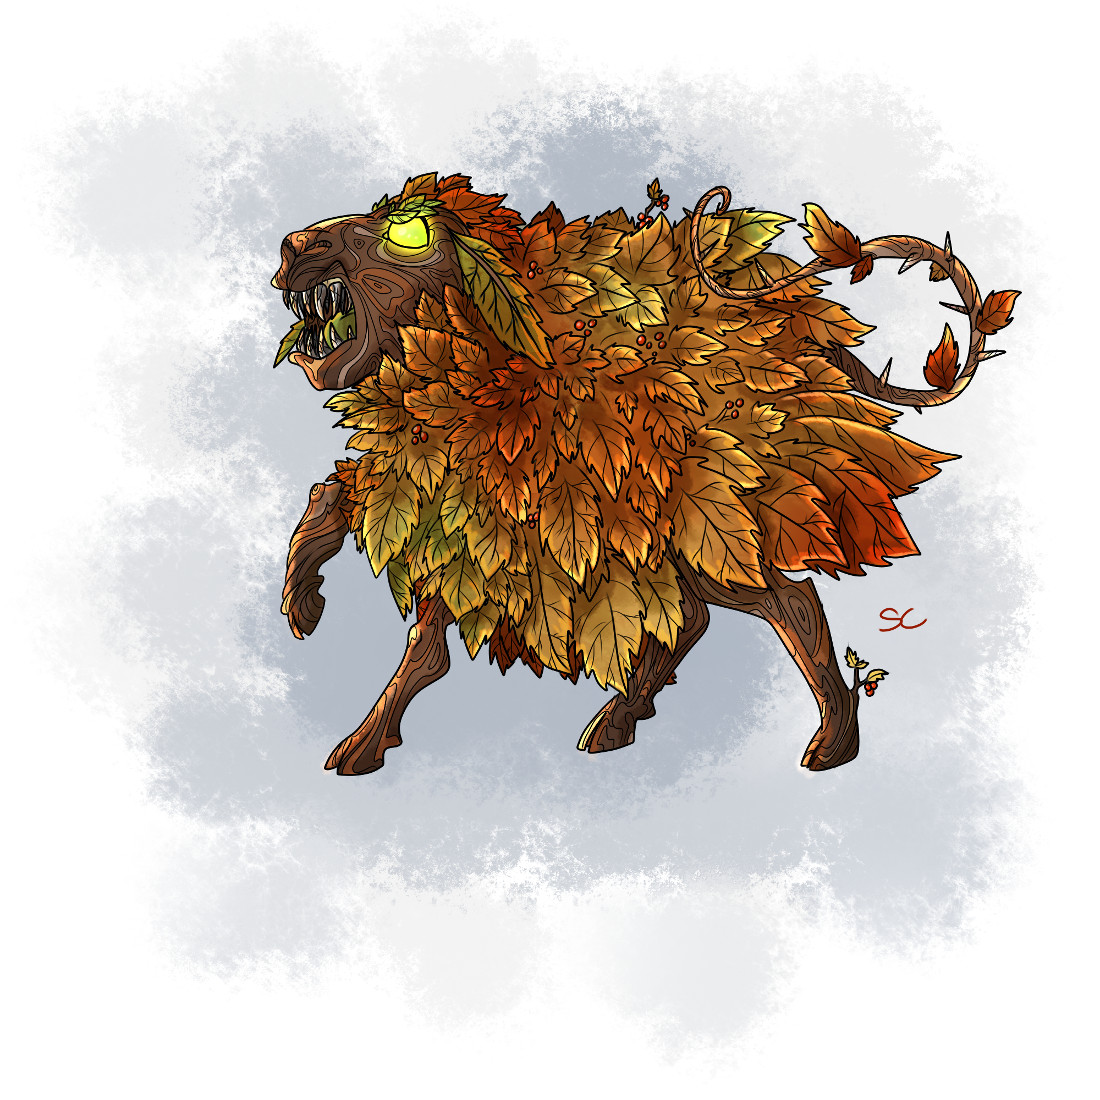
\includegraphics[width=0.5\linewidth]{ART/Enemies/weedling}
	\end{wrapfigure}
	
	Weedlings are lamb-like creatures that are small in stature, barely bigger than a general lap dog. Unlike lap dogs, they're armed with a nasty temper and a herd mentality to take down their prey.
	
	Likely a magical construct similar to the timberwolves, weedlings are wooden lambs with thick bush of leaves for their wool, with an occasional cluster of red berries here and there. Male weedlings tend to have more berries than the females. Much like timberwolves, the weedling's eyes shine in a green color.
	
	Though weedlings are harmless on their own, the herds they gather can and often do prove fatal for a pony, as they rush to knock their targets prone in order to devour them. This is why the weedlings always appear as a swarm, travelling with a large herd of individuals, both for their own protection and to hunt. Weedlings are obligate carnivores despite being a plant.
	
	Due to being a plant, these creatures do stop what they're doing on a sunny day, in order to take in the very few and far between rays of sunshine. This concludes that the weedling can and do photosynthesize, but due to the rarity of it, have developed other means to gather nutrients.
	
	When not actively hunting, the weedlings spend most of their time resting, blending into their forest-like surroundings by curling up, making them resemble nothing more than a regular bush. This is both to hide themselves from predators such as the Moss Shambler, and to ambush any creature foolish enough to wander too close.
	Much like most other plants, weedlings are vulnerable to fire, giving off a bright green sparks when set on fire. 
	
	\clearpage

	\section*{Windigo}
	\addcontentsline{toc}{section}{Windigo}
	\begin{quote}
		\emph{``So, surely you've heard the story of the founding of Equestria? Windigos freezing everything solid blah blah and so on. Though, these winter spirits are real, I've seen a few up north. Though our magic lasers do little more than spook them. Honestly, if you want to get them far away from you, either get friendly towards one another or ask around for a Zebra shaman. I think the shaman's a safer bet.''}
		
		\emph{-	Star Paladin Glitter Dust}
	\end{quote}
	
	\emph{\textbf{Type:} Abomination}
	
	\emph{\textbf{EXP:} 400}
	
	{
		\rowcolors{1}{gray!30}{gray!10}
		\begin{tabu} to 150mm{| X[c,1] | X[c,1] | X[c,1] | X[c,1] | X[c,1] | X[c,1] | X[c,1] | X[c,1] |  X[c,3] | X[c,3]| X[c,3] | X[c,3] | X[c,3] |}
			\hline
			\multicolumn{13}{|c|}{\cellcolor{gray!50} Windigo Statistics}                \\ \hline
			S & P & E & C & I & A & L & \cellcolor{gray!50} & HP & DT & AP & Size & Karma \\
			5 & 5 & 7 & 2 & 6 & 7 & 8 & \cellcolor{gray!50} & 8  & 10 & 13 & 0    & -25   \\ \hline
		\end{tabu}
		
		%\emph{*See Additional Combat Details}
	}
	
	\bigskip
	{
		\rowcolors{1}{gray!30}{gray!10}
		\begin{tabu} to 60mm{| X[c,1] | X[c,1] |}
			\hline
			\multicolumn{2}{|c|}{\cellcolor{gray!50} Skills} \\ \hline
			Unarmed & Sneak                                  \\
			70      & 80                                     \\ \hline
		\end{tabu}
		
	}
	
	\subsubsection*{Additional Combat Details:}
	\begin{verse}
		\textbf{Freezing Touch (6 AP):} Direct contact with Windigo causes the target to get Freezing - Status Effect. This attack also deals 40+(1) Cold damage.
	
		\textbf{Chilling Call (1/min, 8 AP):} Windigos can cause a shriek that will send shivers down the spine of even the most battle-hardened wastelanders. Anyone within Large Burst template from the Windigo who fails a CHA check will gain Medium Distraction for 3 turns.
	
		\textbf{Nefarious Spirit:} Windigos are spirits that manifest themselves in equine form. Due to this, conventional, non-magical weapons have a 50\% chance of not dealing damage to Windigos. Magical weaponry like MEWs, Enchanted weapons and Spirits will deal their damage if hit like normal. 
	
		\textbf{Blizzard:} Windigos, as a winter spirit, generate a bitterly cold blizzard where ever they go. Even the sunniest of days will be clouded with dark skies and never-ending snow. This blizzard can cause a Blinded - status effect, with an END roll to resist. If successfully resisted, the Blizzard has no effect for the duration of the battle.
	
		\textbf{Howering:} As spirit of icy winds, Windigos soar through the skie without wings. Their movement is 6 meters (3 Hexes) for 1 AP.
	
		\textbf{Poison Immunity:} As Windigos can hardly be considered alive, they are naturally immune to poisons.
		
		\textbf{Rad Immunity:} Due to the dark, raw magic that empowers the Windigo, they are very well adapted to irradiated areas, even ground zero. They are immune to the effects of Radiation.
	\end{verse}
	
	\subsubsection*{Creature drops:}
	Windigo Heart (1 u. Gem)
	
	\subsection*{Description:}
	Windigos are nefarious spirits, known to bring with them cold and snow. They tend to seek out ponies that share hatred and fights between each other, as it is their primary source of nutrition - and the more hatred they consume, the colder the surroundings of where Windigos roam turn.
	
	Windigos do not directly engage their prey - they stay close enough to feed upon the hatred, but far enough to not make their presence known. It is only when cornered or spotted will they fight with all they got, and preferably with minimal time taken as to not disturb their ``hunting grounds''.
	
	Spotting a Windigo's presence may require some previous knowledge of the area. Sudden drop in temperature or slight snowfall in areas where there usually isn't may indicate towards the nefarious spirit's existence, especially if there's loud arguments or heavy fights in the area. 
	
	
	\clearpage

	\section*{Wood-Rot Wasp}
	\addcontentsline{toc}{section}{Wood-Rot Wasp}
	\begin{quote}
		\emph{``This large mutated wasp goes after ponies due to being attracted to the scent of dead plant matter, such as weapon stocks, grates and caravans. With their drill-like ovipositor, they implant wooden structures with their eggs, and they also use it to make short work of any pony guarding said wooden structure, after which they feast upon the corpse. These creatures have been known to pierce even metal armor. Truly, a magnificent insect!'' }
		
		\emph{-	Acacia Honey, Entomologist}
	\end{quote}
	
	\emph{\textbf{Type:} Mutated Insect}
	
	\emph{\textbf{EXP:} 150}
	
	{
		\rowcolors{1}{gray!30}{gray!10}
		\begin{tabu} to 150mm{| X[c,1] | X[c,1] | X[c,1] | X[c,1] | X[c,1] | X[c,1] | X[c,1] | X[c,1] |  X[c,3] | X[c,3]| X[c,3] | X[c,3] | X[c,3] |}
			\hline
			\multicolumn{13}{|c|}{\cellcolor{gray!50} Wood-Rot Wasp Statistics}           \\ \hline
			S & P & E & C & I & A & L & \cellcolor{gray!50} & HP & DT & AP & Size & Karma \\
			5 & 8 & 3 & 2 & 1 & 8 & 4 & \cellcolor{gray!50} & 10 & 5  & 14 & -1   & 0     \\ \hline
		\end{tabu}
		
		%\emph{*See Additional Combat Details}
	}
	
	\bigskip
	{
		\rowcolors{1}{gray!30}{gray!10}
		\begin{tabu} to 60mm{| X[c,1] | X[c,1] |}
			\hline
			\multicolumn{2}{|c|}{\cellcolor{gray!50} Skills} \\ \hline
			Unarmed & Sneak                                  \\
			40      & 40                                     \\ \hline
		\end{tabu}
		
	}

	\subsubsection*{Additional Combat Details:}
	\begin{verse}
		\textbf{Stinger (4 AP):} The Wood-Rot Wasp doesn't have a stinger per say, but its ovipositor has ``teeth'' that make it function like a drill, which it can use to defend itself. The attack deals 30+(2) damage, and ignores 20 DT.
	
		\textbf{Flying:} Wood-Rot Wasps did not retain their speed, only flying at a pace of 2 meters (1 Hex) for 1 AP.
	
		\textbf{Quick Flier:} Wood-Rot Wasps are fast, and due to this they get a +2 to their Initiative rolls.
	
		\textbf{Insect Brain:} Crippling the Wood Rot Wasp's antennae causes it to gain Mind Controlled and Enraged -status effects and make them attack the nearest creature, be it friend or foe.
	
		\textbf{Poison Resistant:} Wood-Rot Wasp is relatively resistant to poisons, with their poison resistance being 40.
	
		\textbf{Rad Resistant:} Wood-Rot Wasp is an insect mutated by balefire fallout, gaining a decent resistance to the radiation. Wood-Rot Wasp's Rad Resistance is 50.
	\end{verse}
	
	\subsubsection*{Creature drops:}
	\begin{compactitem}
		\item Wood-Rot Wasp eggs (1d4, Survival doubles u.)
		\item Wood-Rot Wasp Stinger (Stinger, 1 u.)
	\end{compactitem}
	
	\subsection*{Description:}
	Wood-Rot Wasps are -for an insect- a large parasitoid wasp species mutated by balefire. Their most notable feature is their long stinger-like ovipositor, that they use to both fend for themselves or to lay their eggs in rotting wood, hence their name.
	
	Though they are not very aggressive, often leaving wandering ponies alone unless they feel threatened, they will attack any creature that stands between any sufficient rotting wood, be it structures, wagons or dead trees when they attempt to lay their eggs. Wood-rot wasps seem to locate the wood by scent. They can also use plant-like mutants, such as the Moss Shambler or Spore Carrier for their egg-laying.
	
	Due to the fact that females are the only ones with an ovipositor, only the females are harmful to ponies, while male wood-rot wasps are both smaller and feed entirely on nectar and other insects, such as Twittermite. The female wood-rot wasps lay 7-10 eggs inside the wood, which eventually, in a span of several months, spring forth fully developed, as their life-cycle is very fast. The adult wood-rot wasps live for a few weeks at maximum.
	
	\clearpage

	\section*{Yao Guai}
	\addcontentsline{toc}{section}{Yao Guai}
	\begin{quote}
		\emph{``Yao Guai is essentially a mutated bear that has lost its fur and gained vicious temper in return. They're aggressive, with mass and power to back it up. And unlike the bears of old, these ones do not run away when they smell you, they run at you, ready to really buck your day. As far as I have heard, honey might still be delicious to them. Maybe. I would at least advice one not to carry a jar with them when taking a leisurely stroll through the woods. Or a picnic basket, for that matter.''}
	
		\emph{-	Verdant Brink, Hunter}
	\end{quote}
	
	\emph{\textbf{Type:} Mutated Animal}
	
	\emph{\textbf{EXP:} 500}
	
	{
		\rowcolors{1}{gray!30}{gray!10}
		\begin{tabu} to 150mm{| X[c,1] | X[c,1] | X[c,1] | X[c,1] | X[c,1] | X[c,1] | X[c,1] | X[c,1] |  X[c,3] | X[c,3]| X[c,3] | X[c,3] | X[c,3] |}
			\hline
			\multicolumn{13}{|c|}{\cellcolor{gray!50} Yao Guai Statistics}           \\ \hline
			S & P & E & C & I & A & L & \cellcolor{gray!50} & HP & DT & AP & Size & Karma \\
			8 & 6 & 7 & 4 & 3 & 4 & 4 & \cellcolor{gray!50} & 18 & 30 & 12 & 1    & 0     \\ \hline
		\end{tabu}
		
		%\emph{*See Additional Combat Details}
	}
	
	\bigskip
	{
		\rowcolors{1}{gray!30}{gray!10}
		\begin{tabu} to 60mm{| X[c,1] | X[c,1] |}
			\hline
			\multicolumn{2}{|c|}{\cellcolor{gray!50} Skills} \\ \hline
			Unarmed & Sneak                                  \\
			70      & 60                                     \\ \hline
		\end{tabu}
		
	}
	
	\subsubsection*{Additional Combat Details:}
	\begin{verse}
		\textbf{Bite (8 AP):} Yao Guai sometimes use their powerful jaws to cripple and pacify their foes, dealing 40+(4) damage and have a base crippling chance of 20\% with this attack.
	
		\textbf{Claws (6 AP):} The Yao Guai's claws can rip apart the weakest armors in seconds. The attack deals 30+(3) damage, and ignores 10 DT.
	
		\textbf{Long reach:} Yao Guai have considerably long forelegs, giving their Melee and Unarmed attacks additional 2 meters (1 Hex) reach.
	
		\textbf{Tight Grasp:} Yao Guai's strong forelegs make them excellent at grappling their foes, thus they gain +10 to all opposed rolls made to Grapple.
	
		\textbf{Woodlands Stride:} Yao Guai are capable of surprisingly agile movements for their size and weight, thus ignoring the +1 AP cost of Difficult Terrain.
	
		\textbf{Poison Resistant:} Despite being mutated creatures, Yao Guai are quite weak against toxins. Yao Guai's Poison Resistance is 20.
	
		\textbf{Rad Resistant:} As Balefire-mutated creatures, Yao Guai are reasonably equipped against radiation. Yao Guai's Rad Resistance is 50.
	\end{verse}
	
	\subsubsection*{Creature drops:}
	\begin{compactitem}
		\item Yao Guai Meat (1d4 pieces, Survival doubles u.)
		\item Hide (1d4 pieces, Survival doubles u.)
		\item Paw (4 u.)
		\item Yao Guai Crystals (1d4, Survival doubles u. Gem)
	\end{compactitem}
	
	\subsection*{Ghoulified Yao Guai}
	\addcontentsline{toc}{subsection}{Ghoulified Yao Guai}
	\begin{quote}
		\emph{``It is safe to say the rookies do fear the bear despite their mighty armor. And while many of them may live to tell against such encounters, without a single scratch, such fear is negligible. However.. there is a true nightmare as well. The elder Yao Guai as some call them, are the pinnacle beasts of terror. Further gone through mutation by Radiation, their size is much larger, their claws greater, and you bet their stench does bypass the filter.''}
		
		\emph{-	Star Paladin Glitter Dust}
	\end{quote}
	
	\emph{\textbf{Type:} Abomination}
	
	\emph{\textbf{EXP:} 650}
	
	{
		\rowcolors{1}{gray!30}{gray!10}
		\begin{tabu} to 150mm{| X[c,1] | X[c,1] | X[c,1] | X[c,1] | X[c,1] | X[c,1] | X[c,1] | X[c,1] |  X[c,3] | X[c,3]| X[c,3] | X[c,3] | X[c,3] |}
			\hline
			\multicolumn{13}{|c|}{\cellcolor{gray!50} Ghoulified Yao Guai Statistics}      \\ \hline
			S  & P & E & C & I & A & L & \cellcolor{gray!50} & HP & DT & AP & Size & Karma \\
			10 & 6 & 8 & 3 & 2 & 4 & 4 & \cellcolor{gray!50} & 18 & 30 & 12 & 2    & 0     \\ \hline
		\end{tabu}
		
		%\emph{*See Additional Combat Details}
	}
	
	\bigskip
	{
		\rowcolors{1}{gray!30}{gray!10}
		\begin{tabu} to 60mm{| X[c,1] | X[c,1] |}
			\hline
			\multicolumn{2}{|c|}{\cellcolor{gray!50} Skills} \\ \hline
			Unarmed & Sneak                                  \\
			75      & 60                                     \\ \hline
		\end{tabu}
		
	}
	
	\subsubsection*{Additional Combat Details:}
	\begin{verse}
		\textbf{Bite (8 AP)}: Yao Guai sometimes use their powerful jaws to cripple and pacify their foes, dealing 50+(4) damage and have a base crippling chance of 20\% with this attack.
	
		\textbf{Claws (6 AP):} The Yao Guai's claws can rip apart the weakest armors in seconds. The attack deals 30+(4) damage, and ignores 20 DT.
	
		\textbf{Irradiated attacks:} Ghoulified Yao Guai's attacks carry Radiation. Every attack has a 1 x 60\% chance of giving a Rad token. 
	
		\textbf{Long reach:} Ghoulified Yao Guai have considerably long forelegs, giving their Melee and Unarmed attacks additional 4 meters (2 Hex) reach.
	
		\textbf{Tight Grasp:} Ghoulified Yao Guai's strong forelegs make them excellent at grappling their foes, thus they gain +10 to all opposed rolls made to Grapple.
	
		\textbf{Woodlands Stride:} Ghoulified Yao Guai are capable of surprisingly agile movements for their size and weight, thus ignoring the +1 AP cost of Difficult Terrain.
	
		\textbf{Poison Resistant:} Despite further mutations, Ghoulfied Yao Guai are quite weak against toxins. Yao Guai's Poison Resistance is 25.
	
		\textbf{Rad Immunity:} Through further extended exposure to Radiation, Ghoulified Yao Guai have developed full immunity to Radiation.
	\end{verse}
	
	\subsubsection*{Creature drops:}
	\begin{compactitem}
		\item Ghoulified Yao Guai Meat (Abomination Flesh Piece, 1d4 pieces, Survival doubles u.)
		\item Ghoulified Yao Guai Hide (Irradiated Material, 1d4 pieces, Survival doubles u.)
		\item Paw (4 u.)
		\item Yao Guai Crystals (1d4, Survival doubles u. Gem)
	\end{compactitem}
	
	\subsection*{Description:}
	The Yao Guai are bears that have either lost most of their fur, or have crystalline growth and studs across their bodies. In comparison to a normal bear, they also stand taller and mightier.
	
	The origins of the term ``Yao Guai'' to name the horribly mutated bears with short temper and a lot of aggression have been lost to the time, a few arguing it may have its origins in Zebra language. Whatever the case may be, it is clear the Yao Guai do not care what you call them, only that their domain is left alone. And most often said domain is ``50 meter radius from where one is currently standing''. 
	
	The further mutation of Yao Guai, through massive Radiation exposure has reduced them in much more feral, solely on instinct driven state. However, such development has increased their size and strength considerably, while also making them impervious to Radiation, even radiating it themselves.
	
	Otherwise in behaviour, the Yao Guai do not differ from unmutated bears. They are most often solitary creatures, only meeting others of their kind for breeding purposes, and the mother looks after the newly-born Yao Guai cubs until they're large enough to defend themselves. If one does meet a Yao Guai cub on its own, the mother is close by - and viciously defends its offspring.
	
	\clearpage

	\section*{Zebra}
	\addcontentsline{toc}{section}{Zebra}
	\begin{quote}
		\emph{``What is there to be said about Zebra, the distant and distinct kin of ours? Their strange customs and beliefs continue to confound me to this day, not to mention the way most of them speak, in rhyme no less! But I wager, if they're not on the warpath, you could have a chat with them. And if they are... run.''}
		
		\emph{-	Merchant Silver Bit}
	\end{quote}
	
	\emph{\textbf{Type:} Sentient}
	
	\emph{\textbf{EXP:} 200}
	
	{
		\rowcolors{1}{gray!30}{gray!10}
		\begin{tabu} to 150mm{| X[c,1] | X[c,1] | X[c,1] | X[c,1] | X[c,1] | X[c,1] | X[c,1] | X[c,1] |  X[c,3] | X[c,3]| X[c,3] | X[c,3] | X[c,3] |}
			\hline
			\multicolumn{13}{|c|}{\cellcolor{gray!50} Zebra Statistics}                         \\ \hline
			S & P & E & C & I & A & L & \cellcolor{gray!50} & HP & DT     & AP & Size & Karma   \\
			5 & 5 & 4 & 7 & 7 & 7 & 6 & \cellcolor{gray!50} & 14 & Varies & 13 & 0    & Varies* \\ \hline
		\end{tabu}
		
		\emph{*Karma varies based on the individual}
	}
	
	\bigskip
	{
		\rowcolors{1}{gray!30}{gray!10}
		\begin{tabu} to 150mm{| X[c,1] | X[c,1] | X[c,1] | X[c,1] | X[c,1] | X[c,1] |}
			\hline
			\multicolumn{6}{|c|}{\cellcolor{gray!50} Skills}        \\ \hline
			Firearms & Melee & Unarmed & Sneak & Barter & Diplomacy \\
			60       & 50    & 60      & 70    & 70     & 40        \\ \hline
		\end{tabu}
		
	}
	
	\subsubsection*{Additional Combat Details:}
	\begin{verse}
		\textbf{Wasteland Weaponry:} Zebras can carry just about any weapon and armor imaginable, though often preferring their own heritage weapons. 
	
		\textbf{Shamanism:} Some zebras can use Spirits in battle, as per Tribal Shaman trait.
		
		\textbf{Alchemical Interests:} Zebras know how to brew potions and poisons, and do not shy from using them.
		
		\textbf{Abomination Hunter:} Due to their high-caliber weaponry and armor, most zebras are well-equipped to fight even the most horrid things the Wasteland has to offer. They gain a +10 to Combat skills when targeting Abominations, excluding sane Ghouls.
	
		\textbf{Zebra Language:} Zebra speak their own native language, often allowing them to strategize on the battlefield without their enemy catching on. Characters that understand Zebra language can interpret them, however.
	
		\textbf{Poison Resistant:} Zebra boast higher natural poison resistance to ponies, and often use armor to further boost their defenses. Zebra's natural poison resistance is 20.
	
		\textbf{Rad Resistant:} Zebra are just as weak to the magical radiation as their pony counterparts, giving them 5 Rad Resistance. However, they may equip armor to shield themselves from this danger.
	\end{verse}
	
	\subsubsection*{Creature drops:}
	\begin{compactitem}
		\item Main Weapon (1 u.)
		\item Additional Weapon (1-2 u.)
		\item Armor or Clothing (1 u.)
		\item Healing Item or Alchemical brew (1, LCK doubles)
		\item Alchemical recipe (LCK-2 to obtain)
	\end{compactitem}
	
	\subsection*{Description:}
	Zebras, the striped equine cousins of ponies, weren't exterminated by the balefire exchange between their now-fallen nation and Equestria during the Great War, just like Equestrian ponies weren't. Zebras have endured and improvised the fall of civilization while not letting their past rituals and cultural aspects get lost in time.
	
	Zebras, like ponies, are social individuals - they have their own goals and desires, though survival brings them closer to other, like-minded fellows. Thus zebras aren't inherently evil or good, it depends on the particular individual.
	
	Some zebras may have wandered to the Equestrian Wasteland from their own lands, while some are the descendants of zebras that lived in pre-War Equestria. While a few reside with ponies in same settlements, the past deeds and mistrust runs deep in some ponies, and zebras are more often than not shunned by pony communities. It is thus not unheard of zebras forming their own communities in the wilderness or ruins, away from those who may seek harm to them.
	
	\clearpage

	\chapter*{Critters by Category}
	\addcontentsline{toc}{chapter}{Critters by Category}
	{
		\rowcolors{1}{gray!30}{gray!10}
		\begin{tabu} to 160mm{| X[l,1] | X[l,4] |}
			\hline
			\cellcolor{gray!50} Type & \cellcolor{gray!50} Critters                                                                                                                                           \\ \hline
			Abomination              & Alicorns, Necrosprite, Brahmin, Chimera, Feral Mongrel, Ghouls, Ghost, Hellhound, Hospital Horror, Myling, Radstag, Shade, Spore Carrier, Windigo, Ghoulified Yao Guai \\
			Animal, Mutated          & Balefire Phoenix, Bloodwing, Feral Dog, Geckos, Molerat, Radbit, Radhog, Radrel, Salamander,  Radigators, Snakes, Yao Guai                                             \\
			Animal, Non-Mutated      & Cockatrice, Hydra, Jackalopes, Manticore, Quarray Eel, Star-Spawn, Timberwolf                                                                                          \\
			Insect, Mutated          & Bloatsprite, Necrosprite, Fire Ants, Giant Ants, Rad-Butterfly, Radroach, Radscorpion, Spiders, Tankbug, Wood-Rot Wasp                                                 \\
			Insect, Non-Mutated      & Bugbear, Flash Bee, Twittermite                                                                                                                                                            \\
			Machine                  & Equitron, Mister Hoofies, Robobrain, Sprite Bot, Turret,   Spider-Bot, Ultra-Sentinel                                                                                  \\
			Plant, Mutated           & Firebush, Floater, Moss Shamblers, Spore Carrier,  Spore Plant, Triggerbloom, Weedling                                                                                 \\
			Sentient                 & Alicorns, Changeling, Dragon, Enclave, Hellhound, Mercenary, Raider, Slaver, Steel Ranger, Thug, Zebra                                                                 \\ \hline
		\end{tabu}
		
	}

\end{document}